% August 2017 (TOC contents linked in blue in pdf file)
%This template was prepared by Dorothea F. Brosius of the
%Institute for Electronics and Applied Physics, University of Maryland, College Park, MD
%The template was last updated in August 2017
%Thesis Main Page used with thesis.sty based on the
%University of Maryland Electronic Thesis and Dissertation (ETD) Style Guide (2016)

%The YourInformation file was created by Freja Nordsiek, 2014.
%Code for linking the TOC titles to the text in the pdf file was created by Freja Nordsiek, 2014.

% Select the version that fits how you are making this LaTeX document (its driver).
% The first two are the most likely ones to be needed.

 \newcommand{\mydriver}{pdflatex} %Making a PDF directly using pdflatex.
%\newcommand{\mydriver}{dvipdfmx} %Making a DVI and converting that to PDF using dvipdfmx.
%\newcommand{\mydriver}{dvipdfm} %Making a DVI and converting that to PDF using dvipdfm.
%\newcommand{\mydriver}{dvips} %Making a DVI and converting that to PS using dvips (may later be converted to PDF).
%\newcommand{\mydriver}{dvipsone} %Making a DVI and converting that to PS using dvipsone (may later be converted to PDF).
%\newcommand{\mydriver}{ps2pdf} %Same as the one for dvips except it is compatible with Ghostscript's PDF writer.
\newcommand{\swave}[0]{$\it{s}$-wave}
\newcommand{\pwave}[0]{$\it{p}$-wave}
\newcommand{\K}{$^{40}\rm{K}$}
\newcommand{\Rb}{$^{87}\rm{Rb}$}
\newcommand{\us}{$\rm{\mu s}$}
\newcommand{\mT}{$\rm{mT}$}
\newcommand{\ez}{$\bf{\mathit{e}_z}$}
\newcommand{\ex}{$\bf{\mathit{e}_x}$}
\newcommand{\um}{$\rm{\mu m}$}
\renewcommand{\thefootnote}{\arabic{footnote}}

\documentclass[12pt,\mydriver]{umdthesis-2}  %12pt is larger than 11pt

\usepackage{titlesec}
   \titleformat{\chapter}
      {\normalfont\large}{Chapter \thechapter:}{1em}{}
\usepackage{amsmath}
\usepackage{graphicx}
\usepackage{cite}
\usepackage{lscape}
\usepackage{indentfirst}
\usepackage{latexsym}
\usepackage{multirow}
\usepackage{epstopdf}
\usepackage{tabls}
\usepackage{wrapfig}
\usepackage{slashbox}
\usepackage{longtable}
\usepackage{supertabular}
%\usepackage{subeqn}
\usepackage{subfigure}
\usepackage{braket}
\usepackage{algorithmic}
\usepackage{algorithm}

%hyperref
\usepackage[colorlinks=true,urlcolor=black,linkcolor=blue,citecolor=blue]{hyperref}

\newcommand{\tbsp}{\rule{0pt}{18pt}} %used to get a vertical distance after \hline
\renewcommand{\baselinestretch}{2}
\setlength{\textwidth}{5.9in}
\setlength{\textheight}{9in}
\setlength{\topmargin}{-.50in}
%\setlength{\topmargin}{0in}    %use this setting if the printer makes the the top margin 1/2 inch instead of 1 inch
\setlength{\oddsidemargin}{.55in}
\setlength{\parindent}{.4in}
\pagestyle{empty}

\begin{document}
\pagestyle{empty}
%Abstract Page

\hbox{\ }

\renewcommand{\baselinestretch}{1}
\small \normalsize

\begin{center}
\large{{ABSTRACT}}

\vspace{3em}

\end{center}
\hspace{-.15in}
\begin{tabular}{ll}
Title of dissertation:    & {\large  Direct measurement of a Feshbach resonance with imaging of s-wave scattering}\\
&                     {\large  } \\
&                     {\large and measuring topology of BECs in a synthetic dimensions lattice} \\
\ \\
&                          {\large  Dina Genkina} \\
&                           {\large Doctor of Philosophy, 2018} \\
\ \\
Dissertation directed by: & {\large  Professor Ian Spielman} \\
&               {\large  Department of Physics } \\
\end{tabular}

\vspace{3em}

\renewcommand{\baselinestretch}{2}
\large \normalsize

 %(must be first, required, non-numbered)
%Titlepage

\thispagestyle{empty}
\hbox{\ }
\vspace{1in}
\renewcommand{\baselinestretch}{1}
\small\normalsize
\begin{center}

\large{{NONLINEAR PULSE PROPAGATION THROUGH \\
AN OPTICAL FIBER : THEORY AND EXPERIMENT}}\\
\ \\
\ \\
\large{by} \\
\ \\
\large{Bhaskar Khubchandani}%Your full name as it appears in University records.
\ \\
\ \\
\ \\
\ \\
\normalsize
Dissertation submitted to the Faculty of the Graduate School of the \\
University of Maryland, College Park in partial fulfillment \\
of the requirements for the degree of \\
Doctor of Philosophy \\
2004
\end{center}

\vspace{7.5em}

\noindent Advisory Committee: \\
Professor Rajarshi Roy, Chair/Advisor \\
Dr. Parvez N. Guzdar, Co-Advisor \\
Professor Robert W. Gammon \\
Professor Thomas Antonsen \\
Professor Edward Ott
 %(must follow Abstract, required, non-numbered)
%Copyright

\thispagestyle{empty}
\hbox{\ }

\vfill
\renewcommand{\baselinestretch}{1}
\small\normalsize

\vspace{-.65in}

\begin{center}
\large{\copyright \hbox{ }Copyright by\\
Dina Genkina  %Type your name as it appears in University records
\\
2019}
\end{center}

\vfill

\newpage

\hbox{\ }
\newpage
 %(highly recommended, non-numbered)

%Pages from this point start at lower-case Roman number ii)
%\pagestyle{plain} \pagenumbering{roman} \setcounter{page}{2}
%\addcontentsline{toc}{chapter}{Preface}
%%Preface
\pagestyle{plain}\pagenumbering{roman} \setcounter{page}{2}
\renewcommand{\baselinestretch}{2}
\small\normalsize
\hbox{\ }

\vspace{-.65in}

\begin{center}
\large{Preface}
\end{center}


If needed.
  %(if present, start at lower-case Roman number ii)
%\addcontentsline{toc}{chapter}{Foreword}
%%Foreword

\renewcommand{\baselinestretch}{2}
\small\normalsize
\hbox{\ }
 
\vspace{-.65in}

\begin{center}
\large{Foreword} 
\end{center} 

If needed.
 %(if present, lower-case Roman)
%\addcontentsline{toc}{chapter}{Dedication}
%%Dedication

\renewcommand{\baselinestretch}{2}
\small\normalsize
\hbox{\ }
 
\vspace{-.65in}

\begin{center}
\large{Dedication}
\end{center} 

If needed.
 %(if present, lower-case Roman)
%\addcontentsline{toc}{chapter}{Acknowledgements}
%%Acknowledgments

\renewcommand{\baselinestretch}{2}
\small\normalsize
\hbox{\ }
 
\vspace{-.65in}

\begin{center}
\large{Acknowledgments} 
\end{center} 

\vspace{1ex}

I owe my gratitude to all the people who have made this thesis possible and because of whom my graduate experience has been one that I will cherish forever.

First and foremost I'd like to thank my advisor, Professor Rajarshi Roy for giving me an invaluable opportunity to work on challenging and extremely interesting projects over the past four years. He has always made himself available for help and advice and there has never been an occasion when I've knocked on his door and he hasn't given me time. It has been a pleasure to work with and learn from such an extraordinary individual.

I would also like to thank my co-advisor, Dr. Parvez Guzdar. Without his extraordinary theoretical ideas and computational expertise, this thesis would have been a distant dream. Thanks are due to Professor Robert Gammon, Professor Edward Ott and Professor Thomas Antonsen for agreeing to serve on my thesis committee and for sparing their invaluable time reviewing the manuscript.

My colleagues at the nonlinear optics laboratory have enriched my graduate life in many ways and deserve a special mention. David DeShazer helped me start-off by rewriting the basic simulation code in a user-friendly format. Christian Silva provided help by setting up the GRENOUILLE apparatus and performing some of the simulations. My interaction with  Rohit Tripathi, Ryan McAllister, Vasily Dronov, Min-Young Kim, Elizabeth Rogers, William Ray, Jordi Garcia Ojalvo, Riccardo Meucci, Atsushi Uchida, and Fabian Rogister has been very fruitful. I'd also like to thank Wing-Shun Lam and Benjamin Zeff for providing the LaTex style files for writing this thesis.

I would also like to acknowledge help and support from some of the staff members. Donald Martin's technical help is highly appreciated, as is the computer hardware support from Edward Condon, LaTex and software help from Dorothea Brosius and purchasing help from Nancy Boone.

I owe my deepest thanks to my family - my mother and father who have always stood by me and guided me through my career, and have pulled me through against impossible odds at times. Words cannot express the gratitude I owe them. I would also like to thank Dr. Mohan Advani, Dr. Vasudeo Paralikar and Dr. Vinod Chaugule who are like family members to me.

My housemates at my place of residence have been a crucial factor in my finishing smoothly. I'd like to express my gratitude to Sivasankar Pandeti, Jayakumar Patil, Amit Trehan and Punyaslok Purakayastha for their friendship and support.

I would like to acknowledge financial support from the Office of Naval Research (ONR), Physics, for all the projects discussed herein.

It is impossible to remember all, and I apologize to those I've inadvertently left out.

Lastly, thank you all and thank God!
 %(if present, lower-case Roman)

%\renewcommand{\baselinestretch}{1}
%\small\normalsize
%\tableofcontents %(required, lower-case Roman)
%\newpage
%\listoftables %(if present, lower-case Roman)
%\newpage
%\listoffigures %(if present, lower-case Roman)
%\newpage
%% LIST OF ABBREVIATIONS
%\addcontentsline{toc}{chapter}{List of Abbreviations}
%%List of Abbreviations


\renewcommand{\baselinestretch}{1}
\small\normalsize
\hbox{\ }

\vspace{-4em}

\begin{center}
\large{List of Abbreviations}
\end{center} 

\vspace{3pt}

\begin{supertabular}{ll}
AAA & Antiaircraft artillery \\
ABCCC & Airborne Battlefield Command and Control Center \\
AEHF & Advanced Extremely High Frequency \\
AGM & Air-to-ground guided missile \\
AIT & Assembly, Integration, and Testing \\
AOR & Area of Responsibility \\
APAM & Anti-personnel, anti-material \\
ASOC & Air Support Operations Center \\
ATACM & Army Tactical Missile System \\
ATO & Air Tasking Order \\
AWACS & Airborne Warning and Control System \\
\\
BAT & Brilliant Ani-Armor Submunition \\
BDA & Bomb-damage assessment  \\
BFT & Blue Force Tracking \\
BLOS & Beyond Line-of-Sight \\
BMD & Ballistic Missile Defense \\
\\
C$^{3}$ & Command, Control, and Communications \\
CAFMS & Computer-aided Force Management System \\
CALCM & Conventional Air-Launched Cruise Missile \\
CBU & Cluster Bomb Unit \\
CCAFS & Cape Canaveral Air Force Station \\
CENTAF & CENTCOM's Air Force component \\
CENTCOM & U.S. Central Command \\
CINC & Commander-in-Chief \\
CONUS & Continental United States \\
\\
DAGR & Defense Advanced GPS Reciever \\
DMA & Defense Mapping Agency \\
DOD & Department of Defense \\
DOP & Dilution of Precision \\
DOT & Department of Transportation \\
DSMAC & Digital Scene Mapping Area Correlator \\
\\
EFOG-M & Enhanced Fiber Optic Guided Missile \\
\\
FAA & Federal Aviation Administration \\
FLIR & Forward-looking infrared \\
\\
GAM & Global Positioning System Aided Munition \\
GPS & Global Positioning System \\
GWAPS & Gulf War Air Power Survey \\
\\
HARM & High-Speed Antiradiation Missile \\
HEO & Highly Elliptical Orbit \\
\\
IADS & Integrated Air Defense System \\
ICBM & Inter-Continental Ballistic Missile \\
INS & Inertial navigation system \\
IIR & Imaging infrared \\
IR & Infrared \\
ISR & Intelligence, Surveillance, and Reconnaissance \\
\\
JDAM & Joint Direct Attack Munition \\
JFC & Joint Force Commander \\
JSOW & Joint Standoff Weapon \\
\\
LANTIRN & Low-Altitude Navigation and Targeting Infrared for Night System \\
LEO & Low Earth Orbit \\
LGB & Laser-guided bomb \\
\\
MAJIC & Microsatellte Area-Wide Joint Information Communication \\
MARCENT & CENTCOM's Marine component \\
MARS & Mid-Atlantic Regional Spaceport \\
MLRS & Multiple Launch Rocket System \\
MUOS & Mobile User Objective System \\
\\
NASA & National Aeronautics and Space Administration \\
NAVCENT & CENTCOM's Navy component \\
NPOESS & National Polar-Orbiting Operational Environmental Satellite System \\
\\
ORS & Opertionally Responsive Space \\
ORSO & Operationally Responsive Space Office \\
\\
PDOP & Position Dilution of Precision \\
PGM & Precision-guided munition \\
P$^{3}I$ & Preplanned Product Improvement \\
PnP & Plug and Play \\
PnPSat & Plug and Play Satellite \\
PPS & Precise Positioning Service \\
\\
RCS & Radar cross section \\
\\
SA & Situational Awareness \\
SADARM & Sense and Destroy Armor Munition \\
SAM & Surface-to-air missile \\
SAR & Synthetic aperture radar \\
SBIRS & Space Based Infrared System \\
SEAD & Suppression of enemy air defenses \\
SFW & Sensor Fuzed Weapon \\
SIGINT & Signal Intelligence \\
SLAM & Standoff Land Attack Missile \\
SLAM-ER & SLAM-Expanded Response \\
SpaceX & Space Exploration Technologies Corporation \\
SPS & Standard Positioning Service \\
\\
TACC & Tactical Air Control Center \\
TACS & Tactical Air Control System \\
TACP & Tactical Air Control Party \\
TASM & Tomahawk Anti-Ship Missile \\
TBIP & Tomahawk Baseline Improvement Program \\
TERCOM & Terrain Contour Mapping \\
TFR & Terrain-following radar \\
TLAM & Tomahawk Land Attack Missile \\
\\
USAF & U.S. Air Force \\
\\
VAFB & Vandenberg Air Force Base \\
\\
WGS & Wideband Global SATCOM \\
%$\alpha$ & alpha \\
%$\beta$  & beta \\
%&  \\ 
%IREAP & Institute for Research in Electronics and Applied Physics \\
%NSA & National Security Agency
\end{supertabular}


%\newpage
%\setlength{\parskip}{0em}
%\renewcommand{\baselinestretch}{2}
%\small\normalsize

%Pages from this point start at Arabic numeral 1
%\setcounter{page}{1}
%\pagenumbering{arabic}
%%Chapter 1

\renewcommand{\thechapter}{1}

\chapter{Introduction}

\section{Source of Nonlinearity in an Optical Fiber}

The response of any dielectric to light becomes nonlinear
for intense electromagnetic fields.  Standard optical fibers are made of
fused silica which is a dielectric. The total polarization $\bf{P}$
is nonlinear in the electric field $\bf{E}$ and is given by [1-5] -
%\cite{Agrawal1,Bloembergen,Shen,Butcher,Boyd} -
%1.1
\begin{equation}
{\bf P} = \epsilon_{0} \left( \chi^{(1)} : {\bf E} + \chi^{(2)}
: {\bf EE} + \chi^{(3)} : {\bf EEE} + \ldots \right),
\end{equation}
where $\epsilon_0$ is the permittivity of free-space, and
$\chi^{(j)}$
is the ${\it j}$-th order susceptibility of the dielectric. The linear
susceptibility $\chi^{(1)}$ represents the dominant contribution to
$\bf{P}$ and its effects are included through the refractive index
n($\omega$) and the attenuation coefficient $\alpha(\omega)$. $\chi^{(2)}$
is responsible for nonlinear effects such as sum-frequency generation and
second harmonic generation \cite{Agrawal1, Shen}. Fused silica does not
manifest these effects as it is centro-symmetric \cite{Newell}. Hence, the dominant nonlinear
contribution to ${\bf P}$ is due to $\chi^{(3)}$ which results in effects
such as third harmonic generation, four-wave-mixing,  self- and
cross-phase modulation. The cubic nonlinearity results in an intensity
dependent refractive index

\begin{verbatim}
122 23333
1114    14444
\end{verbatim}

%1.2
\begin{equation}
\tilde{n}(\omega,|E|^2) = n(\omega)+n_2|E|^2 ,
\end{equation}
where n($\omega$) is the linear part given by the Sellmier
equation which
takes into account the resonance frequencies ($\omega_j$) of fused
silica \cite{Agrawal1,Marcuse},
%1.3
\begin{equation}
n^2(\omega) = 1 + \sum_{j=1}^m {B_j\omega^2_j \over \omega^2_j - \omega^2}
\end{equation}
and n$_2$ is given by
%1.4
\begin{equation}
n_2 = {3 \over 8n}Re(\chi_{xxxx}^3)
\end{equation}
for an optical wave assumed to be linearly polarized along one of the
axes of a polarization maintaining fiber. The tensorial nature of $\chi^{(3)}$ needs to be
considered for the case in which the light is not polarized along one of
the fiber axes.\footnote{This is my footnote.  I started playing the piano when I was eight years old.  This is my footnote.  I started playing the piano when I was eight years old.  This is my footnote.  I started playing the piano when I was eight years old.  This is my footnote.  I started playing the piano when I was eight years old.}

The following is an equation array to ensure the long equation does not go outside the margins.
\begin{eqnarray}
W & = & \int d^3{\bf r} \left[ \sum_s \left( \int d^3{\bf v} {T_{0s} \langle h^2_s \rangle {\bf r} \over 2F_{0s}} - {q^2_s\varphi^2 n_{0s} \over T_{0s}} \right) + {|\delta {\bf B}|^2 \over 8 \pi} \right] \nonumber \\
& = & \int d^3{\bf r} \left( \sum_s \int d^3{\bf v} {T_{0s}\delta f^2_s \over 2F_{0s}} + {|\delta {\bf B}|^2 \over 8\pi} \right) .
\end{eqnarray}

The experimentally measured value of $n_{2}$ for fused silica ranges from $2.2 - 3.4 \times
10^{-20}$\,m$^2$/W, which is small compared to most other nonlinear media by
at least 2 orders of magnitude \cite{Agrawal1}. Despite this, nonlinear effects are
easily observed for silica fibers for relatively low input power levels due
to the fact that the effective fiber core areas are small and the fiber losses are low.
Single mode fibers (those which propagate a single transverse mode of light for a given
wavelength) have effective fiber core diameters of the order of 5$\mu$m thus causing
the light intensities within the fiber to be large despite the smallness of the input
power. The low loss in the fiber ($<$10 dB/km) allows one to use long fibers to observe
nonlinear phenomena.

\section{Physics of Pulse Propagation}

Mathematically speaking, in the classical limit, pulse propagation in an
optical fiber is governed by Maxwell's equations \cite{Agrawal2,Diament},
%1.5
\begin{eqnarray}
\vec{\nabla}\times\vec{E} & = &- {\partial \vec{B} \over \partial t} \nonumber\\
\vec{\nabla}\times\vec{H} & = & \vec{J}+ {\partial \vec{D} \over \partial t}
\nonumber\\
\vec{\nabla}\cdot\vec{D} & = & \rho_{f} \nonumber\\
\vec{\nabla}\cdot\vec{B} & = & 0 ,
\end{eqnarray}
where $\vec{E}$ and $\vec{H}$ are electric and magnetic field
vectors, and
$\vec{D}$ and $\vec{B}$ are electric and magnetic flux densities,
respectively. $\vec{J}$ is the current density and $\rho_{f}$ is the free
charge density.

This is the second equation array.
\begin{eqnarray}
W & = & \int d^3{\rm r} \left[ \sum_s \left( \int d^3{\rm v} \right){T_{s} \langle h^2_s \rangle {\rm r} \over 2F_{0s}} \right] + {|\delta \rm B|^2 \over 8\pi} \nonumber \\
& = & \int d^3
\end{eqnarray}

Under the following assumptions \cite{Agrawal2} -
\begin{enumerate}
\item[(a)]
there are no free charges ($\vec{J}=\rho_{f}=0$), a good approximation for an optical fiber,
\item[(b)] the medium is non-magnetic ($\vec{M}=0$), which an optical fiber is,
\item[(c)] the wavelength of light propagated is away from any material
resonances (0.5 - 2 $\mu$m), the results described in this thesis lie in this wavelength range, i.e., the results presented in Chap.\ 2 and Chap.\ 3 lie in the 600-700\,nm regime and the results presented in Chap.\ 4 lie in the 800\,nm regime,
\item[(d)] the electric-dipole approximation is valid, due to which the second-order parametric processes such as three-wave-mixing and second harmonic generation can be neglected (in practice they do occur because of quadrupole and magnetic-dipole effects but with a very low efficiency),
\item[(e)] the medium only responds locally, which is a valid approximation for the projects considered herein,
\item[(f)] the nonlinear polarization $\vec{P}_{NL}$ can be taken as a
perturbation to the total induced polarization $\vec{P}$, which is justified as the nonlinear effects are relatively weak for the results presented in this thesis,
\item[(g)] only 3rd order nonlinear effects need to be taken into
account, which is valid up to 5th order in ${\bf E}$ since the 2nd and 4th order effects are absent due to the centrosymmetric nature of the disordered liquidlike state of fused silica,
\item[(h)] the imaginary part of the dielectric constant
$\epsilon(\omega)$ is small compared to the real part (low loss, which is a good approximation for the wavelength regimes and fiber lengths considered here),
\item[(i)] the wavelength of light is higher than the cutoff wavelength
of the fiber so that the single transverse mode condition is satisfied (or else there would be multimode propagation and nonuniform modal dispersion would have to be taken into account),
\item[(j)] the optical fiber is polarization maintaining and the light
pulse is traveling along one of the 2 principal axes of the fiber, a very good approximation for the results of Chap.\ 2, and Chap.\ 3, in the case of Chap.\ 4, this approximation is relaxed as the incident light travels along both axes of the fiber, thus requiring a set of two coupled NLSEs for simulation, one for each axis,
\item[(k)] the slowly varying envelope approximation is valid, i.e.,
$\Delta\omega/\omega_{0} \ll 1$ where $\Delta \omega$ is the spectral
width of the pulse spectrum which is centered at $\omega_{0}$, this approximation is valid for the studies considered in Chap.\ 2 and Chap.\ 4, in Chap.\ 3, the Raman Stokes wave is considered as a separate slowly varying envelope from the pump wave, as the two taken together would not satisfy this condition,
\item[(l)] the nonlinear response of the medium is instantaneous, an
approximation valid for pulse widths greater than $\sim$70\,fs, which amounts to neglecting the contribution of molecular vibrations to $\chi^{(3)}$ (the Raman effect), which have been included in the study presented in Chap.\ 4 since the pulse width was $\sim$ 140\,fs.
\end{enumerate}
The propagation of the slowly varying envelope A(z,t) of a light
pulse
along an optical fiber is governed by the nonlinear partial
differential equation \cite{Agrawal2} -
%1.6
\begin{equation}
{\partial A \over \partial z} + \beta_{1} {\partial A \over \partial t} + {i \beta_{2} \over 2} {\partial^{2} A \over \partial t^{2}} = i \gamma |A|^{2}A,
\end{equation}
where $v_{g}=1/\beta_{1}$ is the group velocity of the pulse,
$\beta_{2}$
is the group velocity dispersion coefficient, %$\alpha$ is the fiber loss,
and $\gamma$ is the nonlinearity coefficient given by
%1.7
\begin{equation}
\gamma = {n_{2}\omega_{0} \over c A_{eff}} .
\end{equation}

Here $\omega_{0}$ is the central angular frequency of the pulse and
A$_{eff}$, the effective core area of the fiber.

Under transformation to  a frame of reference moving at the group
velocity of the pulse, the above equation takes the form of the so-called
`nonlinear Schr\"odinger equation' (NLSE), i.e.,
%1.8
\begin{equation}
{\partial A \over \partial z} + {i\beta_2 \over 2} {\partial^2
A \over \partial \tau^2} = i \gamma |A|^2A ,
\end{equation}
where
%1.9
\begin{equation}
\tau = t - {z \over v_g}
\end{equation}
is time measured in a frame of reference moving at the group
velocity
v$_g$ of the pulse.

\section{Numerical Pulse Propagation}

The NLSE, like most nonlinear partial differential equations, is not
amenable to analytical solution except in certain special cases where the
inverse scattering transform can be used \cite{Zakharov}. Thus a
numerical approach is necessary for understanding the physics of phenomena
governed by the NLSE. The numerical methods available can be classified as
finite-difference techniques and pseudo-spectral techniques. Usually
pseudo-spectral methods are an order of magnitude faster, the most
popular method being the Split-Step Fourier Method (SSFM) \cite{Agrawal2,Hardin,
Fisher}. The speed of the SSFM can be partly attributed to the use
of the finite fast-Fourier transform (FFT) algorithm
\cite{Cooley}.For an algorithmic description of the SSFM the reader is
referred to Chap.\ 2, Sec.\ 2. Therein is also described an
unconditionally stable scheme for including linear multiplicative noise into
the SSFM without disturbing the conservative properties of the NLSE. In the
projects described in Chap.\ 3, simulations were carried out using a
combination of the SSFM and finite difference schemes. The SSFM is also used
 to arrive at the simulated results described in Chap.\ 4.

\section{Experimental Pulse Diagnostics}

With the advent of frequency resolved optical gating
(FROG) \cite{Trebino,Kanejqe,Kaneoptlett}, it has become possible to not
only measure the optical spectrum and optical time trace of a light pulse
but to measure the full electric field envelope (intensity and phase) of the
light pulse. The two fields of nonlinear fiber optics and frequency resolved
optical gating (FROG) are yet to undergo cross pollination to their fullest
potential since the inception of FROG 10 years ago. This novel experimental
technique adds new dimensions to pulse measurement techniques, one of which
is the ability to measure how asymmetric a pulse is, i.e., measure its
skewness, kurtosis and all higher order moments. Asymmetric pulse
propagation is a subject of interest in Chap.\ 4, where a highly simplified
version of FROG \cite{OShealett} is used to measure pulse characteristics
before and after a fiber.

\section{Group Velocity Dispersion}

Group velocity dispersion \cite{Agrawal3} (GVD) involves the temporal broadening of a pulse as it propagates through an optical fiber. From the NLSE (Eq.\ 1.6) one can derive length scales relevant to linear dispersion (L$_{D}$=T$_{0}^{2}$/$\beta_{2}$) and nonlinearity (L$_{NL}$=1/$\gamma$P$_{0}$). Here T$_{0}$ is the pulse width and P$_{0}$ is the peak power of the pulse. The regime in which the effects of GVD dominate and the effects of nonlinearity are negligible is given by -
%1.10
\begin{equation}
{L_{D} \over L_{NL}}={\gamma P_{0} T_{0}^{2} \over |\beta_{2}|} \ll 1 .
\end{equation}

In this regime, optical pulses propagate as they undergo symmetric temporal broadening and linear chirping without any spectral broadening. The sign of the GVD parameter $\beta_{2}$ determines the sign of the induced chirp. If the input pulse is chirped, then it may undergo some initial pulse compression followed by temporal broadening. Unlike the second-order dispersion associated with GVD, third-order dispersion causes asymmetric temporal broadening with leading and trailing edges. It becomes important, when the operating wavelength is near the zero dispersion wavelength of the fiber (the wavelength at which $\beta_{2}$=0). GVD starts to limit optical fiber communication systems when consecutive pulses broaden so much that they start to overlap.

\section{Self-Phase Modulation}

Self-phase modulation \cite{Agrawal4} (SPM) is a phenomenon that leads to spectral broadening and modulation of optical pulses. In the absence of GVD, SPM induced spectral broadening occurs without change in the temporal pulse shape. The spectral broadening occurs as a consequence of an intensity dependent phase-shift. The project described in Chap.\ 2 has the property that L$_{NL}$ $<$ L $\ll$ L$_D$, i.e., the nonlinear term representing SPM dominates. In the regime where both SPM and GVD are non-negligible (as in Chap.\ 4), phenomena qualitatively different from those described in this section and the previous section can occur. Both temporal and spectral broadening can occur simultaneously. In the regime of femtosecond pulse propagation (as in Chap.\ 4), GVD, third-order dispersion, intrapulse Raman scattering (discussed in Chap.\ 2) and higher order nonlinear effects have to be taken into account. If the input pulse is asymmetric, then SPM effects dominate over all other effects, as is observed in Chap.\ 3. In some cases SPM can lead to pulse compression, and in the anomalous dispersion regime ($\beta_2 < 0$), the balance between GVD and SPM can lead to soliton formation.

\section{Four-wave-mixing}

Four-wave-mixing (FWM) \cite{Agrawal10} is a parametric process involving
the interaction
between four photons at different frequencies. Two different kinds of
four-wave-mixing processes are possible -
%1.11
\begin{eqnarray}
\omega_4 = \omega_1 + \omega_2 + \omega_3 \\
\omega_3 + \omega_4 = \omega_1 + \omega_2 .
\end{eqnarray}

The former process results in third harmonic generation for the special case
when $\omega_1 = \omega_2 = \omega_3$. Both processes require phase
matching to occur, in order to be efficient. For the latter case, with
the partial degeneracy of $\omega_1 = \omega_2$, it is relatively easy
to satisfy the phase matching condition of
%1.12
\begin{equation}
\Delta k = k_3 + k_4 - k_1 - k_2 = 0 .
\end{equation}

This process is of great interest to nonlinear dynamicists as the
evolution of the FWM process could constitute a route to chaos further
down-stream in the fiber. It is also of great interest to people working in
the field of optical communication systems, as it can cause cross-talk
between neighboring channels in a wavelength division multiplexing scheme
of communication.

\section{Cross-Phase Modulation}

Cross-phase modulation (XPM) \cite{Agrawal7} occurs in optical fibers when
two or more optical pulses having different central wavelengths propagate
simultaneously inside a fiber, interacting through the fiber
nonlinearity which couples the two pulses nonlinearly.  The evolution of the
two pulses depends on the group velocity mismatch between them by virtue of
their being centered at different wavelengths, although this is a linear
phenomenon. The group velocity mismatch also exists between light pulses
traveling along orthogonal polarization axes of a fiber, and centered around
identical wavelengths, since the slow axis and fast axis of the fiber have
different group velocities. In this case, too, the two polarizations interact
nonlinearly \cite{Agrawal6} through degenerate XPM (degenerate since the
central wavelengths are the same). In the case of degenerate XPM the 2nd order
and higher dispersion parameters, and the nonlinear parameters (all of which
depend only on the wavelength), are also the same unlike in general XPM. The
effects of XPM are more pronounced when one of the pulses (the pump) has much
higher power than the other (the probe). Otherwise, the effects of self-phase
modulation (SPM) tend to dominate.

\section{Stimulated Inelastic Scattering}

Other nonlinear effects (apart from those due to the cubic $\chi^{(3)}$
nonlinearity) arise due to the interaction between the light
traveling in the fiber and the fiber medium. Interactions between
the light field and the vibrational levels of the fiber medium lead to
stimulated Brillouin scattering (SBS) and stimulated Raman
scattering (SRS). SRS and SBS were among the first nonlinear effects
studied in optical fibers \cite{Stolen,Ippen,Smith}.  In a simple quantum
mechanical picture \cite{Agrawal1} applicable to
both SRS and SBS, a photon of the incident field (called the pump) is
annihilated to create a photon at a lower frequency (belonging to the
Stoke's wave) and a phonon to conserve energy and momentum. SBS involves
an acoustic phonon whereas SRS involves an optical phonon, thus they have
qualitatively different dispersion relations. SBS has a much
lower threshold power and manifest itself through a backward propagating
wave in contrast to SRS which can involve both forward and backward
traveling waves. SBS has a maximum gain at a frequency 10\,GHz \cite{Agrawal9}
(down-shifted with respect to the pump) and
requires a very narrow bandwidth pump to manifest itself. SRS, in
contrast, has a maximum gain at a frequency 13\,THz \cite{Agrawal8} downshifted with
respect to the pump. For pulse-bandwidths larger than 13\,THz, the
phenomenon of Intrapulse Raman Scattering (IRS) manifests itself,
involving a self-frequency shift within the pulse from higher frequency
components to lower frequency components. Thus, SRS
becomes more important for shorter pulses (larger bandwidth) unlike SBS
which nearly ceases to occur for pulses shorter than 10\,ns. In both SRS
and SBS, the optical fiber plays an active role in the nonlinear process,
unlike the case of cross- and self-phase modulation, four-wave-mixing and
third harmonic generation, where the fiber plays a passive role by
mediating the interaction between several optical waves.

\section{Outline of Thesis}

In Chap.\ 2, we present the results of a computational study of the
influence of stochasticity on the dynamical evolution of multiple
four-wave-mixing processes in a single mode optical fiber with spatially
and temporally $\delta$-correlated phase noise. A generalized nonlinear
Schr\"odinger equation (NLSE) with stochastic phase fluctuations along the
length of the fiber is solved using the Split-step Fourier method
(SSFM). Good agreement is obtained with previous experimental and
computational results based on a truncated-ODE (Ordinary Differential
Equation) model in which stochasticity was seen to play a key role in
determining the nature of the dynamics. The full NLSE allows for
simulations with high frequency resolution (60\,MHz) and frequency span (16
THz) compared to the truncated ODE model (300\,GHz and 2.8\,THz,
respectively), thus enabling a more detailed comparison with
observations. A physical basis for this hitherto phenomenological phase
noise is discussed and quantified.

In Chap.\ 3, we discuss the implications of spontaneous and stimulated
Raman scattering on the project discussed in Chap.\ 2, namely, the dynamical evolution of
stochastic four-wave-mixing processes in an optical fiber.
The following question is asked - can stimulated Raman scattering be a mechanism by which
adequate multiplicative stochastic phase fluctuations are introduced in the
electric field of light undergoing four-wave-mixing as? Adequately checked numerical
algorithms of stimulated Raman scattering (SRS), spontaneous Raman generation and intrapulse
Raman scattering (IRS) are used while exploring this issue. The algorithms are described in detail, as also are
the results of the simulations. It is found that a 50-meter length of fiber (as used in the experiments),
is too short to see the influence of Raman scattering, which is found to eventually
dominate for longer fiber lengths.

In Chap.\ 4, self- and cross-phase modulation (XPM) of femtosecond pulses ($\sim$ 810
nm) propagating through a birefringent single-mode optical fiber ($\sim$ 6.9
cm) is studied both experimentally (using GRENOUILLE - Grating Eliminated
No Nonsense Observation of Ultrafast Laser Light Electric Fields)
%(using second harmonic
%generation-frequency resolved optical gating or SHG-FROG)
and numerically
(by solving a set of coupled nonlinear Schr\"odinger equations or
CNLSEs). An optical spectrogram representation is derived from the
electric field of the pulses and is linearly juxtaposed with the
corresponding optical spectrum and optical time-trace. The effects of
intrapulse Raman scattering (IRS) are discussed and the question whether
it can be a cause of asymmetric tranfer of pulse energies towards longer
wavelengths is explored. The simulations are shown to be in good qualitative
agreement with the experiments. Measured input pulse asymmetry, when incorporated
into the simulations, is found to be the dominant cause of output spectral
asymmetry. \renewcommand{\baselinestretch}{1} \small\footnotesize
\footnote{These averages are reported
for $45$ `detailed occupational codes', which is an intermediate
occupational classification (between two and three-digit codes)
given by the Current Population Survey (CPS).}
\renewcommand{\baselinestretch}{2} \small\normalsize
The results indicate that it is possible to modulate short pulses both temporally and spectrally by passage through polarization maintaining
optical fibers with specified orientation and length. The modulation technique is very direct and straightforward. No frequency components of the broadband pulse have to be rejected as the entire spectrum is uniformly modulated. The technique is flexible as the modulation spacing can be varied by varying the fiber length.

Chapter 5 provides the conclusion to the thesis.

\section{Theorems}

\newtheorem{theorem}{Theorem}[chapter]
\begin{theorem}
This is my first theorem.
\end{theorem}


\section{Axioms}
\newtheorem{axiom}{Axiom}[chapter]
\begin{axiom}
This is my first axiom.
\end{axiom}

\begin{axiom}
This is my second axiom in chapter 1.
\end{axiom}

\section{Tables}

This is my table.

\renewcommand{\baselinestretch}{1}
\small\normalsize

\begin{table}[h]
\caption[Short title]{Overview of test cases used in this study.}
\begin{center}
\begin{tabular}{|c|c|c|c|}
\hline
Test & Quality & Setpoint & Manipulated \\
case & variable (QV) & for QV & variables (MVs)\\
\hline \hline
TE & G/H ratio & 1.226 & D-feed SP and Reactor Level SP\\
AZ & xB($H_2O$) & & Reflux flow and $5^{th}$ Tray temperature SP\\
\hline
\end{tabular}
\end{center}
\label{test_over}
\end{table}

\renewcommand{\baselinestretch}{2}
\small\normalsize

My table is shown above.   Normally it is double-spaced but I have inserted a command (marked in blue) to make it single-spaced and then inserted a command (again in blue) to change the text back to double-spacing.

\

\subsection{Adding Extra Space between Text and Horizontal Lines}

\renewcommand{\baselinestretch}{1}
\small\normalsize

\setlength{\tablinesep}{5ex}

\begin{table}[h]
\caption{Table with Extra Space between the Text and Horizontal Lines.}
\begin{center}
\begin{tabular}{|p{.5in}|p{1in}|c|p{2.25in}|}
\hline
Test case& Quality variable QV)& Setpoint for QV & Manipulated  variables (MVs)\\
\hline \hline
TE & G/H ratio & 1.226 & D-feed SP and Reactor Level SP\\ \hline
AZ & xB($H_2O$) & & Reflux flow and $5^{th}$ Tray temperature SP \\
\hline
\end{tabular}
\end{center}
\label{test_over}
\end{table}

\renewcommand{\baselinestretch}{2}
\small\normalsize

The line \begin{verbatim}\usepackage{tabls}\end{verbatim} must be inserted in the preamble of your document.
The table is set up to be single-spaced by \begin{verbatim} \renewcommand{\baselinestretch}{1} \small\normalsize\end{verbatim} before \begin{verbatim}\begin{table}\end{verbatim}.  I set the first, second, and fourth columns as paragraphs, .5in, 1in, and 2.25in wide, respectively.  I then adjusted the separation between the words and the horizontal lines to 5ex by also adding \begin{verbatim}\setlength{\tablinesep}{5ex}\end{verbatim} before the \begin{verbatim}\begin{table}\end{verbatim} command.

After typing the table I change the document to be double-spaced from this point on.

\newpage


\section{Figures}

The figure on the following page is centered and the figure
caption is indented and single-spaced.  Make sure you copy the
last two lines \begin{verbatim}
\renewcommand{\baselinestretch}{2}\\
\small\normalsize\end{verbatim} to return to double-spacing of your text.

\begin{figure}
\begin{center}
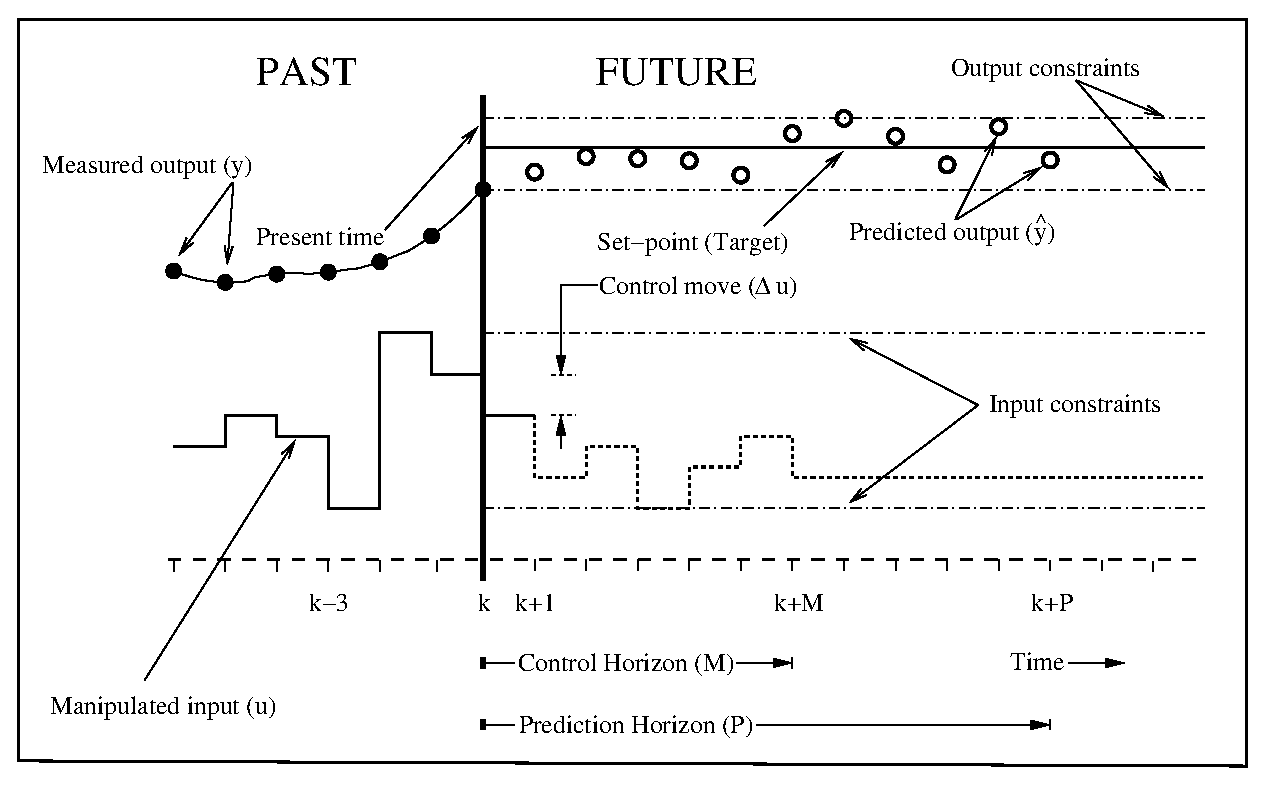
\includegraphics[width=5in]{mpc.eps}
\end{center}
\renewcommand{\baselinestretch}{1}
\small\normalsize
\begin{quote}
\caption[Figure with caption indented]{This figure caption is indented and single-spaced.  Comparison between the experimental measurements \cite{hart1} (black), the random initial condition NLSE model excluding phase noise (dashed curves) and the stochastic phase noise NLSE model (solid curves) showing the first- and second-order sideband evolution as a function of fiber length for P$_{0} = 5.5$\,W, $\Omega = 366$\,GHz, $\Delta\nu = 0.5$\,GHz, $\gamma = 0.019$\,W$^{-1}$m$^{-1}$, and $\beta^{(2)} = 55$\,ps$^2$/km: dynamical evolution of the: (a) power in the first-order blue-shifted sideband, (b) power in the first-order red-shifted sideband, (c) fluctuations in the first-order blue-shifted sideband, (d) fluctuations in the first-order red-shifted sideband, (e) power in the second-order blue-shifted sideband, (f) power in the second-order red-shifted sideband. \label{fig:fig27}}
\end{quote}
\end{figure}
\renewcommand{\baselinestretch}{2}
\small\normalsize

The first figure is Fig.\ref{fig:fig27}.   Please note that the figure label should be placed inside the figure caption.
\newpage

The next figure is placed landscape.  It is Fig.~\ref{fig:mpc}.

\begin{landscape}
\renewcommand{\baselinestretch}{1}
\small\normalsize
\begin{quote}
\begin{figure}
\begin{center}
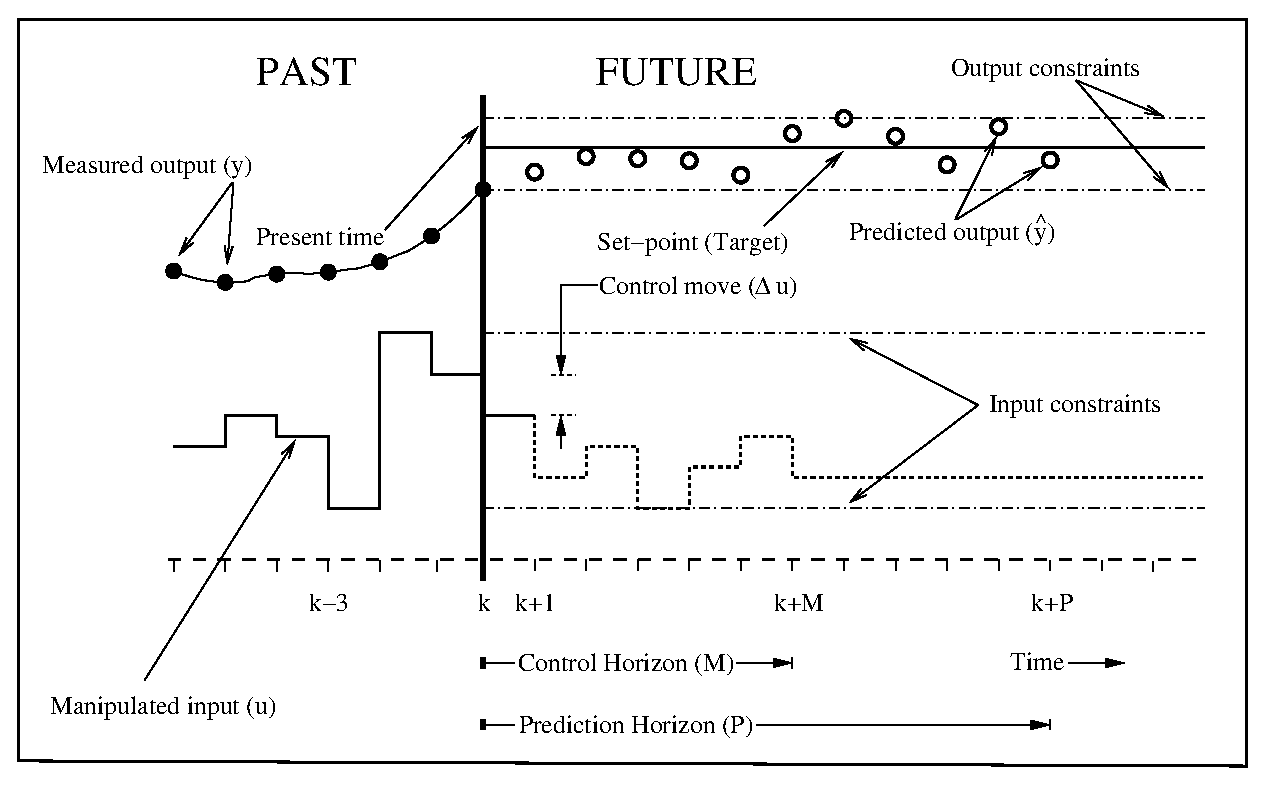
\includegraphics[width=8.2in]{mpc.eps}
\end{center}
\caption{Schematic illustrating receding horizon control.
\label{fig:mpc} }
\end{figure}
\end{quote}
\renewcommand{\baselinestretch}{2}
\small\normalsize
\end{landscape}

This is a my second figure which was placed landscape.  Although I have used the same figure, I have renamed the label to fig:mpc-1.  The second figure now becomes Figure~\ref{fig:mpc-1}.
\begin{landscape}
\renewcommand{\baselinestretch}{1}
\small\normalsize
\begin{quote}
\begin{figure}
\begin{center}
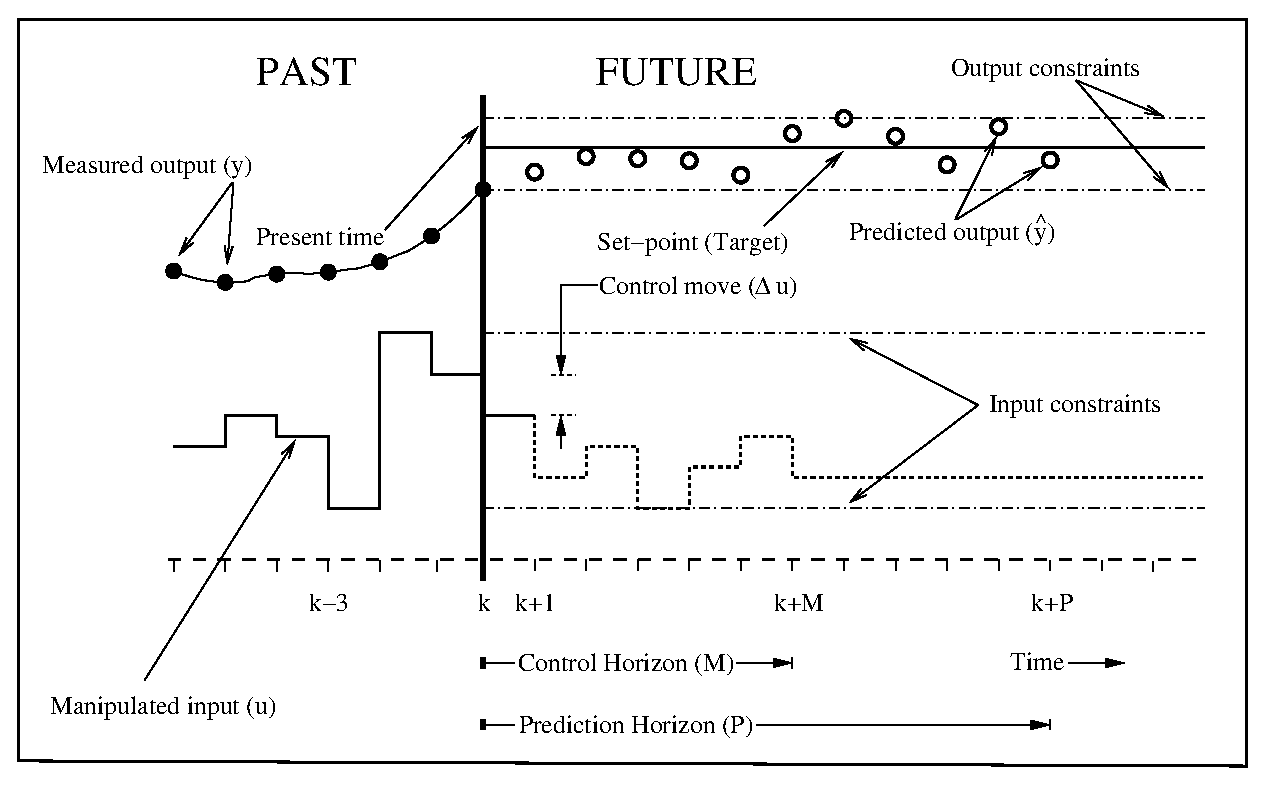
\includegraphics[width=8.2in]{mpc.eps}
\end{center}
\caption[Figure placed landscape on page]{Schematic illustrating receding horizon control. \label{fig:mpc-1}}
\end{figure}
\end{quote}
\renewcommand{\baselinestretch}{2}
\small\normalsize
\end{landscape}

\subsection{Numbering Figures}

If you wish your figures to be numbered 1-100 without any reference to the chapter (e.g., Figure 1.1, 2.1, etc.), change the first line of your mainthesis.tex file to read \begin{verbatim}"\documentclass[12pt]{thesis-2}".\end{verbatim}

\subsubsection{This is a Subsubsection}

This is my first subsubsection in Chapter 1.


\section[Short Titles]{Short Titles in the Table of Contents, List of Figures, or List of Tables}

The Table of Contents, List of Figures, or List of Tables usually show the entire title of a section, subsection, etc. or table, or the entire caption of a figure.  If you put a short title in square brackets after \begin{verbatim} \section, \table, or \figure, \end{verbatim} the short title will show in your Table of Contents or lists.

\renewcommand{\baselinestretch}{1}
\small\normalsize

\begin{verbatim}
\section[Short Title]{Title of Section}
\subsection[Short Title]{Title of Subsection}
\end{verbatim}

or when using a caption in a figure or table
\begin{verbatim}
\caption[Short Caption]{Full text of the caption.}
\end{verbatim}

\renewcommand{\baselinestretch}{2}
\small\normalsize


\section{Figures on Text Page}

Normally figures in the thesis are placed on a page by themselves.  The following figure is placed on the page with text before and after the figure by adding [!!h] after \begin{verbatim} \begin{figure}[!!h] \end{verbatim}.  Please note that the figure label is placed within the caption.

\renewcommand{\baselinestretch}{1}
\large\normalsize

\begin{verbatim}
\begin{figure}[!!h]
 \begin{center}
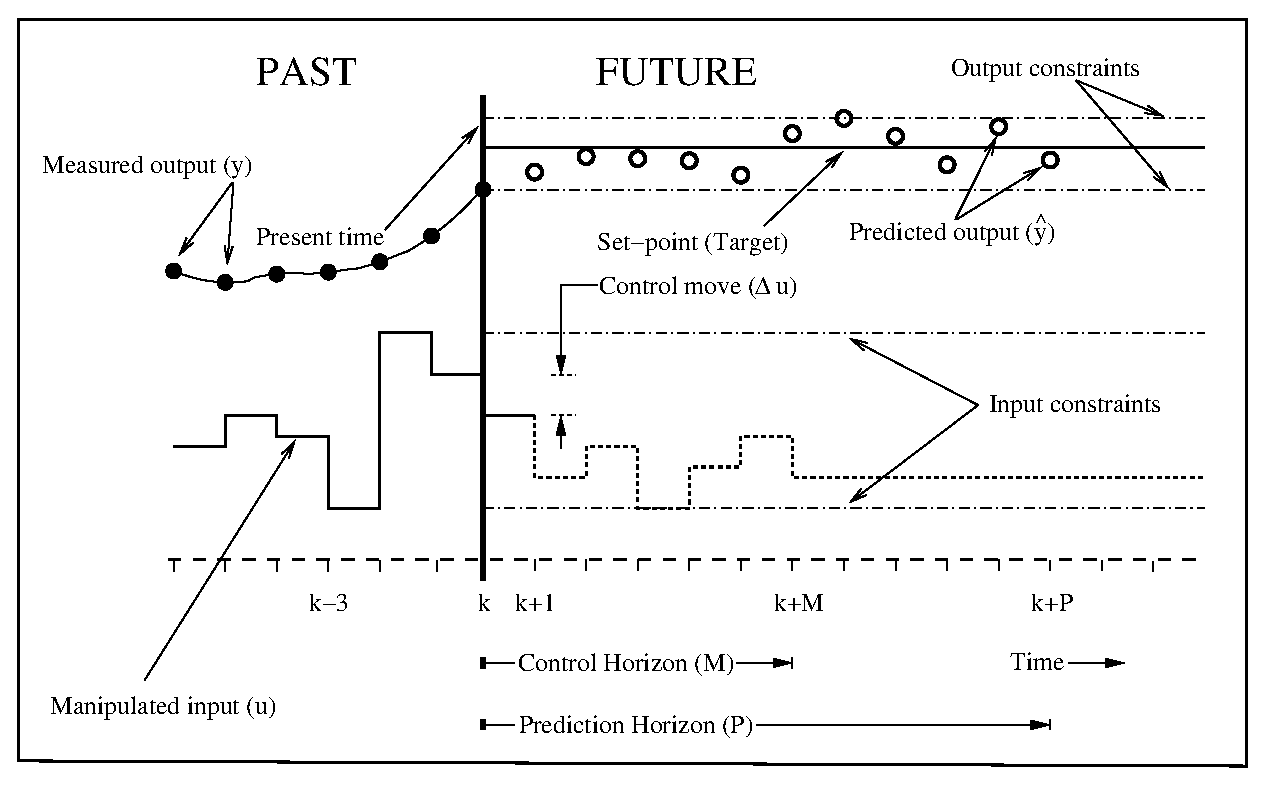
\includegraphics[width=5in]{mpc.eps}
\end{center}
\caption[Short title]{Schematic illustrating receding horizon control.
\label{fig:mpc-2}}
\end{figure}
\end{verbatim}

\begin{figure}[!!h]
 \begin{center}
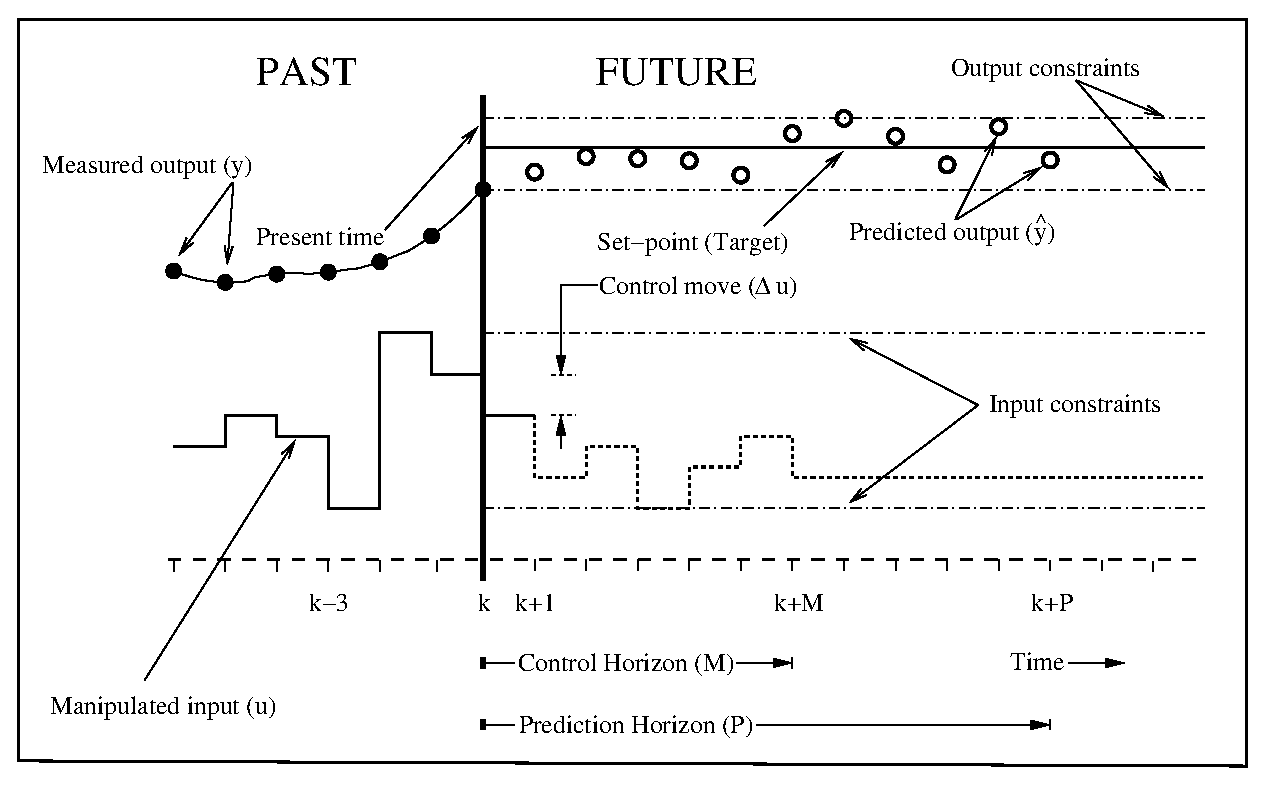
\includegraphics[width=5in]{mpc.eps}
\end{center}
\caption{Schematic illustrating receding horizon control. \label{fig:mpc-2}}
\end{figure}

\renewcommand{\baselinestretch}{2}
\large\normalsize

This does not necessarily mean that the text before and after the figure will be exactly what you want.  Remember Latex will place the figure where it will fit on the page the best.   The previous figure is Figs.~\ref{fig:mpc-2}.

\section{Wrapping Text around Figure}


\renewcommand{\baselinestretch}{1}
\begin{wrapfigure}{r}{0.4\textwidth}
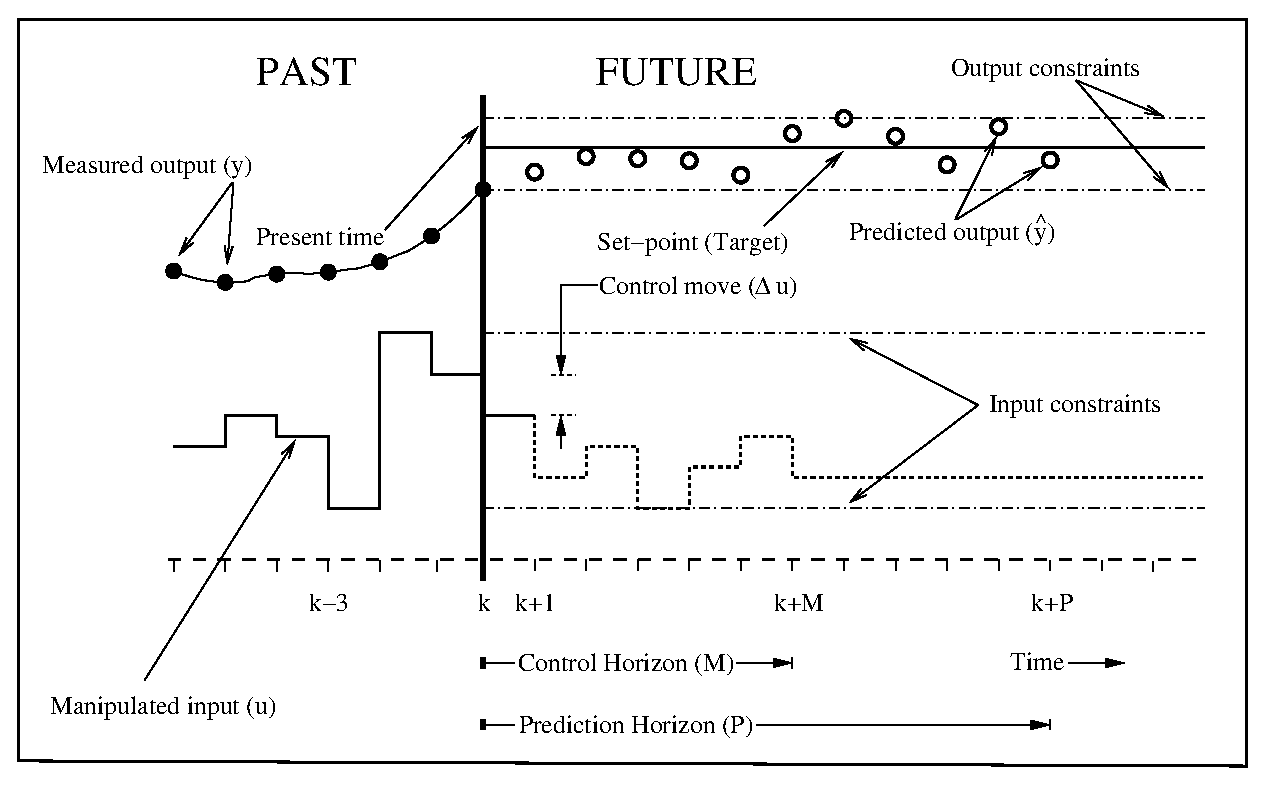
\includegraphics[width=0.4\textwidth]{mpc.eps}
\caption{ Text wrap around figure. \label{fig:test}}
\end{wrapfigure}

\renewcommand{\baselinestretch}{2}
\large\normalsize

By way of summary, at the end of the activity, I reminded the class of what we'd done:  by considering relatively nearby galaxies whose distance we had measured by some other means, we were able to establish a relationship locally between redshift and distance.
By way of summary, at the end of the activity, I reminded the class of what we'd done:  by considering relatively nearby galaxies whose distance we had measured by some other means, we were able to establish a relationship locally between redshift and distance.
By way of summary, at the end of the activity, I reminded the class of what we'd done:  by considering relatively nearby galaxies whose distance we had measured by some other means, we were able to establish a relationship locally between redshift and distance.
By way of summary, at the end of the activity, I reminded the class of what we'd done:  by considering relatively nearby galaxies whose distance we had measured by some other means, we were able to establish a relationship locally between redshift and distance.  See Fig.~\ref{fig:test}.


\section{LaTeX -- A Typesetting Program}

A 13-page explanation of some of the features of LaTeX can be downloaded from http://www.jgsee.kmutt.ac.th/exell/General/LaTeX.html.


\section{Using Bibtex}

Using Bibtex with Latex documents is not difficult.  The bulk of the work is organizing your bibtex file, which is a data base compiled by you of the articles, books, etc. which you use in the bibliographies or reference sections of your publications.

I have linked several files to this webpage, which will be helpful when you are using Bibtex.  These files can be downloaded from \newline
http://www.ireap.umd.edu/ireap/theses/bibtex.  Please read the file "BibtexInstructions.pdf".  The first two pages explain how to set up and run Bibtex; the remaining pages were taken from a published article and show how the references were cited in the .tex file.   The files BibtexInstructions.tex, Galactic.bib, Dottie.bib are the original .tex files used for BibtexInstructions.pdf.  The file BibtexSamples.tex contains examples of the information needed for the various publications you wish to reference (e.g., articles in refereed journals, books, unpublished articles, conference proceedings, etc.).

If you have questions concerning Bibtex, please contact me at 301-405-4955 or dbrosius at umd.edu.

\section{Using Natbib}

Another option of citing references in the bibliography is using
Natbib instead of Bibtex.  You must still create a bibtex file, as
noted above.  The command "backslash cite" cannot be used with
natbib; instead "backslash citet" and "backslash citep" must be
used. "backslash citet" is used to show references in the text
(e.g., Eq.\ 8 in Reiser,1996 shows ...); "backslash citep" is used
in the parenthetical (e.g., Eq.\ 8 (Reiser, 1996) shows ...).

\begin{verbatim}
Add in preamble -- \usepackage[option]{natbib}  --  A list of
options to be used with Natbib can be found at
"http://merkel.zoneo.net/Latex/natbib.php".

Add at bottom of mainthesis.tex file --
\bibliography{name of your bibtex file}
\bibliographystyle{plainnat, abbrnat, or unsrtnat} (I usually use
unsrtnat)

\end{verbatim}

Typesetting:   pdflatex, Bib, pdflatex, pdflatex

I use MikTex with WinEdt.

The reference sheet for natbib usage can be found at \newline "http://merkel.zoneo.net/Latex/natbib.php".

\section{APS Physical Review Style and Notation Guide}

The following style guide may be downloaded from The American Physical Society at http://forms.aps.org/author/styleguide.pdf:  Physical Review Style and Notation Guide, published by The American Physical Society, compiled and edited by Anne Waldron, Peggy Judd, and Valerie Miller, February 1993.  It may be old, but it is very useful.



%%Chapter 3

\renewcommand{\thechapter}{3}

\newcommand{\swave}[0]{$\it{s}$-wave}
\newcommand{\pwave}[0]{$\it{p}$-wave}
\newcommand{\K}{$^{40}\rm{K}$}
\newcommand{\Rb}{$^{87}\rm{Rb}$}
\newcommand{\us}{$\rm{\mu s}$}
\newcommand{\mT}{$\rm{mT}$}
\newcommand{\ez}{$\bf{\mathit{e}_z}$}
\newcommand{\ex}{$\bf{\mathit{e}_x}$}
\newcommand{\um}{$\rm{\mu m}$}
\renewcommand{\thefootnote}{\arabic{footnote}}



\chapter{Direct measurement of a Feshbach resonance in \K{} via observation of \textit{s}-wave scattering}

\section{Introduction}
Feshbach resonances are widely used for tuning the interaction strength in ultracold atomic gases. They have been particularly instrumental in the study of interactions and interaction-dependent processes in cold Fermi gases. In contrast to atomic Bose-Einstein condensates (BECs), where even weak interactions play a crucial role, for example giving rise to their characteristic Thomas-Fermi density profiles \cite{KetterleBEC},  interractions must compete with the Fermi energy before becoming relevant. Practically speaking, the density of Fermi clouds is typically $\sim$1000 times less than that of BECs \footnote{This is not the case for recently realized erbium and dysprosium DFGs \cite{Aikawa14,Lu12}, where strong dipolar interactions are present.}, making it necessary to enhance the strength of interactions in order to observe significant interaction effects\cite{KetterleDFG}. The tunability of interactions provided by Feshbach resonances has allowed for creation of molecular Bose-Einstein condensates from Fermi gases \cite{Greiner03,Zwierlein03, Jochim03} as well as observation of the phase transition from the Bardeen-Cooper-Schrieffer (BCS) superconduting regime to the BEC regime at sufficiently low temperatures \cite{Bartenstein04, Bourdel04, Zwierlein04, Regal04}.
\par A Feshbach resonance occurs when a diatomic molecular state energetically approaches the two-atom continuum \cite{Chin10, Timmermans99}. In experiment, the relative energy of the free atomic states in two hyperfine sublevels and the molecular state is defined by a bias magnetic field. Consequently, the Feshbach resonance can be accessed by changing the bias field. In the simple case where there are no inelastic two-body channels, such as for the \K{} resonance discussed in this work, the effect of the resonance on the scattering length between two free atoms is \cite{Chin10}
\begin{equation}
a(B)=a_{\rm{bg}}\left(1-\frac{\Delta}{B-B_0}\right),
\label{feshbachEq}
\end{equation}
where $a_{\rm{bg}}$ is the background scattering length, $\Delta$ is the width of the resonance, and $B_0$ is the field value at which the resonance occurs. The scattering length diverges at the resonance.
\par  The exact value of the resonant field $B_0$ is difficult to calculate analytically and is commonly computed via numerical models based on experimental input parameters \cite{Tiesinga93, Lysebo09, Gao11} or determined experimentally \cite{Inouye98, Cornish00}. Many experimental techniques have been used to characterize Feshbach resonances, including the observation of atom loss due to three-body inelastic scattering, measurement of re-thermalization timescales, and anisotropic expansion of the cloud upon release from a confining potential, all of which infer the elastic scattering cross section from collective behavior of the cloud \cite{Regal03,OHara02,Monroe93}.
\par Here we used direct scattering as a primary probe of the location and width of a Feshbach resonance. We collided pairs of ultra-cold Fermi gases and directly imaged the resulting \swave{} scattered atoms as a function of magnetic field strength. This allowed us to observe the enhancement in scattering without relying on proxy effects. We measured the fraction of atoms scattered during the collision, and from this fraction deduced the resonant magnetic field  and the width of the resonance.
%A similar technique has been used to characterize impurity scattering in BECs \cite{Chikkatur00}.
%\par The techniques developed in this experiment for observing Fermion scattering can be extended to engineering higher order partial wave interactions, as has been done for bosons \cite{Williams2012}.

In our dilute DFGs, even with the resonant enhancement of the scattering cross section, only a small fraction of the atoms scattered as the clouds passed through each other. This made direct detection of scattered atoms difficult due to detection uncertainty that disproportionately affected regions of low atomic density. To optimize the signal-to-noise ratio (SNR) for low atom numbers, we absorption imaged with fairly long, high-intensity pulses --- a non-standard regime, where the atoms acquired a velocity during imaging and the resulting Doppler-shift was non-negligible.  Simulation of the absorption imaging process was necessary for an accurate interpretation of these images. Using the simulation-corrected images, we extracted the fraction of atoms scattered in our collision experiment.

This paper is divided into two parts. In the first, we study absorption imaging in the presence of a significant time-dependent Doppler shift and show how we use our results to interpret data. In the second, we describe our \swave{} scattering experiment and extract a measure of the location and width of the Feshbach resonance in \K{}.

\section{Experimental setup}
In this section we describe our Fermi scattering experiment. We collided two counter-propagating \K{} clouds and observed the resulting \swave{} halo of scattered atoms.  We measured the dependence of the scattered atomic fraction on the bias magnetic field in the vicinity of the Feshbach resonance. We used this data to extract the location of the magnetic fields resonance of 20.206(15) \mT{} and a width of 1.0(5) \mT{}, similar to the accepted values of 20.210(7) \mT{} and 0.78(6) \mT{} \cite{Regal04}.

We prepared clouds of cold \K{} atoms in a hybrid \K{} and \Rb{} apparatus, previously described in \cite{Williams13, Lin09, KarinaThesis}. We used a Zeeman slower to slow both species before capturing in a magneto-optical trap (MOT). After 7 s seconds of MOT loading \K{} followed by 1.5 s of loading both \K{} and \Rb{}, we cooled both species in optical molasses for 2 ms. We optically pumped both species into their maximally stretched magnetically trappable states, $\ket{F=9/2, m_F=9/2}$ for \K{} and $\ket{F=2,m_F=2}$ for \Rb{}. Both species were then loaded into a quadrupole magnetic trap with a $\approx$ 7.68 mT/cm gradient along \ez, and cooled evaporatively via forced RF evaporation, sweeping the RF frequency from 18 MHz to 2 MHz in 10 s. The magnetic trap was plugged by a $\lambda =$ 532 nm beam, tightly focused to $\approx$ 30 \um{} and $\approx$ 5 W in power, providing a repulsive potential around the zero field point to prevent Majorana losses. Since the \K{} atoms were spin polarized and therefore only interacted by the strongly suppressed \pwave{} interactions, they re-thermalized only due to sympathetic cooling with \Rb{} atoms.

We then loaded the atoms into a crossed optical dipole trap, provided by a 1064 nm fiber laser, and continued evaporative cooling by slowly ramping down the dipole trap to trap frequencies of $(\omega_x,\omega_y,\omega_z)/2\pi =(39, 42, 124)$ Hz in the three spatial directions, while also turning off the quadrupole field. We then used adiabatic rapid passage (ARP) to transfer the \Rb{} atoms from the $\ket{F=2, m_F=2}$ state to the  $\ket{F=1, m_F=-1}$ absolute ground state via 6.8556 GHz microwave coupling (20.02 MHz from the zero field resonance) followed by a magnetic field sweep from -0.469 mT to -0.486 mT in 50 ms. This state was chosen to minimize spin changing collisions with \K{} atoms during any further evaporation \cite{BestThesis}.  We then briefly applied an on-resonant probe laser, ejecting any remaining \Rb{} atoms in the $F=2$ manifold from the trap. We again used ARP to transfer the \K{} atoms into the $\ket{F=9/2,m_F=-9/2}$ state by using a 3.3 MHz rf field and sweeping the bias magnetic field from -0.518 mT to -0.601 mT in 150 ms.

Following the state transfer, we had two versions of the protocol \--- one for approaching the Feshbach resonance from higher fields and one for approaching it from lower fields. For approaching the resonance from lower fields, we proceeded by ramping the bias magnetic field to 19.05 mT, turning on a 42.42 MHz RF field, and then sinusoidally modulating the bias field at 125 Hz for 0.5 s, with a 0.14 mT amplitude, decohering the \K{} state into an equal mixture of $\ket{F=9/2,m_F=-9/2}$ and $\ket{F=9/2,m_F=-7/2}$. For approaching the resonance from higher fields, the same was done at a bias field of 21.71 mT and an RF frequency of 112.3 MHz. The depolarization allowed the \K{} atoms to interact and re-thermalize, allowing us to further evaporate in the dipole trap \cite{DeMarco99}. Since \Rb{} is heavier than \K{}, we were able to evaporate the \K{} atoms past the point where \Rb{} atoms were no longer suspended against gravity and had been completely removed.  These hyperfine states of \K{} were then used to study their Feshbach resonance.
\par After evaporation, we ramped the bias field in a two-step fashion to the desired value $B$ near the Feshbach resonance. We approached the field using a large pair of  coils in Helmholtz configuration (0.19 mT/A) to bring the magnetic field to a setpoint 0.59 \mT{} away from $B$,  $B-0.59$ \mT{} when approaching from below and $B+0.59$  \mT{} from above. We held the atoms at this field for 100 $\rm{ms}$ to allow the eddy currents induced by the large coils to settle, and then used a lower inductance (0.017 mT/A) set of Helmholtz coils to quickly change the field the remaining 0.59 \mT{}. This allowed us to study the resonance from both sides without the added losses associated with going through the resonance \cite{Chin10}.

Once at the intended bias field, we split the cloud into two spatially overlapping components with opposing momenta  and observed scattering as they moved through each other and separated. These counterpropagating components were created using an  8$E_{\rm{L}}$ deep near resonant ($\lambda_{\rm{L}}$=766.704 nm) 1-d retro-reflected optical lattice, where $E_{\rm{L}}=\hbar^2 k_{\rm{L}}^2/2m_{\rm{K}}$ is the lattice recoil energy and $\hbar k_{\rm{L}}=2\pi \hbar/ \lambda$ is the recoil momentum. We rapidly pulsed this lattice on and off with a double-pulse protocol \cite{Wu05, Edwards10}. The pulse sequence was optimized to transfer most of the atoms into the $\pm 2 \hbar k_{\rm{L}}$ momentum states. Since the initial Fermi gas had a wide momentum spread (in contrast to a BEC, which has a very narrow momentum spread), and the lattice pulsing is a momentum dependent process  \cite{Wu05}, not all the atoms were transferred into the target momentum states. We optimized our pulse times to minimize the atoms remaining in the zero momentum state. The optimized pulse times were 23 \us{} for the first pulse, 13 \us{} off interval, and 12 \us{} for the second pulse \cite{Edwards10}.

We then released the atoms from the trap and allowed 1 ms for the two opposite momentum states within the cloud to pass through each other, scattering on the way. For the data taken coming from below the Feshbach resonance, we then simply ramped down the field and imaged the atoms. For the data taken coming from above the Feshbach resonance, we ramped the field back up, retreating through the resonance if it had been crossed and thereby dissociating any molecules that were created, and then quickly ramped the field back down and imaged the atoms. We used a 40 \us{} imaging pulse with $I_0/I_{\rm{sat}}\approx 0.6$ at the center of the probe laser.

The total time-of-flight, the time from the moment the atoms were released from the trap to when they were imaged, was $t_{TOF}=6.8$ $\rm{ms}$. In such an image, the observed atomic position is determined by the initial velocity upon release from the trap, along with the time-of-fligt time $t_{TOF}$. Therefore, this technique measures the momentum and not the position distribution of the atoms.

The magnetic fields produced by our coils in the regime of interest were independently calibrated by rf-spectroscopy. We prepared \K{} atoms in the $\ket{F=9/2, m_F=-9/2}$ state and illuminated them with and rf-field with some frequency $\nu_{rf}$. We then ramped our high-inductance coils to variable set points, followed by an adiabatic 250\us{} ramp of 2.84 mT in the lower inductance coils. We then used Stern-Gerlach and observed the fractional population in the $\ket{F=9/2, m_F=-9/2}$  and $\ket{F=9/2, m_F=-7/2}$ states as a function of the high-inductance coil current. We fit the fractional population curve to a Gaussian, and considered the center of the fit to be on-resonant, with an uncertainty given by the Gaussian width. We used the Breit-Rabi formula to determine the resonant field value at $\nu_{rf}$. We did this for 5 different rf frequencies, and acquired a field calibration with an uncertainty of 0.3 mT, which was included in the listed uncertainty on the center field of the Feshbach resonance.


\section{Methods}

We first processed each image by comparing the obsereved $OD$s to simulations taking into account the recoil induced detuning as described in Sec. \ref{sec:2}. An example of images before and after processing are shown in Fig. \ref{fig:SampleCorrection}.  To improve the signal and mitigate our shot to shot number fluctuations, we took 15 nominally identical images for each data point.
\begin{figure}
	\subfigure[]{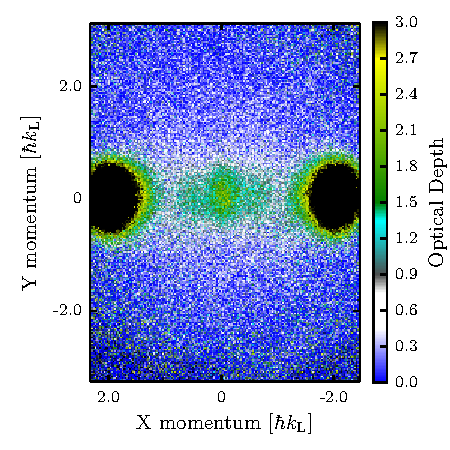
\includegraphics{Chapter3 Figures/figure10a.pdf}}
	\subfigure[]{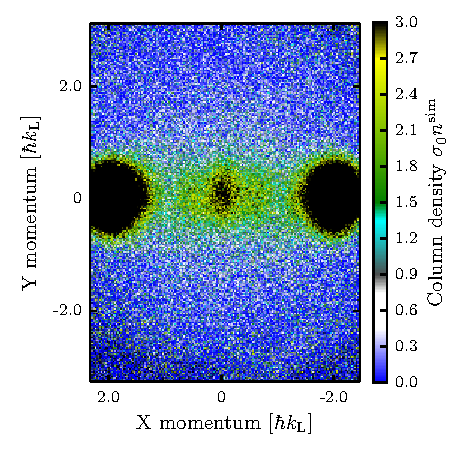
\includegraphics{Chapter3 Figures/figure10b.pdf}}
\caption{An example of our absorption image after 6.8 ms TOF. The 1-D lattice imparts momentum along \ex{}. The two large clouds on the left and right are the atoms in the $\pm 2 k_{\rm{L}}$ momentum orders that passed through each other unscattered. The smaller cloud in the center is the atoms that remained in the lowest band of the lattice after pulsing, and thus obtained no momentum. The thin spread of atoms around these clouds is the atoms that underwent scattering.   This image was taken coming from below the Feshbach resonance at 20.07  \mT{}. (a) Raw optical depth, (b) atomic column density obtained by comparing to simulated $OD$s, $\sigma_0 n^{\rm{sim}}$ }
\label{fig:SampleCorrection}
\end{figure}

We counted the fraction of atoms that experienced a single scattering event for each of the fifteen images at a given bias magnetic field. Single scattering events are easily identified, as two atoms that scatter elastically keep the same amplitude of momentum, but depart along an arbitrary direction. Therefore, an atom traveling at $2 \hbar k_{\rm{L}}$ to the right that collides elastically with an atom traveling at $-2 \hbar k_{\rm{L}}$ to the left will depart with equal and opposite momenta $2 \hbar k_{\rm{L}}$ at an arbitrary angle, and in a time of flight image such atoms will lie in a spherical shell, producing the scattering halo pictured in Fig. \ref{fig:halo}(a).
\begin{figure}
	\subfigure[]{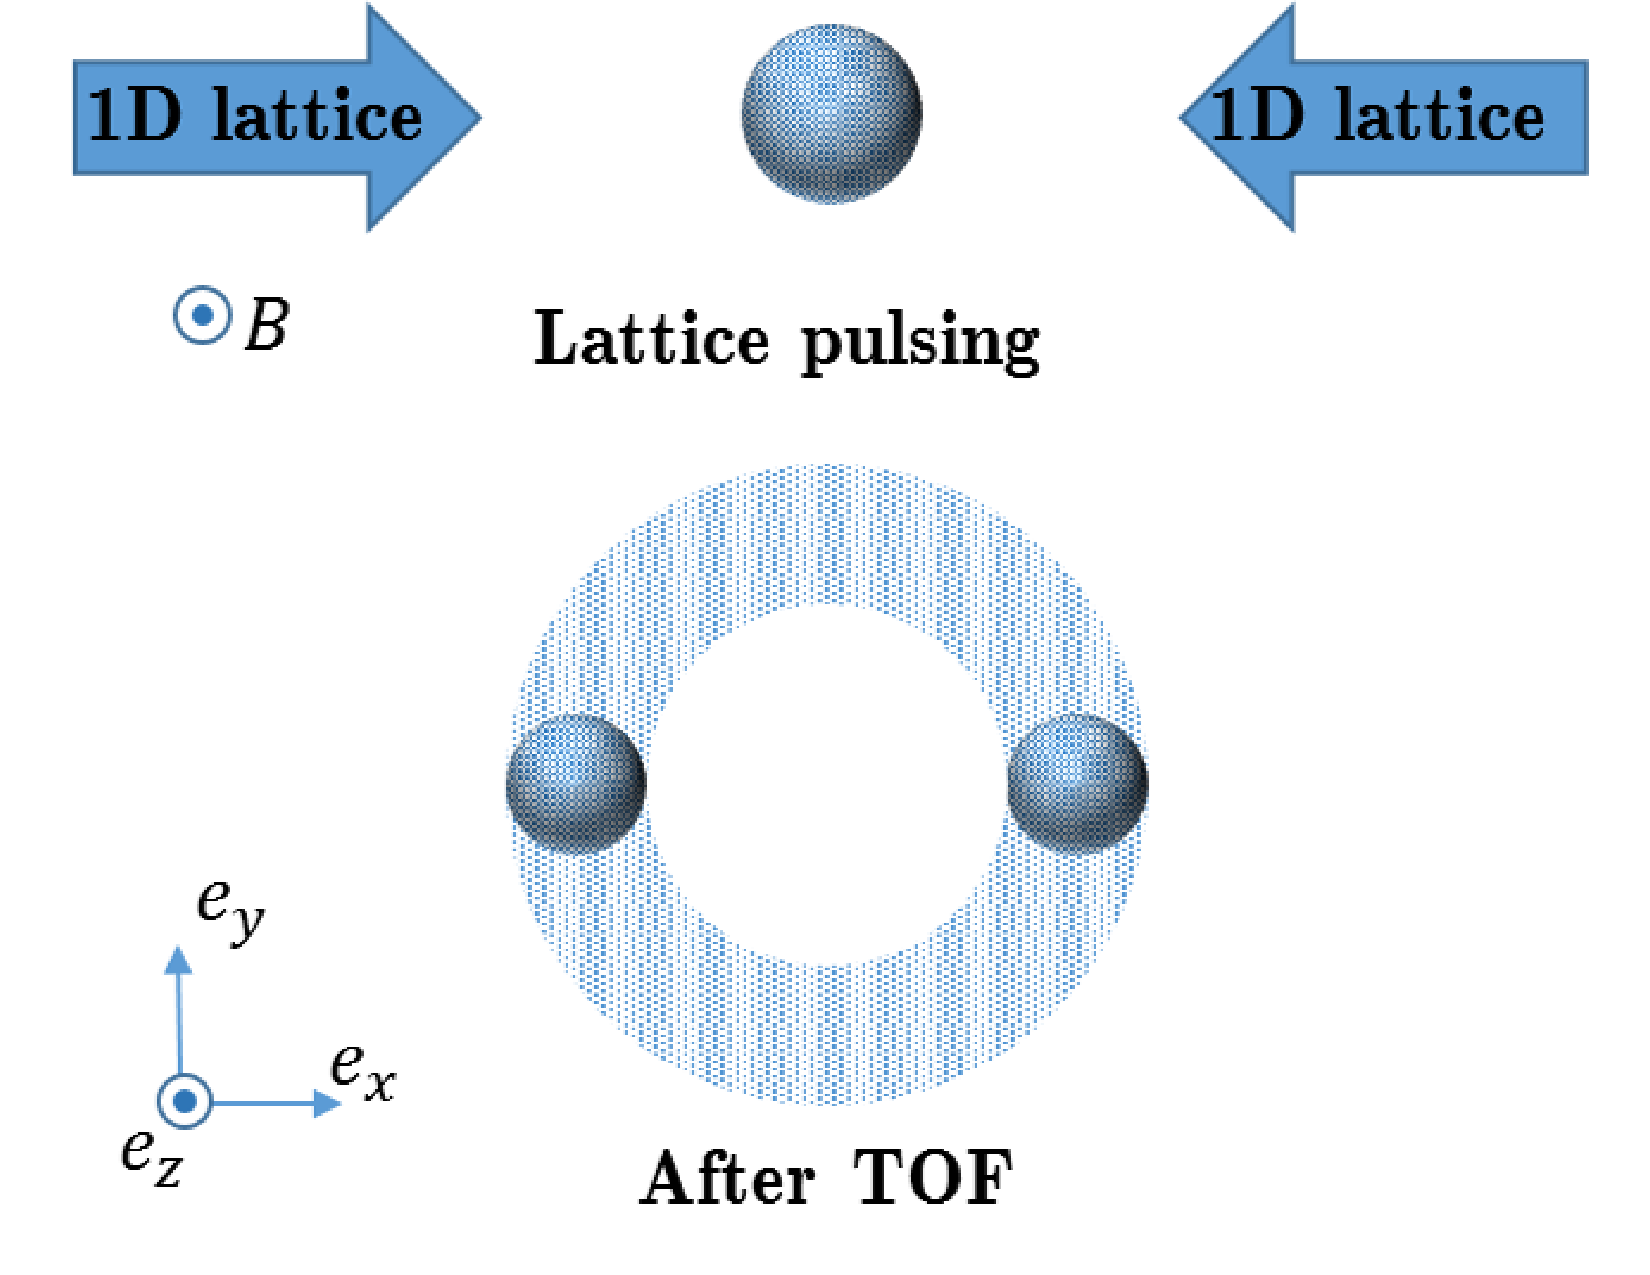
\includegraphics[scale=0.25]{Chapter3 Figures/Picture12.pdf}}
	\subfigure[]{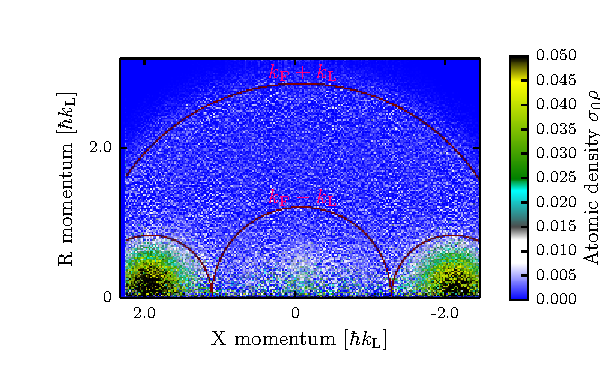
\includegraphics{Chapter3 Figures/figure12b.pdf}}
\caption{(a) Our experimental setup. After time of flight, the two clouds traveling along $\pm \hat{e}_x$ directions have separated and the atoms that underwent a single scattering event were evenly distributed in a scattering halo around the unscattered clouds. The 1-D lattice defined the axis of cylindrical symmetry. (b) Inverse Abel transformed image. The atoms within the Fermi momentum $k_F$ of each unscattered cloud center are in the unscattered region and counted towards the total unscattered number. The atoms outside the radius $ k_{\rm{L}}-k_{\rm{F}}$ but inside $k_{\rm{L}}+k_{\rm{F}}$ but outside the unscattered region are counted towards the number of single scattered atoms.   }
\label{fig:halo}
\end{figure}

Absorption images captured the integrated column density along \ez{}, a projected 2D atomic distribution. To extract the radial dependence of the 3D distribution from the 2D image, we performed a standard inverse Abel transform. The inverse Abel transform assumes cylindrical symmetry, which was present in our case, with the axis of symmetry along \ex{}, defined by the lattice. We neglect the initial asymmetry of the trap, as during time-of-flight the atoms travel far beyond the initial extent of the cloud  $(r_x,r_y,r_z)\approx$ (45,48,15) \um{}, while the cloud width after TOF is $\approx$ 82 \um in each direction. We thus obtained the atomic distribution $\rho(r,\theta)$ as a function of $r$, the radial distance from the scattering center, and $\theta$, the angle between $r$ and symmetry axis \ex{}, integrated over $\phi$, the azimuthal angle around the $x$ axis.

We then extracted the number of scattered atoms $N_{\rm{scat}}$ as a fraction of the total atom number $N_{\rm{tot}}$ for each image, as shown in Fig. \ref{fig:halo}(b). The unscattered atom number was the number of atoms in the two unscattered clouds. The number of atoms that underwent a single scattering event was the number of atoms outside the Fermi radius of the unscattered clouds, but inside the arc created by rotating the Fermi momentum $k_{\rm{F}}$ around the original center of the cloud (red arcs in Fig. \ref{fig:halo}(b)). For both the scattered and unscattered numbers, we accounted for atoms that fell outside the field of view of our camera by multiplying the counted atom number by a factor of the total area as defined by the radii divided by the visible area on the camera. The atoms in the center region were not counted as they were originally in the zero momentum state and could not contribute to the scattering halo under study.

We fit the fraction of scattered atoms versus the total atom number for each of the 15 images taken at the same bias magnetic field to a line constrained to be zero at zero. The slope of this fit was taken to be the value of $N_{\rm{scat}}/N_{\rm{tot}}^2$ at that bias magnetic field, and the variance of the fit gave the uncertainty on that data point. This uncertainty reflected our shot to shot number fluctuations, which produced variable atomic densities and thus influence the scattered fraction. 

We then deduced the resonant field value $B_0$ and width of the resonance  $\Delta$, the parameters in Eq. (\ref{feshbachEq}).  Since we were in the low energy regime (the atomic momentum was much smaller than the momentum set by the van der Waals length $k_{\rm{L}}+k_{\rm{F}}\ll1/l_{\rm{vdW}}$, and we were well below the p-wave threshold temperature \cite{DeMarco99}), the scattering cross-section was given by $\sigma=4\pi a^2$.

The scattering cross-section $\sigma$ gives the probability $P_{\rm{scat}}=\sigma N/A$ that a single particle will scatter when incident on a cloud of atoms with a surface density of $N/A$, where $A$ is the cross-sectional area of the cloud and $N$ is the number of atoms in the cloud. In our case, each half of the initial cloud, with atoms number $N_{\rm{tot}}/2$, is incident on the other half. Thus, the number of expected scattering events is $N_{\rm{scat}}= (N_{\rm{tot}}/2) \sigma  (N_{\rm{tot}}/2)=\sigma N_{\rm{tot}}^2/4A$. Assuming $A$ is constant for all our data, we can define a fit parameter $b_0=4\pi a_{\rm{bg}}^2/4A$, where $a_{\rm{bg}}$ is the background scattering length. We can thus adapt Eq. (\ref{feshbachEq}) to obtain the fit function
\begin{equation}
\frac{N_{\rm{scat}}}{N_{\rm{tot}}^2}=b_0\left(1-\frac{\Delta}{B-B_0}\right)^2 + C.
\label{eq:fit}
\end{equation}
We found that our imaging noise skewed towards the positive, giving rise to a small background offset. We accounted for this in our fit by including a constant offset parameter $C$.


\section{Results}
Our final data is presented in Fig. \ref{fig:fittedFractions}. The red curve depicts a best fit of the model given in Eq. (\ref{eq:fit}). The fit parameters we extracted were $\Delta = 1(5)$  \mT{}, $B_0 = 20.206(15)$  \mT{}, $b_0 = 5(3)\times 10^{-3}$ and $C=8(1)\times 10^{-4}$. To obtain the fit, we used data taken by approaching the resonance from above for points above where we expected the resonance to be and data taken approaching the resonance from below for points below. We also excluded from the fit data points very near the resonance, as there the assumption $\sigma\rho\ll1$, where $\rho$ is the atom number per unit area, is no longer valid and the problem must be treated hydrodynamically.

The accepted values for the $^{40}K$ s-wave Feshbach resonance for the  $\ket{9/2,-9/2}$ and $\ket{9/2,-7/2}$ states are $B_0=20.210(7)$  \mT{} and $\Delta=0.78(6)$  \mT{} \cite{Regal04}, which is in good agreement with our findings. Some potential sources of systematic uncertainty that we did not account for include scattering with atoms that did not receive a momentum kick from the lattice pulsing or the impact of multiple scattering events.
\begin{figure}
	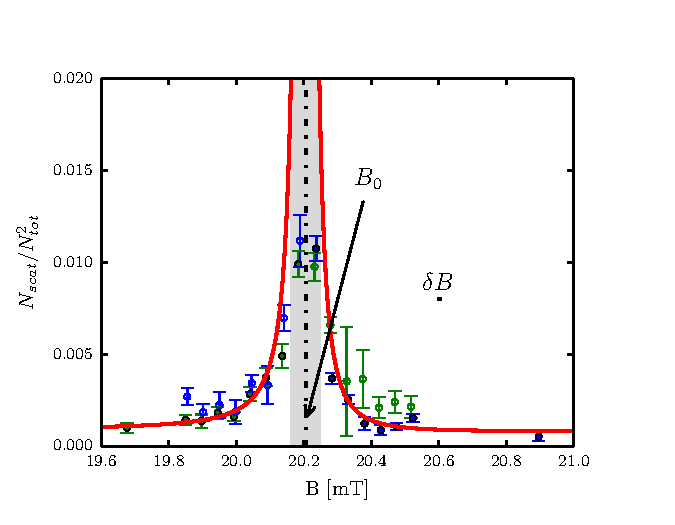
\includegraphics{Chapter3 Figures/figure11.pdf}
\caption{Normalized scattered population plotted versus bias field $B$. Green dots represent data taken coming from below the resonance, and blue dots represent the data taken coming from above the resonance. The red curve depicts the best fit, where data coming from above the resonance was used above the resonance and data coming from below the resonance was used below the resonance to create the fit; the unused data points are indicated by hollow dots. The regime where the scattering length is likely large enough for the atoms to behave hydrodynamically is shaded in gray, and data points in that area were also excluded from the fit. Resonant field value $B_0$ as found in this work and our systematic uncertainty in the bias magnetic field $\delta B_0$ are indicated.    }
\label{fig:fittedFractions}
\end{figure}
\section{Conclusion}
We studied the effects of recoil-induced detuning effects on absorption images and found an optimal imaging time of $\approx40$ \us{} for \K{} atoms for noise minimization after corrections. We use these results to observe s-wave scattering halos of the Fermi gas around the $\approx 20.2$ \mT{} Feshbach resonance and directly verified the resonance location and width. Our analysis can be used in any absorption imaging application where SNR optimization is critical.


%\titleformat{\chapter}
%{\normalfont\large}{Appendix \thechapter:}{1em}{}


%Chapter 2

\renewcommand{\thechapter}{2}


\chapter{Absorption imaging in the presence of strong recoil induced detuning}


\section{Near-resonant atom-light interaction}\label{chap:2sec:atomLight}

In this section, we will assume the atom can be treated as a two-level system: one with a ground and excited atomic state, with an energy difference of energy difference $\hbar\omega_0$. When such an atom, starting in the ground state, is illuminated by a laser beam with frequency $\hbar\omega_{\rm{L}}$, there are three kinds of transitions that occur: during aborption the atom aborbs a photon from the laser and goes from the ground to the excited state; during stimulated emission, the atom emits a photon into the field of the laser beam and jump from the excited to the ground state; during spontaneous emission, the atom decays to the ground state from the excited state with no help from the laser, emitting into a random vacuum mode. Stimulated emission results in coherent light co-propagating with the laser beam, while spontaneous emission results in light scattering incoherently in any direction. The rate of spontaneous emission from an excited state is given by the natural transition linewidth of the transition $\Gamma$. 

On timescales short compared to $1/\Gamma$, spontaneous emission can be ignored, and an atom undergoes coherent Rabi oscillations between the ground and excited states via cycles of absorption and stimulated emission\cite{LCT}. Taking $c_g$ and $c_e$ to be the time-dependent coefficients multiplying the eigenstate wavefuntions of the ground and excited state respectively, and assuming the atom starts in the ground state $c_g(t=0)=1$, the excited state population is given by
\begin{equation}
c_e(t)=-i\frac{\Omega}{\Omega'}sin\left(\frac{\Omega't}{2}\right)e^{-i\delta t/2},
\end{equation}
where $\Omega$ is the Rabi frequency given by $SOMETHING IN TERMS OF INTENSITY$, $\Omega'=\sqrt{\Omega^2+\delta^2}$ is the generalized Rabi frequency and $\delta=\omega_0-\omega_{\rm{L}}$ is the detuniong of the laser from atomic resonance. 

In the regime where spontaneous emission cannot be ignored, Rabi oscillations of each individual atom are intermittently interrupted by decay to the ground state. Averaging over an atomic ensamble, on the time scale of a single Rabi oscillation the overall excited state population reaches a steady state, and the rate of spontaneous emission becomes constant. Since during spontaneous emission the ejected photon can go into any vacuum mode, this process can be thought of as the scattering of photons by the atoms. This scattering rate is given by\cite{LCT}
\begin{equation}
\gamma_{\rm{sc}}= \frac{\Gamma}{2} \frac{I/I_{\rm{sat}}}{1+4(\delta/\Gamma)^2 +I/I_{\rm{sat}}},
\label{eq:scatrate}
\end{equation}
where $I_{\rm{sat}}$ is the saturation intensity. This is the intensity at which the timescale of spontaneous emission matches the Rabi oscillation rate, reducing the capacity for absorption of extra light.   


\section{Absorption imaging}

Absorption imaging takes advantage of the on-resonant interaction described in the previous section. An on or near-resonant laser beam ($\delta/\Gamma\ll 1$) is shined at the atoms, and the aborbed light acts to create a shadow in the shape of the atoms in the laser beam. This beam with the shadow is then imaged on a camera, in our case a CCD, as depicted in Figure \ref{fig:absorptionIntor}a (top). This is called the atom image, and the intensity distribution over the camera is denoted by $I_f(x,y)$, where the subscript f stands for final - the intensity after the light has encountered the atoms. To quantify the 'shadowed out' intensity, after the atoms have left the trap the same laser intensity is shined directly at the camera, as in Figure \ref{fig:absorptionIntor}a (bottom).   This is called the probe image, and the intensity distribution over the camera is denoted by $I_0(x,y)$, where the subscript 0 indicated initial - the intensity before the light had encountered the atoms.



%Absorption imaging measures the shadow cast by an atomic ensemble in an illuminating probe laser beam with angular frequency $\omega_{\rm{L}}$. 
%\par An absorption image is obtained by shining an on- or near-resonant probe beam ($\tilde{\delta}\ll1$) onto the atomic cloud. Some of the light is scattered by the atoms, and the unscattered light, $\tilde{I}_f(x,y)$, is imaged onto a camera, as depicted in Fig. \ref{fig:absorptionIntor}(a) (top). The probe light is reapplied with the atoms absent to calibrate the intensity $\tilde{I}_0(x,y)$ of light unaffected by the atoms (bottom).
\begin{figure}
	\subfigure[]{\includegraphics[scale=0.5]{"Chapter2 Figures/Picture1a"}}
	\subfigure[]{\includegraphics{"Chapter2 Figures/Picture1c".pdf}}
	\subfigure[]{\includegraphics[scale=0.55]{"Chapter2 Figures/Picture1b"}}
\caption{Absorption imaging. (a) Near resonant probe light illuminates the atoms, and the transmitted light (containing a shadow of the atoms) is imaged on the camera. A second image taken with no atoms provides a reference. (b)  The probe beam is partially absorbed as it traverses the cloud, and the intensity seen by atoms further along the imaging direction \ez{} is lowered.  (c) An atomic cloud illuminated by a probe light field absorbs photons from the probe and re-emits them in all directions. This process results in a net acceleration of the cloud in the direction of the probe light as well as diffusive spreading in the transverse directions.  }
\label{fig:absorptionIntor}
\end{figure}

To recover the atom number distribution encountered by the light, consider an atomic cloud with 3D density $\rho(x,y,z)$. Since we can only obtain 2D information from the camera, we can only hope to recover a 2D atomic column density $n(x,y)=\int\rho(x,y,z)\mathrm{d}z$. Focusing in on a single pixel of the camera, we can consider a single value of $I_0$ and $I_f$ to recover a local $n$. As the laser light propagates through the atomic cloud, the intensity of the light will diminish due to absorption. This absorption as a function of propagation direction $z$ can be expressed using the scattering rate equation Eq. \ref{eq:scatrate} as the number of photons scattered by the atoms (proportional to the atomic density times the scattering rate) times the photon energy $\hbar\omega_{\rm{L}}$:
\begin{equation}
\frac{d}{dz}\frac{I(z)}{I_{\rm{sat}}}=-\hbar\omega_{\rm{L}}\rho(z)\gamma_{sc}(z)=-\rho(z)\sigma_0\frac{I(z)/I_{\rm{sat}}}{1+4\delta^2 /\Gamma^2+I(z)/I_{\rm{sat}}},
\label{eq:dIdz}
\end{equation}
where the resonant scattering cross section is $\sigma_0=3\lambda_0^2/2\pi$, and $\lambda_0$ is the wavelength asociatted with atomic resonance. 

Integrating both sides of Eq. \ref{eq:dIdz}, we obtain
\begin{equation}
\sigma_0 n = \left(1+4\delta^2/\Gamma^2\right)\mathrm{ln}(I_0/I_f)+ \left(I_0-I_f\right)/I_{\rm{sat}}.
\label{eq2}
\end{equation}
The quantity $OD=ln(I_0/I_f)$ is called the optical depth of the cloud. When the probe intensity $I_0$ is much smaller than the saturation intensity, the second term in Eq. \ref{eq2} becomes negligible. Assuming further that the probe light is on resonance, $\delta=0$, the atomic column density becomes simply $\sigma_0 n=OD$. Figure \ref{fig:absorptionIntor}b shows a Gaussian atomic density distribution (top) and the resulting probe intensity as a function of position in the cloud (bottom). The intensity drops from its initial to final value gradually as it traverses the cloud.

However, there is an important effect that the above equations do not account for. Namely, as the atoms absorb light from the probe beam, they also get a momentum kick equal to the momentum of a photon during each collision $\hbar k_r=h/\lambda_L$ in the direction of propagation. It is true that the absorbed photon will then be re-emitted by the atom, inducing a loss of momentum, but since this happens through the process of spontaneous emission into a random vacuum mode, the average momentum kick acquired this way over many re-emissions will average to zero. On average, each photon absorbed will induce a change in velocity of the atom of $v_r=\hbar k_r/m$, where $m$ is the atomic mass, as depicted in Fig. \ref{fig:absorptionIntor}c. As the velocity of the atom changes, due to the Doppler effect, the apparent laser frequency will change as well. Therefore, even if the laser light is exactly on-resonant for a stationary atom, it will become off-resonant for longer imaging times, and Eq. \ref{eq:dIdz} will acquire a time dependence. For most experiments, this effect is small and can be neglected. However, if the imaging time becomes of order a recoil time $t_r$, a time after which the recoil-induced detuning $\delta$ becomes of order $\Gamma$, this effect becomes significant. We explore this effect in the following sections.  

%The intensity $\tilde{I}_f(x,y)$ is related to the number of atoms the light encountered. Consider the light as it travels along the imaging axis \ez{} through a 3D atomic density profile $\rho(x,y,z)$. We focus on a single pixel of the camera: sensitive to a single column of atoms $\rho(z)$ giving  $\tilde{I}_0$ and $\tilde{I}_f$. Our task is to invert the problem and obtain a column density $n = \int \rho\left(z\right) \,\mathrm{d}z$ given $\tilde{I}_0$ and $\tilde{I}_f$. As the light travels through a column of atoms, each atom scatters light according to Eq. (\ref{eq:scatrate}). Therefore, the atoms further along the imaging axis $z$ experience a reduced optical intensity due to attenuation of the laser field by the other atoms (Fig. \ref{fig:absorptionIntor}(b)). The intensity change from scattering as a function of $z$ is
%\begin{equation}
%\frac{d\tilde{I}(z)}{dz}=-\hbar\omega_{\rm{L}}\rho(z)\gamma_{sc}(z)=-\rho(z)\sigma_0\frac{\tilde{I}(z)}{1+4\tilde{\delta}^2 +\tilde{I}},
%\label{eq:dIdz}
%\end{equation}
%where $\sigma_0$ is the resonant scattering cross section. Integrating this equation yields a relation between the observed optical depth $OD=-\ln \left(I_f/I_0\right)$ and the atomic column density $n$ \cite{Reinaudi07} --- we call the column density deduced in this manner $\sigma_0 n^{\rm{(1)}}$:
%\begin{equation}
%\sigma_0 n^{\rm{(1)}} = \left(1+4\tilde{\delta}^2\right)OD+ \tilde{I}_0-\tilde{I}_f.
%\label{eq2}
%\end{equation}
%When the probe intensity is much smaller than the saturation intensity, $\tilde{I}_0\ll1$, and the probe light is on resonance, $\tilde{\delta}=0$, the right hand side of Eq. (\ref{eq2}) reduces to the optical depth \cite{Reinaudi07}, giving the simple relationship $\sigma_0 n^{\rm{(0)}}=OD$. 
%\par Equations (\ref{eq:dIdz})-(\ref{eq2}) neglect the atomic recoil momentum and its effect on the laser detuning \cite{Konstantinidis12}. When an atom absorbs a photon from the laser light field it acquires a momentum kick $\hbar  k_{\rm{r}}$ in the direction of the light field. The associated recoil velocity is $v_{\rm{r}}=\hbar k_{\rm{r}}/m$, where $m$ is the atomic mass and $\hbar k_{\rm{r}}= h/\lambda$ is the recoil momentum from the laser with wavelength $\lambda$. Each re-emitted photon imparts a similar recoil momentum $\bf{\mathit{p}_e}$, but over many scattering events this momentum distribution averages to zero. Therefore the atom  will acquire an average velocity per photon $v_{\rm{r}}$ along \ez{}. The variance of $\bf{\mathit{p}_e}$, however, is not zero, allowing the atoms to acquire some momentum transverse to the laser field. While we ignore this correction, it results in the reduction of spatial resolution in the final image and its effect on the atomic cloud is pictured in Fig. \ref{fig:absorptionIntor}(c).


\section{Recoil-induced detuning}

After absorbing a number of photons $N$, an atom will obtain a recoil velocity of $N v_{\rm{r}}$. Via the Doppler effect, this will result in a detuning $\delta=N k_{\rm{r}} v_{\rm{r}}$. This detuning will increase as more atoms are absorbed, and therefore depend on time, making the absorbed intensity also time dependent. We can generalize Eq. \ref{eq:dIdz} to include a time dependence on the detuning term and therefore also the intensity: 
\begin{equation}
\frac{d}{dz}\frac{I(z,t)}{I_{\rm{sat}}}=-\rho(z)\sigma_0\frac{I(z,t)/I_{\rm{sat}}}{1+4\delta(z,t)^2 /\Gamma^2+I(z,t)/I_{\rm{sat}}}. \label{eq3}
\end{equation}
The number of photons absorbed per atom will depend on the intensity lost, up until the current time, at that location. The detuning will therefore be proportional to the total number of photons lost up until time $t$ at that location, proportional to the absorbed intensity divided by the single photon energy $\hbar\omega_L$, divided by the number of atoms that participated in the aborption $\rho(z)$ times the detuning $ k_{\rm{r}} v_{\rm{r}}$:
\begin{equation}
\delta(t,z)=\frac{ k_{\rm{r}} v_{\rm{r}}}{\hbar\omega_L\rho(z)}\int_0^t\frac{dI(z,\tau)}{dz}\mathrm{d}\tau.
\label{eq4}
\end{equation}
These equations are interdependent, and cannot be in general solved analytically. 

Figure \ref{fig:expos}a shows the velocity and detuning as a function of position in space for three different imaging times, calculated numberically. All calculations in this chapter were done for a cloud of $^40\mathrm{K}$ atoms, as that is relevant to our experiment described in the next chapter. The resonant wavelength is $PUT ALL NUMBERS FOR K IN HERE$

\section{Perturbative treatment}
We can treat these equations perturbatively in time. To first order, we can set the detuning in Eq. \ref{eq3} to $\delta=0$, assume $I(z)$ is time independent, and plug that into Eq. \ref{eq4} to obtain 
\begin{align}
\delta(t,z)&=\frac{ k_{\rm{r}} v_{\rm{r}}}{\hbar\omega_L\rho(z)}\int_0^t-\rho(z)\sigma_0\frac{I(z)}{1+I(z)/I_{\rm{sat}}}\mathrm{d}\tau \\
&=\frac{ k_{\rm{r}} v_{\rm{r}}\sigma_0}{\hbar\omega_L}\frac{I(z)}{1+I/I_{\rm{sat}}}t.
\label{eq:recursive}
\end{align} 
This can then be recursively plugged into Eq. \ref{eq3} to obtain
\begin{equation}
\frac{d}{dz}\frac{I(z,t)}{I_{\rm{sat}}}=-\rho(z)\sigma_0\frac{I(z,t)/I_{\rm{sat}}}{1+4\left(\frac{ k_{\rm{r}} v_{\rm{r}}\sigma_0}{\hbar\omega_L\Gamma}\frac{I(z)}{1+I/I_{\rm{sat}}}\right)^2 t^2 +I(z,t)/I_{\rm{sat}}}.
\end{equation}
Integrating both sides of the above equation, we obtain a perturbative equation to second order in time \cite{LJLthesis}:
\begin{equation}
\sigma_0 n = ln(I_0/I_f) + \frac{I_0-I_f}{I_{\rm{sat}}} + \frac{ (k_{\rm{r}} v_{\rm{r}} t)^2}{3}\left(\frac{I_{\rm{sat}}}{I_f+I_{\rm{sat}}}-\frac{I_{\rm{sat}}}{I_0+I_{\rm{sat}}} +\rm{ ln}\left(\frac{I_f+I_{\rm{sat}}}{I_0+I_{\rm{sat}}}\right)\right).
\label{eq:perturb}
\end{equation}
In Fig. \ref{fig:expos}b, we examine for what imaging times the above perturbative equation, as well as the modelt that completely ignores recoil induced detuning, is valid. We do this by performing numerical simulations to extract a value for the final intensity $I_f$ and using Eq. \ref{eq2} and Eq. \ref{eq:perturb} to extract values $\sigma_0 n$ that would be deduced from experimnet. We find that within the recoil time, both analytic expressions start to differ from the true atomic column density by over $5\%$, and the perturbative model of Eq. \ref{eq:perturb} quickly divereges thereafter. 

In the following sections, we describe two versions of numerical simulations that we have performed in order to appropriately extract atomic column densities from experimental data.  
%
%\par The average atom velocity parallel the light field after scattering $N$ photons is $N v_{\rm{r}}$ and it is Doppler shifted  $\delta= k_{\rm{r}} N v_{\rm{r}}$ from resonance. For any probe intensity, there is an imaging time that we call the recoil time $t_{\rm{r}}$ after which  $\delta>\Gamma/2$ and, even if the probe beam is initially on resonance with the atomic transition, we cannot neglect the detuning's  effect on the scattering rate. Furthermore, this detuning varies both with imaging time $t$ and with distance along the propagation direction $z$ (Fig. \ref{fig:expos}(a)). Thus, the laser's spatially varying intensity profile in the atomic cloud also depends on time:
%\begin{equation}
%\frac{d\tilde{I}(t,z)}{dz}=-\sigma_0 \rho(t,z) \frac{\tilde{I}(t,z)}{1+4\tilde{\delta}(t,z)^2 +\tilde{I}(t,z)}. \label{eq3}
%\end{equation}
%Assuming that the atoms do not move significantly during the imaging time (we will remove this assumption shortly), the dimensionless detuning is
%\begin{equation}
%\tilde{\delta}(t,z)=\frac{ k_{\rm{r}} v_{\rm{r}}}{2\sigma_0 \rho(t,z)}\int_0^t \frac{d\tilde{I}(z,\tau)}{dz}\,\mathrm{d}\tau; \label{eq4}
%\end{equation}
%the relationship between the atomic density and the observed intensities is no longer straightforward.
\begin{figure}
	\subfigure[]{\includegraphics{"Chapter2 Figures/figure1".pdf}}
	\subfigure[]{\includegraphics{"Chapter2 Figures/figure2".pdf}}
\caption{(a) Dependence of velocity and detuning on position simulated for \K{} at three different imaging times and a probe intensity $\tilde{I}_0=0.8$. (b) Column densities deduced from optical depths obtained from recoil detuning corrected simulation of on-resonant imaging of $^{40}K$ atoms at probe intensity $\tilde{I}_0=0.8$. The input column density $\sigma_0 n=1.6$. $\sigma_0 n^{\rm{(1)}}$ is the high probe intensity corrected column density given by Eq. (\ref{eq2}). $\sigma_0 n^{\rm{(2)}}$ is the column density as expanded to second order in time, Eq. (\ref{eq:perturb}).}
\label{fig:expos}
\end{figure}
%\par By considering this equation perturbatively in imaging time we obtain corrections to second order \cite{LJLthesis}
%
%\begin{eqnarray}
%&\sigma_0 n^{\rm{(2)}}  =  c_0+c_1t+c_2t^2, \mbox{ where } \\
% &c_0= \sigma_0 n^{\rm{(1)}}, c_1=0, c_2=\frac{( k_{\rm{r}} v_{\rm{r}})^2}{3}\left[\frac{1}{\tilde{I}_f+1}-\frac{1}{\tilde{I}_0+1}+\mathrm{ln}\left(\frac{\tilde{I}_f+1}{\tilde{I}_0+1}\right)\right]
%\label{eq:OD2}
%\end{eqnarray}
%As shown in  Fig. \ref{fig:expos}(b), the perturbative treatment is accurate to times up to the recoil time after which it begins to diverge. To adequately correct for the recoil induced detuning of the atoms, we numerically simulated the imaging process to obtain $\tilde{I}_f$ as a function of imaging time, atomic density, and probe intensity.
%%\begin{figure}
%	\includegraphics*{figure2.pdf}
%\caption{Using time dependent $I_f$ values obtained from recoil detuning corrected simulation of on-resonant imaging of $^{40}K$ atoms at probe intensity $I_0=0.8\, I_{\rm{sat}}$, this graph shows the optical depths obtained by each model. The `true' optical depth is $\sigma_0 n=1.6$. $OD_1$ is the high probe intensity corrected optical depth given by Eq. (\ref{eq2}). $OD_2$ is the high probe intensity corrected and expanded to second order in time optical depth, Eq. (\ref{eq:OD2}) \cite{LJLthesis}. The recoil time is the time it takes for the cloud, on average, to become detuned by a linewidth $\Gamma$. Both models start to differ from the true value before a recoil time.  }
%\label{fig:ODcorrections}
%\end{figure}
%\par In the following, we describe two versions of this simulation. First, we took a simplistic approach where the spatial distribution of atoms did not change appreciably during the imaging time: $vt\ll I_0/(\hbar \omega_{\rm{L}} \gamma_{\rm{sc}} \rho)$. We verified this approach in known limits and then cross-checked the validity of the static assumption. For realistic input parameters, we found this assumption to be invalid. We then developed a quasi-classical approach and allowed the atoms to move during the imaging time. While the atomic trajectories were wildly different than in the static atom approximation, we found that the predicted $OD$s only differed on the 0.5$\%$ level.


\section{Stationary atom model}

In order to numerically simulate the imaging process, we assume a Gaussian distribution of atoms along the propagation direction, $\rho(z) = n/sqrt{2\pi}w e^(-z^2/2w^2)$. The dependence of the result on the choice of cloud  width $w$ is discussed in the next chapter. We divide the cloud into small bins along $z$. For the initial version of the simulation, the atoms were assumed to stay within the same bins for the entire duration of the imaging pulse, i.e. the cloud shape remained constant. We then used Eqs. \ref{eq3}-\ref{eq4} to numerically propagate the probe intensity and detuning as a function of both time and space. The algorithm used is detailed by Alg. \ref{algorithm1}.
%
%To solve Eqs. (\ref{eq3})-(\ref{eq4}), we divided the cloud into spatial bins.  In this approximation, the number of atoms in each bin was time-independent.  The algorithm used is shown in Alg. (\ref{algorithm1}), in which we took a Gaussian profile for our initial density distribution. We call the optical depth simulated by this algorithm the simulated optical depth $OD^{\rm{sim1}}$.

\begin{algorithm}
\caption{Stationary atom model}
\label{algorithm1}
\begin{algorithmic}
\STATE $I[n=0,t]=I_0$ \COMMENT{$n$ is the bin index, $t$ is the time index, $I$ is in units of $I_{\rm{sat}}$}
\STATE $\delta[n, t=0]=0$ \COMMENT{light initially resonant, $\delta$ in units of $\Gamma/2$}
\STATE $H_f=0$ \COMMENT{Radiant fluence seen by camera after passing through cloud}
\FOR[loop over time steps]{$t=0$ to $t_f$}
 \FOR[loop over bins, N is total bin number]{$n=1$ to $N$}
 \STATE $A=\sigma_0\rho[n] dz$ \COMMENT{$dz$ is the size of spatial step}
 \STATE $B=v_{\rm{r}} dt/(\hbar c \rho[n])$  \COMMENT{$dt$ is the size of the time step}
\STATE $I[n,t]=I[n-1,t] - A I[n-1,t]/(1+\delta[n,t-1]^2+I[n-1,t])$  \COMMENT{Eq. (\ref{eq3})}
\STATE $\delta[n,t]=\delta[n,t-1]+B\left(I[n-1,t]-I[n,t]\right)$  \COMMENT{Eq. (\ref{eq4})}
\ENDFOR
\STATE $H_f =H_f+ I[N,t]dt$ \COMMENT{collecting total fluence seen by the camera}
\ENDFOR
\STATE $OD^{\rm{sim1}}=-\ln{(H_f/I_0t_f)}$
\end{algorithmic}
\end{algorithm}

We call the optical depth obtained in this way $OD^{\rm{sim1}}$, to distinguish if from the simulated optical depth via the method described in the next section. 

The validity of this model can be checked by considering limits where the equations are analytically solvable. For short imaging times, the recoil-induced detuning should not contribute to the optical depth, and therefore Eq. \ref{eq2} should become exact. This is seen in Fig. \ref{fig:IsatLimits}a, where the imaging pulse is only 3 $\mu \rm{s}$ long and the simulated optical depth (blue dots) agrees with that given by Eq. \ref{eq2} for all intensity regimes.  

Even at longer imaging times, the problem can be analytically solved for limits of both high and low intensity compared to the saturation intensity.  At intensities $I\gg I_{\mathrm{sat}}$, even far detuned atoms will scatter light at their maximum, and we can assume $\delta^2/\Gamma^2 \ll I/I_{\mathrm{sat}}$, reducing back to Eq. \ref{eq2}. At extremely low intensities, atoms will scatter very little light and the detuning $\delta^2/\Gamma^2 \ll 1$, again reducing back to Eq. \ref{eq2}. As seen in Fig. \ref{fig:IsatLimits} b,c the simulation agrees with the analytic Eq. \ref{eq2} in the limit of both high and low intensities. But, as the imaging time increases, the disagreement due to recoil induced detuning grows.
%
%\par We checked the validity of our simulation in the limits where the problem is analytically solvable. In the limit where the probe intensity is much weaker than the saturation intensity, $\tilde{I}_0\ll 1$, the atoms' velocities are hardly changed, and Eq.(\ref{eq3}) reduces to
%\begin{eqnarray}
%\frac{d\tilde{I}(z)}{dz}&=-\rho\sigma_0\tilde{I}(z), \mbox{ from which we recover the analytic form }\\
%\sigma_0 n^{\rm{(0)}} &= -\ln\tilde{I}_0/\tilde{I}_f. \label{eq6}
%\end{eqnarray}
%In the limit where the probe intensity is much larger than the saturation intensity, $\tilde{I}_0\gg \tilde{\delta}$, even far detuned atoms will scatter light at their maximum rate. The time dependence of the detuning can thus be neglected, and Eq. (\ref{eq3}) becomes
%\begin{eqnarray}
%\frac{d\tilde{I}(z)}{dz}&=-\rho\sigma_0, \mbox{ which integrates to }\\
%\sigma_0 n &= \tilde{I}_0 - \tilde{I}_f. \label{eq8}
%\end{eqnarray}
%We recognize the right hand sides of Eq. (\ref{eq6}) and Eq. (\ref{eq8}) as the two terms in Eq. (\ref{eq2}). Thus, as shown in  Fig. \ref{fig:IsatLimits}, $OD^{\rm{sim1}}$  coincides with the optical depth as predicted by Eq. (\ref{eq2}) in both the small and large probe intensity limits.
\begin{figure}
	\includegraphics{"Chapter2 Figures/figure3".pdf}
\caption{Optical depth as a function of probe intensity as predicted by the simulation (blue symbols) and by Eq. (\ref{eq2}) (green curves), for three different imaging times. As expected, the predictions agree in both the high and low intensity limits, and differ for probe intensities comparable to the saturation intensity and longer imaging times. }
\label{fig:IsatLimits}
\end{figure}

The simulation allows us to extract both the intensity and the detuning as a function of both time and position. We can use this information to infer the velocity and therefore the displacement of the atoms during the imaging pulse, and check if our assumption that the atoms stay in their original 'bins' during the image pulse is valid. Figure \ref{fig:simTests}a shows the position, deduced by integrating the recoil-induced velocity, as a function of time of the first, middle, and last spatial 'bin' for a probe intensity slightly above saturation, $I = 1.2 I_{\mathrm{sat}}$. As seen in the figure, not only do the atoms move beyond their 'bins', but also at long imaging times the first atoms (which have absorbed the most light) overtake the last ones. Therefore, the atomic cloud does not maintain shape during the imaging pulse, and our initial assumption is invalid.  

\begin{figure}
	\subfigure[]{\includegraphics{"Chapter2 Figures/figure4".pdf}}
	\subfigure[]{\includegraphics{"Chapter2 Figures/figure5".pdf}}
\caption{(a) Position of atoms as a function of imaging time for atoms in the first (solid green), middle (dashed red), and last (dotted blue) bins of the simulated density distribution for an initial cloud 50 \um{} in extent. The probe intensity used in this calculation was $1.2\, I_{\rm{sat}}$, and the column density was $\sigma_0 n=1.6$. (b) The velocity of a single composite atom as a function of probe intensity for various imaging times. Simulation data (dots) and numerical  solutions of Eq. (\ref{eq10}) (lines) are in agreement.}
\label{fig:simTests}
\end{figure}	

%
%We used the results of this simulation to check the self-consistency of the  stationary atom assumption, i.e. the distance traveled by the atoms (as deduced from integrating the acquired recoil velocity over the imaging time) is less than the bin size. As can be seen from Fig. \ref{fig:simTests}(a), not only do the atoms travel more than the bin size, but they travel far beyond the initial extent of the cloud. Moreover, owing to the higher initial scatter rate, the back of the cloud overtakes the front for long imaging times. Thus, the atomic distribution as a function of position changes dramatically during the imaging pulse, and the stationary assumption is invalid.


\section{Traveling atom model}

To model the recoil-induced detuning effect during the imaging pulse taking into account the potentially significant spatial displacement of the atoms, we performed a second version of our simulation. In this version, we clumped some number of atoms $N_{\rm{ca}}$ into a single composite atom, and then tracked the detuning, velocity and position of each composite atom as a function of imaging time. Tacking individual atoms would be computationally inaccessible for reasonable cloud sizes. The algorithm used is given by Alg. \ref{algorithm2}.

%
%To account for the changing atomic distribution during the imaging pulse, we numerically simulated the classical kinetics of atoms subject to the recoil driven optical forces. To simulate large ensembles in a reasonable time, we modeled composite atoms, each describing the aggregate behavior of $N_{\rm{ca}}$ atoms. The amended algorithm is shown in Alg. (\ref{algorithm2}).
\begin{algorithm}
\caption{Travelling atom model}
\label{algorithm2}
\begin{algorithmic}
\STATE $z[n]=z_0$, $\delta[n]=0$ \COMMENT{initialize position and detuning for each composite atom, labeled by index $n$}
\STATE $O[i]=n$ \COMMENT{make a list of composite atom indexes, ordered by position}
\STATE $I[n=0,t]=I_0$ \COMMENT{ $t$ is the time index, $I$ is in units of $I_{\rm{sat}}$}
\STATE $H_f=0$ \COMMENT{Radiant fluence seen by camera after passing through cloud}
\FOR[loop over time steps]{$t=0$ to $t_f$}
 \FOR[loop over superatoms]{$i=1$ to $N$}
\STATE $n=O[i]$ \COMMENT{apply probe intensity to composite atoms in order of appearance}
 \STATE $A=\sigma_0 N_{sa} dz$ \COMMENT{dz is length over which atoms were grouped into single composite atom}
 \STATE $B=v_{\rm{r}} dt/(\hbar c  N_{sa})$  \COMMENT{dt is the time step}
\STATE $I[n,t]=I[n-1,t] - A I[n-1,t]/(1+\delta[n]^2+I[n-1,t])$  \COMMENT{Eq. (\ref{eq3})}
\STATE $\delta[n]\mathrel{+}=B\left(I[n-1,t]-I[n,t]\right)$  \COMMENT{Eq. (\ref{eq4}), detuning in units of $\Gamma/2$}
\STATE $z[n]\mathrel{+}=dt\Gamma\delta/2k$ \COMMENT{$k$ is the wavenumber, $\Gamma\delta/2k$ is the velocity at $\delta$ detuning}
\ENDFOR
\STATE $O[i]$=sort($n$, key =$z[n]$) \COMMENT{sort composite atom indexes by current position}
\STATE $H_f H_f+ I[N,t]dt$ \COMMENT{collecting total fluence seen by the camera}
\ENDFOR
\STATE $OD^{\rm{sim2}}=-\ln{(H_f/I_0t_f)}$
\end{algorithmic}
\end{algorithm}

To check the validity of this version of the simulation, we check the velocity of a composite atom as a function of time in an analytically solvable limit. In this case, we take the limit of a single composite atom, such that the intensity seen by the composite atom becomes time independent. This simplifies  Eqs. \ref{eq3} and \ref{eq4} to only carry time dependence in the detuning term, and we can then plug Eq. \ref{eq3} into Eq. \ref{eq4} and differentiate both sides with respect to time to obtain
%
%\par To validate our code, we again checked the velocity predicted in this model against known limits. One such limit is that of a single composite atom. In this case, there is no attenuation, and the intensity seen by the composite atom is constant at $\tilde{I}_0$. Only the detuning  evolves in time, and Eqs. (\ref{eq3}) and (\ref{eq4}) give
\begin{equation}
\frac{d\delta(t)}{dt}= \frac{\Gamma k_{\rm{r}} v_{\rm{r}}}{2} \frac{I/I_{\rm{sat}}}{1+4\delta^2/\Gamma^2+I/I_{\rm{sat}}}.
\label{eq10}
\end{equation}
Equation (\ref{eq10}) can be solved numerically, and is in agreement with our simulation, as seen in Fig. \ref{fig:simTests}(b).


We then used this version of the simulation to look at the motion of composite atoms as a function of imaging time in phase space (ie, velocity and position). Some examples of this motion can be seen in  Fig. \ref{fig:phaseSpace}. As seen in the figure, the atomic cloud is significantly distorted during the imaging pulse and the atoms perform some crazy acrobatics. 
%We used this model to study the time evolution of the cloud shape during imaging and visualized the phase space evolution of superatoms, shown in Fig. \ref{fig:phaseSpace}. The cloud is strongly distorted during imaging.
\begin{figure}
	\subfigure[]{\includegraphics{"Chapter2 Figures/figure6a".pdf}}
	\subfigure[]{\includegraphics{"Chapter2 Figures/figure6b".pdf}}
\caption{Phase space evolution of an atomic cloud exposed to probe light with intensity $\tilde{I}_0=1.2$. We defined $\Delta v=v -\left< v(t) \right>$  and $\Delta z=z-\left< z(t) \right>$, subtracting out the center of mass position and velocity of the cloud. The column density $\sigma_0 n$ is 1.6, and the initial cloud is a Gaussian with a width of 10 $\mu$m in (a) and 1 $\mu$m in (b). The center of mass velocities $\left< v\right>$ are (0,  3.41, 5.26, 6.52, 7.50, 8.32) m/s sequentially, and are the same for both initial cloud widths. }
\label{fig:phaseSpace}
\end{figure}


It remains to check how the atoms' acrobatics affect the resulting optical depth, ie the attenuation of the probe beam. To do this, we compare the optical depths generated by our stationary atom model,  $OD^{\rm{sim1}}$ , and by our travelling atom model, $OD^{\rm{sim2}}$. The results of this comparison are seen in Fig. \ref{fig:compareModelsAndIsat}(a). As seen from the figure, the optical depths predicted by the two versions of the simulation are negligibly small -  $\left|OD^{\rm{sim1}}-OD^{\rm{sim2}}\right|/OD^{\rm{sim1}} \le 0.005$. We also checked the effect of having different initial distributions of atoms in space by varying the initial function $\rho(z)$ and keeping the total atom number constat. We found the effect of this to be negligible as well. Therefore, to infer atomic column densities from observed optical depths, it is sufficient to use the satationary atom model.



\begin{figure}
	\subfigure[]{\includegraphics{"Chapter2 Figures/figure7".pdf}}
	\subfigure[]{\includegraphics{"Chapter2 Figures/figure8".pdf}}
\caption{(a) Top. Optical depth as a function of probe intensity for an imaging time $t=100$ \us. $OD^{\rm{(1)}}$ and $OD^{\rm{(2)}}$ are optical depths predicted from a given column density by Eq. (\ref{eq2}) and (\ref{eq:perturb}) respectively.  The two versions of simulated optical depth, $OD^{\rm{sim1}}$ (green curve) and $OD^{\rm{sim2}}$ (green dots) are plotted. Bottom. The fractional difference between two versions of the simulated $OD$, $\left|OD^{\rm{sim1}}-OD^{\rm{sim2}}\right|/OD^{\rm{sim1}}$. (b) The optical depth as a function of probe intensity for three imaging times: $t=40$ \us{} (cyan),  $t=75$ \us{} (magenta),  $t=100$ \us{} (red). The dots represent experimental data and the lines represent the best fit of simulated data. The optimal fit parameters pictured are a $\sigma_0 n$ of 1.627(5) and saturation intensity of 29(7) counts/\us{}.}
\label{fig:compareModelsAndIsat}
\end{figure}


\section{Calibration of saturation intensity}

Saturation intensity is an intrinsic propety of the atom, so the idea of calibrating it may be confusing. However, there are several experimental parameters that may influence exactly what value of $I_{\rm{sat}}$ is appropriate to use in Eq. \ref{eq3} and \ref{eq4}, such as losses in the imaging system and polarization of the probe beam. In addition, we have no direct experimental access to the total radiant fluence (time integral of intensity) seen by the camera. Instead, the light hitting the charge-coupled device (CCD) camera triggers some number of photoelectrons to be registered. The proportionality between the number of photons hitting the camera and the number of photoelectrons it triggers is called the quantum efficiency $q_e$ of the camera. The number of these photelectrons, after some electronic gain and noise introduced during the readout process, is then read out as a number of 'counts' registered on each pixel. The camera-dependent factors influencing how the number of counts depends on the number of incoming photons can be convolved with the experimental factors of probe polarization and optical loss into a single calibration of the effective saturation intensity in units of  'counts' output by the camera per unit time. 

To calibrate this effective $I_{\rm{sat}}$ in camera counts per unit time, we absorption imaged our cloud of \K{} atoms for a range of probe intensities for three different values of imaging time: 40 \us{}, 100 \us{}, and 200 \us{}. We select a small region in the center of the cloud, where we can assume the atomic column density $\sigma_0 n$, and the initial probe intensity $I_0$ to be roughly constant. We then average the values of $I_0$ and $I_f$ over this region and plot the final intensity $I_f$ as a function of $I_0$. We then used the optical depth predicted by our simulation $OD^{\rm{sim}}$ and used that to simultaniously fit the three curves with $I_{\rm{sat}}$ and $\sigma_0 n$ as fit parameters, as shown in Fig. \ref{fig:compareModelsAndIsat}(b). As can be seen from the figure, this procedure not only allows us to read off $I_{\rm{sat}}$ in units of camera counts per \us{}, but also shows that our simulation accurately reproduces the differences in $OD$ dependenc on imaging time.  
%
%Our absorption images were taking using a charge-coupled device (CCD) camera.  Each camera pixel  converted the photons it was exposed to, with some efficiency, into photoelectrons, and digitally returned an integer, called `counts', that was proportional to the radiant fluence.  However, the proportionality constant depends on many factors, such as the quantum efficiency of the camera, the electronic gain during the readout process, losses in the imaging system and the polarization of the probe light.
%
%We determined this proportionality constant through direct measurement. In the limit where the system is adequately described by $\sigma_0 n=-\ln(\tilde{I}_f/\tilde{I}_0)$, only the ratio of the initial and final intensities matter, and this proportionality constant is irrelevant. In all other regimes, however, the ratio of the initial and final intensities to the saturation intensity also comes into play, making the proportionality constant significant. One way to approach this calibration is to determine the saturation intensity in units of `counts' per unit time.
%
%
%To calibrate the saturation intensity in camera counts per unit time, we took absorption images of \K{} clouds at three different imaging times (40 \us{}, 100 \us{}, and 200 \us{}) with varying probe intensities. In a small region at the center of the cloud the atomic density was approximately uniform, and we averaged the initial and final intensities of each pixel in that region. Thus, for each image we obtained $\tilde{I}_0$ and $\tilde{I}_f$, in counts per microsecond. We then simultaneously fit our simulated optical depth  $OD^{\rm{sim}}$ to this full data set, with the atomic density $\sigma_0 n$ and  $I_{\rm{sat}}$ in counts per microsecond as free parameters. As seen in Fig. \ref{fig:compareModelsAndIsat}(b), the model produced a good fit to the experimental data, and provided a calibration of the saturation intensity for our experiment.


\section{SNR optimization}

Using the simulations described in the previous sections, we can create a lookup table of atomic column densities as a function of initial and final probe intensities $I_0$ and $I_f$ for any given imaging time. This lookup table can be then used to interpret experimental data and obtain the atom number in regimes where the recoil-induced detuning is significant. This procedure can also be used to propagate photon shot noise into uncertainty in measured atom number. 

We consider Poisson distributed photon shot noise, converting into shot noise on photoelectrons triggered inside the CCD. The standard deviation will then be proportional to $q_{\rm{e}}\sqrt{N_p}$, where $q_{\rm{e}}$ is the quantum efficiency of the camera and $N_p$ is the photon number. This uncertainty can be then propagated via the lookup table into uncertainty on the measured atomic column density $\delta_{\sigma_0 n}$. The signal to noise ratio (SNR) can then be expressed as $\sigma_0 n/\delta_{\sigma_0 n}$.

We study the SNR as a function of imaging time and initial probe intensity for a few different atomic column densities. Some representative data is shown in  Fig. \ref{fig:SNR}. As seen in Fig. \ref{fig:SNR}(a), for a wide range of atomic column densities, extending the imaging time beyond 40 \us{} no longer yields significant improvements in SNR. There is, however, a factor of 1.5 improvement between using an imaging time of 10 \us{}, where the simple model given by Eq. \ref{eq2} is appropriate, and 40 \us{}. Therefore, there are signifiant gains that can be made by going to longer imaging times and making use of the simulated lookup table.  


This simulation allowed us to interpret experimental data. For a given imaging time, we created a look-up table of predicted optical depth as a function of probe intensity and atomic column density. We then found the observed optical depth on this table, with the given probe intensity, and inferred the atomic density. The uncertainty in the measured intensities can be propagated through this procedure, and we established optimal imaging parameters to maximize the SNR of this detection scheme. Figure \ref{fig:SNR}(b) illustrates that the optimal initial probe intensity is different for different atom numbers. For low atom numbers, $\sigma_0 n\approx0.1$, a probe intensity of $I_0\approx0.6 I_{\rm{sat}}$ is best.


%The only source of measurement uncertainty we considered was the Poisson noise on the detected arriving photons (i.e., photoelectrons) with standard deviation proportional to $q_{\rm{e}}\sqrt{N_p}$, where $q_{\rm{e}}$ is the quantum efficiency of the camera and $N_p$ is the photon number. We then propagated this uncertainty through our correction scheme to obtain the uncertainty in our deduced value of $\sigma_0 n$. We define the SNR as $\sigma_0 n/\delta_{\sigma_0 n}$, where $ \delta_{\sigma_0 n}$ is the propagated measurement uncertainty.
%
%
%As seen in Fig. \ref{fig:SNR}(a), after about 40 \us{} extending the imaging time no longer yields appreciable improvement in SNR. Imaging for 40 \us{} as opposed to 10 \us{} where the uncorrected model is appropriate, improves the SNR by a factor of  1.5. We performed the experiments described in the second section at 40 \us{} imaging time. Figure \ref{fig:SNR}(b) shows that the optimal probe intensity varies with the atomic column density. For low atom numbers, $\sigma_0 n\approx0.1$, a probe intensity of $\tilde{I}_0\approx0.6$ is best. However, in our experiment the probe intensity had a Gaussian profile and was not uniform over the whole image.  The typical probe intensities used in our experiments varied over the $2\tilde{I}_0=0.1-0.7$  range.


\begin{figure}
	\subfigure[]{\includegraphics{"Chapter2 Figures/figure9a".pdf}}
	\subfigure[]{\includegraphics{"Chapter2 Figures/figure9b".pdf}}
\caption{SNR for three different column densities after correcting for recoil induced detuning. (a) SNR as a function of imaging time for a probe intensity of $\tilde{I}_0=5.0$ and (b) SNR as a function of probe intensity for an imaging time of 50 \us{}.}
\label{fig:SNR}
\end{figure}

%
%\begin{figure}
%	\includegraphics{"Chapter2 Figures/figure8".pdf}
%\caption{The optical depth as a function of probe intensity for three imaging times: $t=40$\us{} (blue),  $t=75$\us{} (green),  $t=100$\us{} (red). The dots represent experimental data and the lines represent the best fit of simulated data. The optimal fit parameters pictured are a $\sigma_0 n$ of 1.62 and saturation intensity of 29 counts/\us{}. }
%\label{fig:isatCalib}
%\end{figure}

%Chapter 4

\renewcommand{\thechapter}{4}


\chapter{Synthetic dimensional lattice}
	In this chapter we explain the idea of an effective 2-D lattice with one real dimension created by lattice cites of a 1-D optical lattice and one 'synthetic' dimension created by treating the internal spin states of the atom as sites along a transverse axis. We do this by treating each dimension individually first. In the section \ref{chap:4sec:1DOL}, we describe 1-D optical lattices. We exlain the far off resonant interaction that leads to the AC Stark shift, and use it to write down the 1-D optical lattice Hamiltonian. We describe the often used tight binding approximation of the lattice Hamiltonian. We describe how the lattice is calibrated in our lab, and introduce Bloch oscillations. 


	In section \ref{chap:4sec:rf}, we describe the hyperfine structure of Rubidium, used as sites in the 'synthetic' dimension. We then describe two methods for coupling them to introduce tunneling in the synthetic dimensions: rf and Raman transitions. We describe the calibration procedures, and show ground states of the system with each of the couplings applied. In the last section, we combine the two dimensions and write out the full synthetic dimensions Hamiltonian. We plot the band structure, and describe the emergence of the effective magnetic field. We show the calibration procedure, and show the ground states of the system, featuring both bulk and edge satates with narrowing due to the magnetic length. We then show skipping orbits created by loading a superposition of states on the edge of the system, analagous to edge magnetoplasmons. The experiments in this section were detailed in the publication \cite{Stuhl2015}.


\section{One dimensional optical lattices}\label{chap:4sec:1DOL}
	The first, 'real' dimension in the synthetic dimensional lattice is discretized into sites by an optical lattice. Optical lattices are a staple of cold atomic physics, and are commonly used to emulate the crystal structure present in metals and other condensed matter systems. In this section, we describe the orgin of the periodic potential, derive the Hamiltonian and show how the lattice depth is detected and calibrated in the lab. 

\subsection{Far off-resonant atom-light interaction}
	As described in section \ref{chap:2sec:atomLight}, on timescales where spontaneous emission can be neglected, two-level atoms exposed to laser radiation undergo coherent Rabi oscillations between the two levels. Starting with $c_g$ and $c_e$ as the time-dependent coefficients multiplying the eigenstate wavefuntions of the ground and excited state respectively, and assuming the atom starts in the ground state $c_g(t=0)=1$, we make the traditional transformation to the rotating frame:
\begin{align}
c'_g(t) & = c_g(t)\\
c'_e(t) & = c_e(t) e^{-i\delta t}, 
\end{align}
where $\delta$ is the detuning of laser light from resonance. In this frame, we can write the atom-light Hamiltonian in the $\begin{pmatrix} c'_g \\ c'_e \end{pmatrix}$ basis as:
\begin{equation}
H = \hbar \begin{pmatrix} -\delta/2 & \Omega/2 \\ \Omega/2 & \delta/2 \end{pmatrix},
\end{equation}
where $\Omega$ is the coupling strength, also known as the Rabi frequency. In the limit of no coupling, $\Omega = 0$, in the rotating frame the eigenenegies are $E_{\pm} = \pm \hbar \delta/2$. For non-zero coupling, finding the eigenvalues of H gives $E_{\pm} = \pm \hbar \sqrt{\delta^2 + \Omega^2}/2$. Therefore, the bare (without light) eigenenrgies are shifted in the presence of the light. 

	For a far detuned laser beam, one expects that no absorption of the light will actually take place, and the atom will remain entirely in the ground state. Indeed, solving the Shroedinger equation with the above Hamiltonian
\begin{equation}
i\hbar \frac{d}{dt} \begin{pmatrix} c'_g \\ c'_e \end{pmatrix} = H \begin{pmatrix} c'_g \\ c'_e \end{pmatrix}
\end{equation}
we obtain the oscillating excited state population 
\begin{equation}
c'_e(t) = -i \frac{\Omega}{\sqrt{\Omega^2 + \delta^2}}{\rm sin}\left(\frac{\sqrt{\Omega^2 + \delta^2}t}{2}\right),
\end{equation}
where the amplitude of the oscillation approches zero in the limit $\Omega \ll \delta$. Thus, the only effect of the light in this regime is to shift the eigenenergies of the ground and excited states. Expanding the energies in the small parameter $\Omega/\delta$, we obtain the shifted energies $E_{\pm} = \pm \hbar \sqrt{\delta^2 + \Omega^2}/2 \approx \pm (\delta/2 + \Omega^2/4\delta)$. The shift from bare energy levels is thus 
\begin{equation}
\Delta E_{\pm} = \pm \Omega^2/4\delta.
\end{equation}
This laser intensity dependent energy shift is called the AC Stark shift, and is the basis of most laser created potentials for cold atoms. 
	
	For the ground state, and a red detuned laser beam (where the laser frequency is lower than the resonant frequency), this creates energy minima in locations of maximal laser intensity. For the lattice described in this chapter, as well as for the trapping of our atoms in the final stages of cooling, we use high power (up to 10 W) lasers with wavelength $\lambda_L = 1064 $ nm. 

\subsection{Lattice Hamiltonian}

	Our 1-D optical lattice is created by retro-reflecting the  $\lambda_L = 1064 $ nm laser, creating a standing wave of light. Via the AC Stark shift, this creates a periodic potential for the atoms of the form
\begin{equation}
V = V_0 {\rm sin}^2 (k_L x),
\end{equation} 
where $k_L = 2\pi/\lambda_L$ is the wavenumber associated with the lattice recoil momentum. The time-independent Hamiltonian, for some eigenenergy $E_n$, will be given by
\begin{equation}
-\frac{\hbar^2}{2 m}\frac{d^2}{dx^2}\Psi_n(x)+V_0 {\rm sin}^2 (k_L x) \Psi_n(x) = E_n \Psi_n(x).
\end{equation}
Since the potential is spatially periodic, we can invoke Bloch's theorem \cite{Ashcroft}:
\begin{equation}
\Psi_{n,q} =  e^{iqx}u_{n,q}(x), 
\end{equation}
where $q$ is the crystal momentum restricted to $\pm\hbar k_L$, and $u_{n,q}(x)$ is the spatially varying part of the wavefunction. 
Plugging this in to the Hamiltonian, we obtain
\begin{equation}
-\frac{\hbar^2}{2m}\left(-q^2 + 2iq\frac{d}{dx} + \frac{d^2}{dx^2}\right) u_{n,q}(x) + V_0{\rm sin}^2(k_L x) u_{n,q}(x) = E_n u_{n,q}(x).
\end{equation}
Expanding $u_{n,q}(x)$  in Fourier components commensurate with the lattice period of $2 k_L$ as $u_{n,q}(x) = \sum_{j=-\inf}^{\inf} a_j e^{i 2 k_L j x}$, we obtain
\begin{equation}
\sum_j \left(\frac{\hbar^2}{2m}(q + 2 k_L)^2 a_j + V_0 {\rm sin}^2(k_L x) a_j\right) e^{i 2 k_L j x} = E_n\sum_j a_j  e^{i 2 k_L j x}.
\end{equation}
Re-writing ${\rm sin}^2(k_L x) = (e^{-2ik_L x} + e^{2 i k_L x} - 2)/4$, multiplying both sides by $e^{i 2 k_L j' x}$ and invoking $\sum c_j e^{i k (j-j')} = \delta_{jj'}$, where $\delta_{j j'}$ is the Kroniker delta and $c_j$ are appropriately normalized coefficients, we get for any value of the index $j$
\begin{equation}
\frac{\hbar^2}{2m}(q + 2 k_L j)^2 a_j - \frac{V_0}{4}(a_{j+1}+a_{j-1}) = E_n a_j.
\end{equation}
This can be expressed in matrix form
\begin{equation}
H_L =
 \begin{pmatrix} \ddots &  & & & & & & \\ 
 & \frac{\hbar^2}{2m}(q + 4 k_L )^2 & \frac{V_0}{4} & 0 & 0 & 0 &  \\
 & \frac{V_0}{4} &\frac{\hbar^2}{2m}(q + 2 k_L )^2 & \frac{V_0}{4} & 0 & 0 &  \\
& 0 & \frac{V_0}{4} & \frac{\hbar^2}{2m}q^2 & \frac{V_0}{4} & 0 &  \\
 & 0 & 0 & \frac{V_0}{4} & \frac{\hbar^2}{2m}(q - 2 k_L)^2 &\frac{V_0}{4} &  \\
 &  & 0 & 0 & \frac{V_0}{4} & \frac{\hbar^2}{2m}(q - 4 k_L)^2 &  \\
& & & & & & &  \ddots \end{pmatrix} \\,
\end{equation}
in the basis of momentum orders $\ket{k}=e^{i k x}$ given by:
\begin{equation}
 \begin{pmatrix} \vdots \\
\ket{q+4 k_L}\\
\ket{q+2 k_L}\\
\ket{q}\\
\ket{q -2 k_L}\\
\ket{q - 4 k_L}\\
\vdots
\end{pmatrix} \\.
\end{equation}

This matrix can be diagonalized for every value of the crystal momentum $q$, withthe resulting band structure shown in Figure \ref{fig:latticeBandStructure}. It is convenient to define the lattice recoil energy $E_L = \hbar^2 k_L^2/2m$. Then, we can re-write the Hamiltonian with $V_0$ in units of $E_L$ and momenta $q$ in units of $k_L$ as 
\begin{equation}
H_L/E_L =
 \begin{pmatrix} \ddots &  & & & & & & \\ 
 & (q + 4)^2 & \frac{V_0}{4} & 0 & 0 & 0 &  \\
 & \frac{V_0}{4} &(q + 2)^2 & \frac{V_0}{4} & 0 & 0 &  \\
& 0 & \frac{V_0}{4} & q^2 & \frac{V_0}{4} & 0 &  \\
 & 0 & 0 & \frac{V_0}{4} & (q - 2)^2 &\frac{V_0}{4} &  \\
 &  & 0 & 0 & \frac{V_0}{4} & (q  - 4)^2 &  \\
& & & & & & &  \ddots \end{pmatrix} \\.
\end{equation}

\begin{figure}
	\includegraphics{"Chapter4 Figures/figure1".pdf}
\caption{Lattice band structure in the extended zone scheme. The dashed lines represent the limit of zero lattice depth, with the regular parabolic dispersion relation of a free particle repating with reciprocal lattice period. The solid lines are the dispersion relation at $V_0 = 4.0 E_L$, showing the opening of gaps at crossings of the zero lattice depth bands. The black lines demarcate the first Brillouin zone. }
\label{fig:latticeBandStructure}
\end{figure}

In any numerical simulation, the number of momentum orders that can be included is finite. We determine the value of the parameter $n = {\rm max}(|j|)$ as the lowest $n$ at which the eigenvalues stop changing to machine precision from $n-1$. The code for finding and plotting the eigenvalues and eigenvectors of the lattice hamiltonian is included in Appendix [MAKE APPENDIX WITH CODE?].

\subsection{Tight binding approximation}

In the limit of large lattice depths, $V_0 > \approx 5 E_L$, the lattice Hamiltonian is well approximated by the tight-binding model. In the tight binding model, the basis is assumed to be a set of orthogonal functions, called Wannier functions, localized to each lattice site $\ket{j}$.  The approximation lies in assuming only nearest neighbor tunnelings between the sites, forming the tight-binding Hamiltonian
\begin{equation}
H_{\rm tb} = - t \ket{j}\bra{j+1} + {\rm H.c.},
\end{equation}
where $t$ is the tunneling amplitude between nearest neighbor sites and H.c. stands for Hermitian conjugate. We have neglected the diagonal kinetic energy term, as it will be equal for every Wannier function $\ket{j}$ and thus represents a constant energy offset. All the information about the lattice depth is therefore reflected in the tunneling amplitude $t$. 

The tight binding Hamiltonian can also be expressed in the momentum basis by Fourier transforming the basis functions:
\begin{equation}
\ket{j} = \frac{1}{\sqrt{N}}\sum_{k_j} e^{-i k_j j}\ket{k_j},
\end{equation}
giving the Hamiltonian
\begin{equation}
H_{\rm tb} = - \frac{1}{N}\sum_{k_1}\sum{k_2} t e^{-i j k_1} e^{i k_2 (j+1)} \ket{k_1}\bra{k_2} + {\rm H.c} = 2 t {\rm cos}(k)\ket{k}\bra{k}.
\end{equation}  
From this we can directly read off the band structure of the tight binding Hamiltonian. First, we notice that we only obtain one band - to approximate higher bands with the tight binding approximation we would need to construct a different set of Wannier functions and a different tunneling strength. Second, we see that the lowest band is simply a cosine - therefore we have solved for the band structure without even defining what the basis Wannier functions are! Third, the amplitude of the cosine function is given by the tunneling strength $t$. This gives us a good clue as to how to determine the appropriate tunneling given a lattice depth $V_0$ - simply find a $t$ that matches the amplitude of the lowest band, which becomes cosinusoidal in the deep lattice limit. 

The precise form of the Wannier functions depends on both the depth of the lattice and the band being reproduced. It is not necessary for us to find their full expression, as the band structure can be calculated without them. The definition, however, is
\begin{equation}
\ket{j} = \int_{\rm BZ} e^{i \phi(q) - i q j a}\Psi_q(x) {\rm d} q,
\end{equation}
where the integral is over the Brillouin zone, from $-k_L$ to $k_L$, $a$ is the lattice spacing $\lambda_L/2$, and $\Psi_q$ is the Bloch wavefunction at crystal momentum $q$, and $\phi(q)$ is the phase associated with each Bloch wavefuntion. The Bloch wavefunctions individually have arbitrary phase. The phase plays an important role in combining the Bloch wavefunctions into a Wannier function, finding the proper phase relationship to make the wavefunction maximally localized at each site\cite{Marzari2012}. 

\subsection{Pulsing vs adiabatic loading of the lattice}

The lattice depth parameter $V_0/4$, for a range of values, can be well calibrated experimentally by pulsing on the lattice. Here, the word pulsing indicates that the lattice is turned on fully non-adiabatically, if not instantaneously, such that the original bare momentum state is projected onto the lattice eigenbasis, as shown in Figure \ref{fig:pulsingSchematic}a. If the atoms start out stationary in the trap, the bare state in the momentum basis is simply
\begin{equation}
\ket{\Psi_0} = \begin{pmatrix} \vdots \\
0\\
0\\
1\\
0\\
0\\
\vdots
\end{pmatrix} \\,
\end{equation}
as depicted in  Figure \ref{fig:pulsingSchematic}b.

\begin{figure}
\includegraphics{"Chapter4 Figures/figure2".pdf}
\caption{Lattice pulsing. (a) Lattice depth as a function of time during a pulsing experiment. The lattice is turned on instantaneously at $t=0$ and held on for a variable amount of time until being turned off instantaneously at a final time $t=t_f$. (b) Atomic population before $t=0$. The dispersion relation is that of a free particle, and all of the atoms start out at $q=0$ in the lowest energy level. Here, the area of the dots is proportional to the fractional population in the energy state. (c) Atomic population after the lattice is turned on for a lattice depth of $V_0 = 8.0 E_L$. The energy spectrum now shows the lattice band structure, and some atomic population is projected onto the excited bands. (d) Atomic population after the lattice is snapped off at $t_f = 150$ $\mu$s. The wavefunction is projected back onto the bare states, with some fraction (blue circle) in the lowest band at $k=0$ and some fraction in the excited band, with equal population being projected onto the $k = 2 k_L$ (green) and $k=-2k_L$ (red). }
\label{fig:pulsingSchematic}
\end{figure}
Since the lattice eigenbasis is distinct from the bare one, instiantaneously turning on the lattice will necessarily excite the atoms into a superposition of lattice eigenstates, each evolving with a different phase according to the eigenenergy while the lattice is on, as shown in  Figure \ref{fig:pulsingSchematic}c. Then, when the lattice is snapped back off, the wavefunction is projected back into the bare basis, and the varying phase accumulation results in a beating of the different momentum orders, see  Figure \ref{fig:pulsingSchematic}d. This can be calculated simply by using the time evolution operator
\begin{equation}
\ket{\Psi(t)} = e^{-i H_L t/\hbar}\ket{\Psi_0}.
\label{eqn:timeEvolveLat}
\end{equation}
By pulsing on the lattice for variable amounts of time $t$, we can obtain fractional populations in the different momentum states. Time-of-flight imaging captures the momentum distribution of the cloud, and the different entries of $\Psi(t)$ in the momentum basis will thus appear as different clouds on the absorption image [INCLUDE IMAGES FROM PULSING DATA]. The fractional population in these clouds corresponds to a measurement of $|a_j|^2$.  Typically for our values of the lattice depth $V_0 < 10 E_L$, it is sufficient to simply count three central momentum orders, $k = q, q \pm 2 k_L$. Then, we can fit Eq. \ref{eqn:timeEvolveLat} to the data with fitting parameter $V_0$, thus deducing the lattuce depth. Some examples of these pulsing experiments are presented in figure [MAKE FIGURE]:
%Flea3,PIXIS_20Aug2017_0034-0063
%low lattice power:
%Flea3,PIXIS_20Aug2017_0124-0153

In contrast to pulsing, adiabatic loading turns the lattice on slowly, such that the atomic wavefunction starting in the bare ground state can continuously adjust to remain in the ground state of the current Hamiltonian, without projecting onto any of the higher bands. This process is illustrated in Figure \ref{fig:pulsingSchematic}. The adiabatic timescale depends on the spacing between the ground and next excited band (or if starting in a different eigenstate, the nearest eigenstate). If the energy difference between the ground and first excited state is $\Delta E$, the timescale on which the lattice is turned on must fullfill $t \gg h/\Delta E$.  

\begin{figure}
\includegraphics{"Chapter4 Figures/figure3".pdf}
\caption{Adiabatic lattice loading. (a) Lattice depth as a function of time during adiabatic turn-on. The lattice is ramped on starting at $t=0$, slowly increasng to a final lattice depth and turned off instantaneously at a final time $t=t_f$. (b) Atomic population before $t=0$. All atoms are at $k=0$ in the lowest bare band. (c) Atomic population after the lattice is turned on adiabatically to a lattice depth of $V_0 = 8.0 E_L$. All atoms remain in the lowest band, but the band is no longer bare. (d) Atomic population after the lattice is snapped off. The wavefunction is projected back onto the bare states, with some fraction (blue circle) in the lowest band at $k=0$ and some fraction in the excited band, with equal population being projected onto the $k = 2 k_L$ (green) and $k=-2k_L$ (red). Since the lowest lattice band is a superposition of bare bands, some atoms are excited to the higher bare bands. }
\label{fig:pulsingSchematic}
\end{figure}

[FIND PICTURES OF ADIABATICALLY LOADED LATTICE STATES]



\section{Raman and rf coupling}\label{chap:4sec:rf}

	The second, 'synthetic' dimension in the effectively 2-D lattice is formed by the internal hyperfine states of the atoms, forming sites along a second dimension. To induce tunneling along the synthetic sites, analogous to lattice hopping between neighboring sites, we must engeneer some coupling between them. There are two ways we induce this tunneling - with rf coupling, tuned to be directly resonant with the energy difference between the hyperfine levels, and with two-photon Raman coupling, tuned such that the energy difference between the two photons matches the hyperfine splitting. In this section we describe the hypefine structure of \Rb{}, derive the Hamiltonians for both rf and Raman coupled states, and show how the Raman and rf coupled states are measured and calibrated in the lab.


\subsection{Hyperfine structure}
	Alkali atoms' energy levels can be understood as primarily the energy state of the single electron in the outer shell. Fine structure arises from different combinations of angular momenta, including orbital angular momentum of the outermost electron with respect to the nucleus $\mathbf{L}$, the electron spin $\mathbf{S}$ and the nuclear spin $\mathbf{I}$. The total electron angular momentum is the combination of orbital and the spin angular momenta $\mathbf{J} = \mathbf{L} +\mathbf{S}$, and the quantum number can be any integer $|L - S| \leq J \leq |L + S|$. The ground state of \Rb{}, in term notation $^{2S+1}L_J$ is $^2S_{1/2}$, where $S$ is orbital notation indicating $L=0$. Since the total spin quantum number $J=1/2$, this produces two possible spin projection quantum numbers, $m_J=\pm1/2$.

	There is also a contribution from the nuclear spin $\mathbf{I}$, resolvable at low magnetic fields, which gives rise to hyperfine structure of the states. For \Rb{}, $I=3/2$. The total spin, including nuclear spin, is indicated by the quantum number $F$, and $|J - I| \leq F \leq |J + I|$. The interaction with the nuclear spin splits the ground state of \Rb{} into two manifolds, $F=1$ and $F=2$, with three hyperfine states in the $F=1$ manifold ($m_F=0,\pm1$) and five hyperfine states in the $F=2$ manifold ($m_F=0,\pm1,\pm2$). These states couple to an external magnetic field $B_z$ along some direction $\mathbf{e}_z$ via the Hamiltonian $H_B=\mu_B(g_JJ_z+g_II_z)B_z/\hbar$. Here $\mu_B$ is the Bohr magneton, and $g_J$ and $g_I$ are Lande g-factors. Since $g_J\gg g_I$, at high fields the nuclear spin interaction becomes small compared to the total energy shift, and the levels are grouped according to their $m_J$ quantum number, as seen in Figure \ref{fig:hyperfineSteck}.

At low fields, however, the states are approximately linearly dependent on the $m_F$ quantum number. The linear shift from the $B=0$ states is known as the linear Zeeman shift. In the intermediate regime, the correction to the linear shift can be expressed in terms of and energy correction to each hyperfine state $\epsilon(B)|m_F|^2$, known as the quadratic Zeeman shift. For the magnetic fields used in experiments described in this thesis, this correction is sufficient for describing the energy levels. 

\begin{figure}
	\includegraphics[scale=0.6]{"Chapter4 Figures/HyperfineFromSteck".pdf}
\caption{Energy structure of hyperfine states of the ground state of \Rb{} as a function of external magnetic field strength in Gauss.  Figure from ref. \cite{Steck}}
\label{fig:hyperfineSteck}
\end{figure}

The form of the Hamiltonian in this regime for any value of $F$ is given by
\begin{equation}
H_0 = H_{\rm KE} + \hbar \omega_z \mathbf{F_z} + \hbar\epsilon \mathbf{F_z}^2,
\end{equation}
where $\hbar \omega_z = \mu_B g_F B_z/\hbar$, and the kinetic energy Hamiltonian $H_{\rm KE} = \hbar^2 \vec{k}^2/2m \mathcal{I}$, and $\mathcal{I}$ is the identity matrix.

\subsection{Rf coupling Hamiltonian}

	For the $F=1$ manifold, there are three available spin states $m_F = 0,\pm1$. There are many ways of introducing coupling terms between the different hyperfine states. Here, we will explain two methods: rf coupling and Raman coupling. Rf coupling is a radio-frequency oscillating magnetic field, in our case produced by a pair of circular coils in series side by side above the atoms (see \cite{KarinaThesis}). Assuming the rf oscillating field is polarized along the $\mathbf{e}_x$, with the bias field along $\mathbf{e}_z$, the coupling Hamiltonian is given by $H_{rf} = \mu_B g_F \vec{\mathbf{F}}\cdot{}\vec{B} = \mu_B g_F \mathbf{F}_x B_x {\rm cos}(\omega t)$, where $2 \pi\omega$ is the rf frequency. The schematic of this setup is shown in Figure \ref{fig:RamanRfSchematic}.
	The eignestates of the bare Hamiltonian $H_0$ are the constituent $m_F$ states. The eigenstates of the coupled Hamiltonian $H_0 + H_{rf}(t)$ can be expressed as a linear superposition of the bare eignestates $\Psi(\vec{x},t)=\sum_{m_F}c_{m_F}(t)\phi_{m_F}(\vec{x})e^{-i\omega_{m_F}t}$. The Hamiltonian in this basis can then be written as\cite{LCT}
\begin{equation}
H = H_{\rm KE} + \hbar
 \begin{pmatrix} 0 & \Omega {\rm cos}(\omega t)e^{i\omega_zt}  & 0  \\ 
\Omega {\rm cos}(\omega t)e^{-i\omega_zt}  & 0 &  \Omega {\rm cos}(\omega t)e^{i\omega_zt} \\
 0 & \Omega {\rm cos}(\omega t)e^{-i\omega_zt}  & 0  \\
 \end{pmatrix} \\,
\end{equation}
where $\Omega$ is the Rabi frequency, proportional to $B_x$.
	 We can then transfer into the rotating frame $c'_{m_F} = e^{-i m_F \delta t}c_{m_F}$, where $\delta = \omega_z - \omega$. Then we apply the rotating wave approximation, that the fast oscillating terms average to zero over time scales of interest $e^{2i\omega t}\approx 0$, and obtain 

\begin{equation}
H = H_{\rm KE} + \hbar
 \begin{pmatrix} \delta & \Omega/2  &  0  \\ 
\Omega/2 & -\epsilon &  \Omega/2 \\
 0 & \Omega/2  & -\delta  \\
 \end{pmatrix} \\,
\label{eqn:rfHam}
\end{equation}
or for any value of $F$
\begin{equation}
H = H_{\rm KE} + \hbar\delta F_z + \hbar \epsilon F^2_z + \Omega F_x/2.
\end{equation}

\begin{figure}
	\subfigure[]{\includegraphics[scale=0.3]{"Chapter4 Figures/RfRamanSetupBeams".pdf}}
	\subfigure[]{\includegraphics[scale=0.3]{"Chapter4 Figures/RfRamanSetupLevels".pdf}}
\caption{Raman and rf coupling schematic. (a) Beam geometry of the Raman beams and rf relative to the external field. The Raman beams have a frequency difference $\Delta\omega$, and are linearly polarized in perpendicular directions. (b) Level structure of both Raman and Rf coupling for hyperfine states of the $F=1$ manifold. The hyperfine splitting sparates  the levels by an energy $\hbar\omega_z$. The quadratic Zeeman shift $\epsilon$ lowers the energy of the $m_F=0$ state, and the detuning $\delta$ of either the Raman or the rf fields shifts the energies of the $m_F=\pm1$ states. Raman transitions are two-photon, exciting up to a virtual state and coming back down to an adjacent hyperfine state, with an accompanying momentum transfer. Rf couples adjacent hyperfine states directly. Figure taken from ref. \cite{Karina2012}}
\label{fig:RamanRfSchematic}
\end{figure}

The band structure of this Hamiltonian can be seen in Figure \ref{fig:RfBandStruct}, where we have diaganolized Eq. \ref{eqn:rfHam} for a range of momenta $k_x$ (we have islolated $k_x$ for comparison with Raman coupling, as will be seen in the next section). The parabolas are simply the free particle dispersion relations along one dimension, with three bands arising from the three available spin states. It is convenient to define the magnetization of an eigenstate $m = \sum_{m_F} m_F*p_{m_F}$, where $p_{m_F}$ is the fractional population in the $m_F$ state. We have indicated the magnetization of the eigentate by coloring the eigenenrgies, with $m=-1$ in red, $m=0$ in green, and $m=+1$ in blue. In Figure \ref{fig:RfBandStruct}a, both the detuning and the coupling strength are zero. Therefore, there are simply three free particle dispersions, each exactly correlated with a particular spin state, the $m_F=\pm1$ are degenerate and the $m_F=0$ state is slightly offset by the quadratic shift $\hbar\epsilon$. In Figure \ref{fig:RfBandStruct}c, the coupling strength is again zero, but the detuning has been turned on, lifting the degeneracy between   the $m_F=\pm1$ states. Figure \ref{fig:RfBandStruct}b,d shows the same conditions as a,c, respectively, but with the coupling strength turned on. In Figure \ref{fig:RfBandStruct}b, where the detuning is zero and the quadratic shift is negligible compared to the coupling strength, all states average to a magnetization of zero--the $m_F=\pm1$ states are symmetrically populated. In Figure \ref{fig:RfBandStruct}d, this symmetry is broken by the presence of a detuning.  

\begin{figure}
	\includegraphics{"Chapter4 Figures/rfBandStructure".pdf}
\caption{Band structure of the rf Hamiltonian, Eq. \ref{eqn:rfHam}, in momentum space. For all plots, the quadratic Zeeman shift $\hbar\epsilon = 0.04 E_R$, and the color represents magnetization, labeled by the colorbar. (a) $\hbar\Omega=0$, $\hbar\delta = 0$. No coupling or detuning is present, so the only separation between the bands is due to the quadratic shift $\hbar\epsilon$. (b) $\hbar\Omega=5.0 E_R$, $\hbar\delta = 0$. (c) $\hbar\Omega=0$, $\hbar\delta = 1.0 E_R$. Even though the coupling strength is zero, the bands are separated by the detuning. (d) $\hbar\Omega=5.0 E_R$, $\hbar\delta = 1.0 E_R$.}
\label{fig:RfBandStruct}
\end{figure}

\section{Raman coupling Hamiltonian}

	The counter-propagating Raman beams, as seen in Figure \ref{fig:RamanRfSchematic}, couple the same states as the rf. The do so via the vector light shift created by the pair of beams. The electric field due to the right going beam (red in Figure \ref{fig:RamanRfSchematic}a) is $\mathbf{E} = E_0 {\rm exp}(ik_R x - i\omega t) \mathbf{e}_y$, where $E_0$ is the amplitude of the electric field and $\hbar k_R = h/\lambda_R=\hbar\omega/c$. The electric field from the left going beam (gray in Figure \ref{fig:RamanRfSchematic}b) is $\mathbf{E} = E_0 {\rm exp}(-i k_R x - i(\omega +\Delta \omega)t) \mathbf{e}_z$. This combines to give an effective field from the vector light shift\cite{SteckTextbook} $B_{\rm eff}\propto \mathbf{E}\times\mathbf{E^*} \propto -E^2_0 {\rm cos}(2k_R x + \Delta\omega t)\mathbf{e}_x$. Going through the same procedure as for the rf coupling case, including the  transfer into the rotating frame and the rotating wave approximation, we obtain the same Hamiltonian in the basis of bare spin states $\ket{-1},\ket{0},\ket{1}$ but with an extra phase factor:
	 
\begin{equation}
H = H_{\rm KE} + \hbar
 \begin{pmatrix} \delta & \Omega/2 e^{-i 2 k_R x}  &  0  \\ 
\Omega/2 e^{i 2 k_R x} & -\epsilon &  \Omega/2 e^{-i 2 k_R x}\\
 0 & \Omega/2 e^{i 2 k_R x} & -\delta  \\
 \end{pmatrix} \\,
\end{equation}
where $\delta = \omega_z - \Delta\omega$.

	This phase difference between the rf and Raman Hamiltonian has an intuitive physical explanation. In order to undergo a Raman transition, an atom first absorbs a photon from one beam, getting a momentum kick equal to the recoil momentum $\hbar k_R$. Then, to decay back down to an adjacent spin state, the undergoes stimulated emission into the field of the other (counter-propagating) beam, acquiring another recoil momentum kick in the same direction for a total of $2\hbar k_R \mathbf{e}_x$. Therefore, the Raman coupling Hamiltonian for $F=1$, after transforming into the rotating frame and performing the rotating wave approximation, can be written in the same way as the rf Hamiltonian in Eq. \ref{eqn:rfHam} with the addition of a momentum kick---in real space, an aquired phase---of $e^{i 2 k_R x}$.

	We can again make a basis transformation to get rid of this phase. Let us define  $\ket{-1}' = {\rm exp}(-2ik_R x)\ket{-1} = \ket{k_x-2k_R,-1},\ket{0}' = \ket{0} = \ket{k_x,0},\ket{1}' = {\rm exp}(2ik_R x)\ket{1}=\ket{k_x+2k_R,1}$, where for third definition we went into the momentum basis and labelled the states by a combination of their momentum and spin state. Then, including the kinetic energy term along $\mathbf{e}_x$ explicitly, we obtain the Hamiltonian in the new basis as:
 \begin{equation}
H = H_{\rm KE}^{(y,z)} +
 \begin{pmatrix} \frac{\hbar^2(k_x-2k_R)^2}{2m}+\hbar\delta & \hbar\Omega/2  &  0  \\ 
\hbar\Omega/2 & \frac{\hbar^2 k_x^2}{2m} - \hbar\epsilon &  \hbar\Omega/2\\
 0 & \hbar\Omega/2 &  \frac{\hbar^2(k_x+2k_R)^2}{2m} -\hbar\delta  \\
 \end{pmatrix} \\.
\label{RamanHam}
\end{equation}

It is convenient to define the Raman recoil energy as $E_R = \frac{\hbar^2 k_R^2}{2m}$. The band structure of this Hamiltonian is shown in Figure \ref{fig:RamanBandStruct}, for several representative parameter values, with the magnetization labelled by the color. Figure \ref{fig:RamanBandStruct}a shows the band structure in the limit of zero coupling and zero detuning, but where we have already gone into the basis $ \ket{k_x-2k_R,-1}, \ket{k_x,0},\ket{k_x+2k_R,1}$; therefore, the free particle parabola corresponding to the $m_F=1$ spin states is shifted to center on $k_x=-2k_R$ and the $m_F=-1$ parabola is shifted to center on $k_x = 2k_R$. As the coupling is turned on to $\hbar\Omega = 1 E_R$ in Figure \ref{fig:RamanBandStruct}b, the points where the parabolas cross become 'avoided crossings', separating into three bands where magnetization (and the underlying spin distribution) depends on the momentum $k_x$. As the coupling strength is turned up even further to $\hbar\Omega = 5 E_R$ in Figure \ref{fig:RamanBandStruct}c, the lowest band goes from having three minima, one corresponding to each original spin state, to only one minimum. This transition happens at $\hbar\Omega = 4 E_R$\cite{KarinaThesis}. In Figure \ref{fig:RamanBandStruct}d, we show the band structure again in the limit of zero coupling, but this time with a detuning of $\hbar\delta = 1.0 E_R$. Note that the detuning tips the parabolas with respect to each other. Figure \ref{fig:RamanBandStruct}e shows the detuned system with coupling strenth turned up to $\hbar\Omega = 1 E_R$, still in the three minima regime but with avoided crossings creating three momentum and spin coupled bands. In Figure \ref{fig:RamanBandStruct}f, the detuned system is turned up to a coupling strength of $\hbar\Omega = 5E_R$, creating a single minimum, this time offset from $k_x = 0$.

\begin{figure}
	\includegraphics{"Chapter4 Figures/RamanBandStructure".pdf}
\caption{Band structure of the Raman Hamiltonian, Eq. \ref{eqn:RamanHam}, in momentum space. For all plots, the quadratic Zeeman shift $\hbar\epsilon = 0.04 E_R$, and the color represents magnetization, labeled by the colorbar. (a) $\hbar\Omega=0$, $\hbar\delta = 0$. (b) $\hbar\Omega=1.0 E_R$, $\hbar\delta = 0$. (c) $\hbar\Omega=5.0 E_R$, $\hbar\delta = 0.0$. (d) $\hbar\Omega=0.0$, $\hbar\delta = 1.0 E_R$. (e) $\hbar\Omega=1.0 E_R$, $\hbar\delta = 1.0 E_R$. (f) $\hbar\Omega=5.0 E_R$, $\hbar\delta = 1.0 E_R$}
\label{fig:RamanBandStruct}
\end{figure}

We can write the general $F$ version of the Raman coupled Hamiltonian in the basis $\ket{k_x + m_F*2k_R,m_F}$, where $-F\leq m_F \leq F$, as:
\begin{equation}
H = H_{\rm KE}^{(y,z)} + \hbar^2 (k_x \mathcal{I} + 2k_R F_z)^2/2m +  \hbar\delta F_z + \hbar \epsilon F^2_z + \Omega F_x/2.
\end{equation}

\subsection{Calibration and adiabatic loading of Raman and Rf dressed states}
To calibrate the rf and Raman coupling strengths, we take a similar approach to the 1-D lattice calibration: start in a pure spin state, for example $m_F = 0$, and turn the coupling on non-adiabatically to induce Rabi oscillations between the coupled states. Then, during time-of-flight, apply a Stern-Gerlach gradient pulse to separate the spin compoenets and observe the fractional population in different spin states as a function of Rabi oscillation time.   

Figure: Pulsing experiments

Figure: Pictures of adiabatically loaded states


\section{Synthetic dimensions}\label{chap:4sec:syn_dim}


\subsection{Lattice Hamiltonian with Raman coupling}


\subsection{Emergence of effective magnetic field}


\subsection{Eigenstates of the synthetic 2-D lattice}


\subsection{Observation of skipping orbits}
%\titleformat{\chapter}
%{\normalfont\large}{Appendix \thechapter:}{1em}{}
%%Appendix -- January 2015
\appendix
\renewcommand{\thechapter}{A}
\renewcommand{\chaptername}{Appendix}

\chapter{Previous Experiments}

The understanding of nonlinear processes in optical fibers is crucial towards
extending the capabilities of modern optical communication systems based on
wavelength division multiplexing (WDM), where each communication channel is
represented by a unique wavelength. One of the nonlinear processes that
limits the information carrying capacity of a WDM system is four-wave mixing
(FWM), which causes cross-talk between neighboring channels. This places a
lower limit on the wavelength separation between adjacent channels and an
upper limit on the input power in each channel. In this study, we describe
a process by which the evolution of FWM processes in an optical fiber can be
used to estimate the inhomogeneities in the fiber core material, in particular
the fluctuations in the linear refractive index of the fiber core.

\section{Overview}

Experiments measuring the evolution of FWM processes along a length of fiber
were carried out by Hart {\it et al.}\ \cite{hart1} and are described in detail in
Sec.\ 2.2. In this experiment, two input pump waves at frequencies
$\omega_1$ and $\omega_2$, interacted with each other through the third-order
nonlinearity of the fiber material to generate first-order sidebands at frequencies
$\omega_3 = 2\omega_1 - \omega_2$ and $\omega_4 = 2\omega_2 - \omega_1$.
These waves further interacted to produce second-order sidebands at
$\omega_5 = 2\omega_3 - \omega_4$ and $\omega_6 = 2\omega_4 - \omega_3$.
Higher-order sidebands were also generated. The normalized power in the
sideband at frequency $\omega_m$ was represented by $\rho_m$. The
evolution of the FWM processes was characterized by the evolution of
$\rho_m$(z) as a function of fiber length z.

In the present work, we make a quantitative comparison between these
experimental results and our numerical results based on efficient algorithms
\cite{Agrawal2} to solve the nonlinear Schr\"odinger equation (NLSE) that
governs the system. The numerical model, its underlying assumptions and
the results are described in Sec.\ 2.3. A realistic description of a
standard single mode optical fiber must take into account the random phase
perturbations a light wave undergoes while propagating through it, without
disturbing the underlying conservative properties of the system. The NLSE
needs to be suitably modified in order to incorporate the stochastic nature
of the propagation. In order to preserve the conservative properties of the
system, the stochastic terms in the NLSE must necessarily be multiplicative in
nature as an additive term acts as a source or a sink. An algorithm that
achieves this with linear, Gaussian, $\delta$-correlated noise is outlined in
Sec.\ 2.3. This algorithm preserves the unconditional stability of the
system. At the same time, care is taken to transform the stochastic NLSE from
its original Ito representation \cite{ito} to the computationally feasible Stratanovich
representation \cite{stratanovich} by compensating for the
spurious linear drift that results from integrating such stochastic
differential equations \cite{risken,werner2,drummond1,carter3}. The dominant
sources of phase noise are discussed in Sec.\ 2.4.

Conclusions on the relevance of the experiments of Hart {\it et al.}\ \cite{hart1}
and the stochastic modeling presented here are summarized in Sec.\ 2.5.

\section{Experimental and Computational Background}

In this work, we focus on tracing the evolution of the sidebands, generated
through FWM, along a length of optical fiber. The FWM spectral evolution along
50\,m of fiber for two input pump power regimes (2.1\,W and 5.5\,W) was
investigated \cite{hart1}. In the 2.1\,W case, the sideband evolution followed a damped
sinusoid along the length of the fiber. The experiments also found that the
two first-order sidebands ($\rho_3$-blueshifted and $\rho_4$-redshifted from
the two pumps) had different evolutions along the fiber (with different
spatial wavelengths). For the 5.5\,W case, the evolution of both first- and
second-order sidebands was measured. The damping in the first-order sidebands
($\rho_3$ and $\rho_4$) occured faster than in the 2.1\,W case. Experiments
probing the dependence of the sideband power on the input power (ranging from
2\,W to 17\,W) were also performed at a fixed output length of 50\,m of the fiber.
At the same fiber length, the optical spectra for input powers ranging from
2\,W to 17\,W were also recorded \cite{hart1}. The spectral envelopes were observed to fit
well to a hyperbolic secant function and the fit parameters were recorded.
Measurements with a high-resolution wavemeter showed that one of the two pumps
consisted of two very closely spaced longitudinal modes
($\Delta\nu\sim$ 0.5\,GHz) which were not resolved by the spectrometer used to
record the FWM spectra. Inclusion of this multimode nature of the pump input
in their model was found to alter the sideband dynamics dramatically and
partly explained the asymmetry between the blue-shifted and red-shifted
sidebands though it did not account for the damping in the sidebands. This
was accounted for by adding weak phase fluctuations to the waves as they
propagated along the fiber \cite{hart1}. The physical source of these phase fluctuations
was not known at that time. However, the inclusion of the phase fluctuations
into the model gave excellent qualitative and quantitative agreement with
experiment. Their model involved integration of a system of coupled ODEs
derived from the NLSE \cite{thompson1} by a process of truncation that
retained only the leading frequency components (the pumps and the first- and
second-order sidebands), a process justified by the fact that the input pump
waves are well approximated by a combination of monochromatic waves. Their
final numerical results are based on simulations using the truncated-ODE model
with Langevin noise terms representing phase fluctuations in the fiber.
Another physical source of stochasticity in their experiment was the inherent
power fluctuation in the lasers used as the input pumps. The level of
fluctuations (5-20\%) was measured and incorporated appropriately into their
model through stochastic initial conditions. This explained the evolution of
the level of observed fluctuations in the sideband trajectories although it
was found to be inadequate by itself, to account for the damping of the
trajectories. They found that all three physical characteristics mentioned
above, namely the multimode nature of the pump input, the stochastic phase
fluctuations along the length of the fiber, and the stochastic initial power
fluctuations were crucial to explaining the different features of the
experimental measurements \cite{hart1}.

\section{Stochastic NLSE Model}

In the present work, we have developed and implemented an unconditionally
stable scheme for integrating the NLSE that successfully incorporates phase
noise into the SSFM. Thus, we are now in a position to harness the high
frequency / time resolution of the SSFM together with its efficient
convergence properties. Due to these advances, we are now able to do
simulations with much higher frequency resolution (60\,MHz as compared to
300\,GHz in the ODE model). This high resolution, coupled with an appropriate
convolution scheme, enables us to compare these simulated spectra with the
composite spectra observed by the spectrometers which had a resolution of
$\sim$ 60\,GHz. This was not possible with the truncated ODE model as the
resolution of the simulated spectra in that case was $\sim$ 300\,GHz. For
exactly the same levels of phase fluctuations, and initial condition
fluctuations as used in Ref.\ \cite{hart1}, comparisons for the present NLSE
model with the experimental sideband evolution functions $\rho_i(z)$ show
excellent quantitative agreement. These results, along with the algorithms
employed, are described in detail in this section. We have identified linear
refractive index fluctuations along the fiber length to be a strong candidate
for a physical source of the stochastic phase fluctuations. A comparison
between the various possible sources is given in Sec.\ 2.4.

Under the assumption that the electric field of the light in the fiber has a
slowly varying envelope $A(z,\tau)$, and that the fiber medium has an
instantaneous nonlinear response, the system is well described by the
nonlinear Schr\"{o}dinger equation (NLSE) with a linear multiplicative
stochastic term
%A.1
\begin{equation}
{\partial U \over \partial z} + {i\beta^{(2)} \over 2T_0^2}
{\partial^2 U \over \partial\tau^2} + {\alpha U \over 2}
 + i\Gamma(z,\tau)U-i\gamma P_0 |U|^2 U = 0.
\end{equation}
$Z$ is distance along the length of the fiber,
$U(z,\tau)=A(z,\tau)/\sqrt{P_0}$ is the complex electric field envelope
$A(z,\tau)$ normalized to the absolute amplitude of the field $\sqrt{P_0}$,
$P_0$ is the total power in the fiber, $\tau$ is time normalized to a
convenient time scale $T_0(\sim 1\ ns)$ measured in a reference frame
moving with the group velocity of the pulse [$\tau=(t-z/v_g)/T_0$]. The
simulations are carried out for exactly the same physical parameters as the
experiments and simulations reported by Hart {\it et al}.\ \cite{hart1}, i.e.,
$\beta^{(2)}=55\,(ps)^2/km$, is the group velocity dispersion of the fiber at
the operating wavelength $\lambda_{0}\sim$ 632\,nm
($k_0\sim 10^7\,m^{-1}$). A loss of $\sim$ 6\,dB/km gives $\alpha$ = 0.0014\,m$^{-1}$ as the
loss in the fiber at this wavelength. The nonlinearity coefficient
$\gamma=0.019\,W^{-1}m^{-1}$ is given by
%A.2
\begin{equation}
\gamma = {\omega_{ave}n_2^I \over cA_{eff}},
\end{equation}
where $A_{eff}$ is the effective core area of the fiber,
$n_2^I$ is the Kerr coefficient for the intensity-dependent refractive index, and
$\omega_{ave}$ is the average angular frequency of the wave envelope.
$\Gamma(z,\tau)$ is a linear multiplicative phase noise field. In this study
the noise field is assumed to be $\delta$-correlated in both space and time.
The evolution of the FWM dynamics is found to be sensitive to the strength of
this noise field. It can be physically interpreted as phase noise arising due
to fluctuations in the linear refractive index of the fiber medium. A detailed
discussion of its physical origin is given in Sec.\ 2.4.

The system was simulated using the Split-Step Fourier Method (SSFM)
\cite{Agrawal2}. An algorithm for appropriately incorporating stochastic
phase fluctuations along the length of the fiber in the SSFM was developed
and is summarized below.

The NLSE is composed of linear and nonlinear terms, and can be written in operator form as
%A.3
\begin{eqnarray}
{\partial U \over \partial z} & = & (\hat{D}+\hat{S}+\hat{N})U \nonumber \\
\hat{D}& = & {-i\beta^{(2)} \over 2T_0^2}
{\partial^2 \over \partial\tau^2} - {\alpha \over 2} \nonumber \\
\hat{S} & = & i\Gamma(z,\tau) \nonumber \\
\hat{N} & = & i\gamma P_0|U|^2,
\end{eqnarray}
where $\hat{D}$, $\hat{S}$ and $\hat{N}$ are linear
(dispersive), nonlinear
and stochastic operators, respectively. It has an exact solution for
infinitesimal $\Delta z$ given by -
%A.4
\begin{equation}
U(z + \Delta z,\tau) = exp[\Delta z(\hat{D} + \hat{S} + \hat{N})]U(z,\tau) ,
\end{equation}
which can be approximated by
%A.5
\begin{equation}
U(z + \Delta z,\tau) \approx exp[\Delta z \hat{D}]exp[\Delta z \hat{S}]exp[\Delta z \hat{N}]U(z,\tau) .
\end{equation}

The execution of $exp[\Delta z \hat{N}]$ is carried out in $\tau$-space:
%A.6
\begin{equation}
B_1(z,\tau)=exp[\Delta z \hat{N}]U(z,\tau) .
\end{equation}

The execution of $exp[\Delta z \hat{S}]$ and $exp[\Delta z \hat{D}]$ is
carried out in $\omega$-space.

In particular, the stochastic phase fluctuations are introduced by modifying
the phase $\phi_j$ of each frequency component $\omega_j$ of the complex
field according to
%A.7
\begin{eqnarray}
B_2(z,\omega) & = & {\cal{F}}[B_1(z,\tau)] \nonumber \\
B_3(z,\omega_{j}) & = & exp[i \delta\phi(z,\omega_j)]B_2(z,\omega_j) ,
\end{eqnarray}
where $\cal{F}$ represents the Fourier transform operation.

This process only modifies the phase of each complex frequency component,
leaving its absolute value unchanged. Thus the algorithm conserves the total
power and the unconditional stability of the system.

The stochastic phase fluctuations $\delta\phi(z,\omega_j)$ are taken to be
$\delta$-correlated in frequency as well as spatially along the fiber length.
The Box-Muller algorithm \cite{boxmuller} was used to generate Gaussian random
deviates from computer-generated uniform random deviates $r_{1j}$ and $r_{2j}$
at each spatial step and for each frequency component $\omega_j$. The
fluctuations are given by
%A.8
\begin{equation}
\delta\phi(z,\omega_{j}) = \sqrt{-2\sigma_{\phi}^2 \Delta z ln(r_{1j})}cos(2 \pi r_{2j}) .
\end{equation}

This is followed by the execution of $exp[\Delta z \hat{D}]$, which is also
carried out in Fourier space, followed by the inverse transform
%A.9
\begin{equation}
U(z + \Delta z,\tau) = {\cal{F}}^{-1}[exp[\Delta z \hat{D}(i\omega)]B_{3}(z,\omega)] .
\end{equation}

$\hat{D}(i\omega)$ is obtained by replacing $(\partial / \partial \tau)$
by $i \omega$.

%Figure A.1
\begin{figure}
\begin{center}
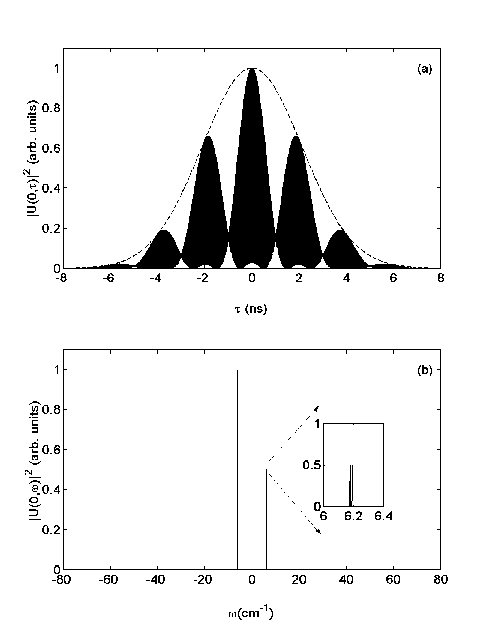
\includegraphics[width=5in]{nlsetime.pdf}
\end{center}
\renewcommand{\baselinestretch}{1}
\small\normalsize
\begin{quote}
\caption[Multimode pulse input toe NLSE]
{Multimode pulse input to the NLSE: (a) input pulse in time
domain and (b) input spectrum.}
\label{figA.1}
\end{quote}
\end{figure}
\renewcommand{\baselinestretch}{2}
\small\normalsize

The basic form of the initial complex wave envelope function is
%A.10
\begin {equation}
U(0,\tau) = exp \left( - {\tau^2 \over 2\tau_p^2} \right)
\left\{
\begin{array}{l}
exp\left( {i\Omega\tau \over 2} \right) + \\
exp\left( - {i\Omega\tau \over 2} \right)
\end{array}
\right\} ,
\end{equation}
where $\tau_p$ is the pulse width T$_p$ =5\,ns FWHM, normalized to the time scale
T$_0$, $\Omega$=366\,GHz is the frequency detuning between the two laser
sources normalized to a frequency scale $\Omega_0$ = 62.5\,MHz.  Figure A.1(a)
shows a plot of this pulse $|U(0,\tau)|^2$. The overall Gaussian envelope
has an FWHM of 5\,ns, the closely spaced dark lines are due to the 366\,GHz
($\sim$3\,ps) beating between the two input pump frequencies. The 2\,ns
modulations on the pulse are due to the 0.5\,GHz mode-structure in the
blue-shifted pump wave. Figure A.1(b) shows the input spectrum of this pulse
which consists of two highly monochromatic pump waves with a detuning of
$\Omega$=366\,GHz. The spectrum of the blue-shifted pump, upon magnification,
is seen to be composed of two very closely spaced peaks, with a separation of
$\Delta\nu$=0.5\,GHz. Hart {\it et al}.\ \cite{hart1} did not use pulsed
wave functions in their NLSE simulations as the size of the FFT required to do
so made it computationally prohibitive at that time. The size of the FFT was
chosen such that it would accommodate a time span of 16\,ns in order to go
sufficiently far into the wings on the Gaussian pulse; and a frequency span of
16\,THz in order to accommodate all the sidebands generated and prevent
spurious effects due to the reflection boundary conditions implicit in the
SSFM algorithm. These considerations dictated the size of the FFT to be
$\geq$(16 THz)$\cdot$(16 ns) = 256000. The nearest power of 2 is
2$^{18} = 262144$, which has been used throughout the present work. The
incorporation of the pulsed nature of the light was found to be necessary in
explaining the dynamics. From the perspective of the coupled amplitude
equations used by Hart {\it et al}.\ \cite{hart1}, the present model is equivalent
to a coupled-ODE model with $2^{18}$ coupled ODEs.

%Figure A.2
\begin{figure}
\begin{center}
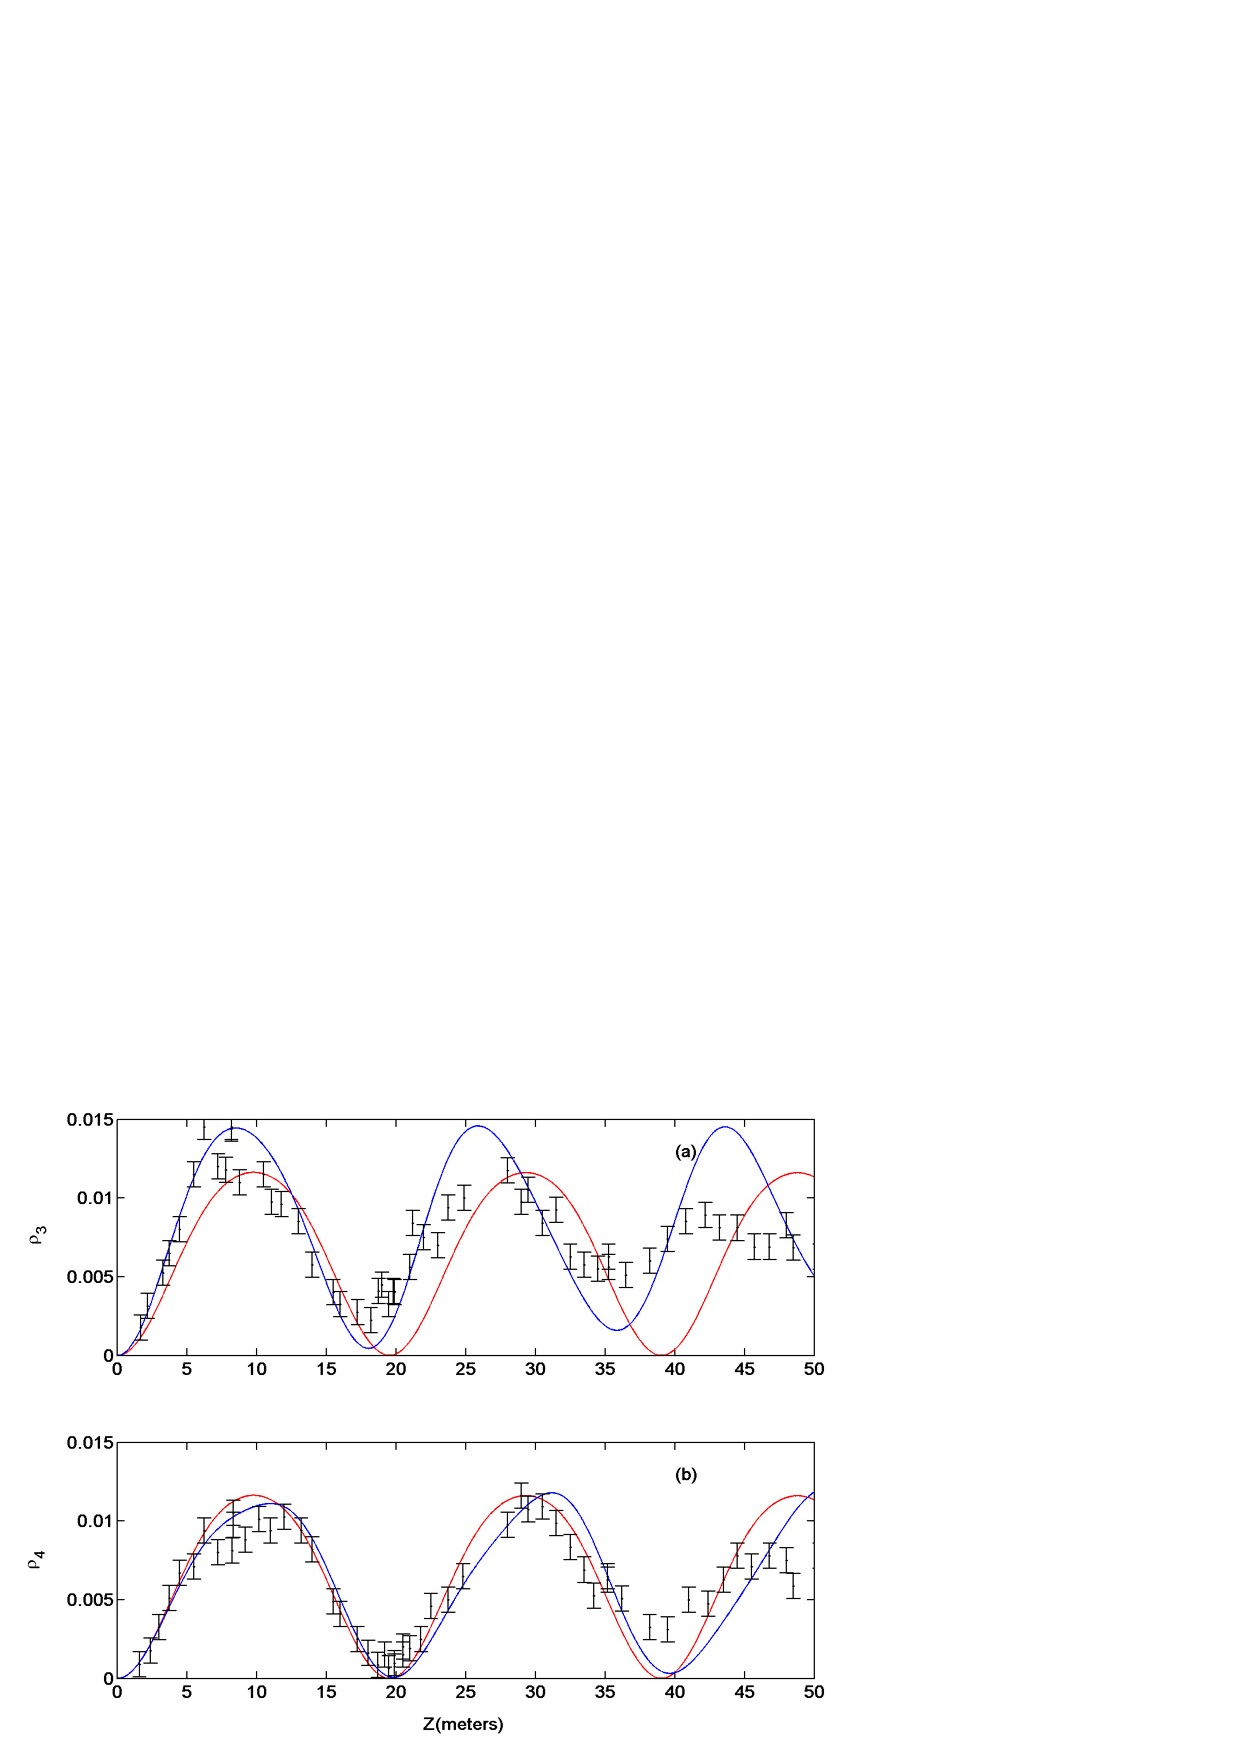
\includegraphics[width=5in]{modestruc21ornot.pdf}
\end{center}
\renewcommand{\baselinestretch}{1}
\small\normalsize
\begin{quote}
\caption[Short caption for Figure A.2.]
{Effects of inclusion of the multimode nature ($\Delta\nu = 0.5$\,GHz) of the blue-shifted input pump laser on the 1st order sideband evolution as a function of fiber length for P$_0 = 2.1$\,W. Dashed curves represent simulations without the multimode nature and solid curves represent simulations with the multimode nature. $\Omega = 366$\,GHz, $\gamma = 0.019$\,W$^{-1}$\,m$^{-1}$, and $\beta^{(2)} = 55$\,ps$^2$/km (a) power in the blue-shifted sideband, (b) power in the red-shifted sideband.}
\label{figA.2}
\end{quote}
\end{figure}
\renewcommand{\baselinestretch}{2}
\small\normalsize

%Figure A.3
\begin{figure}
\begin{center}
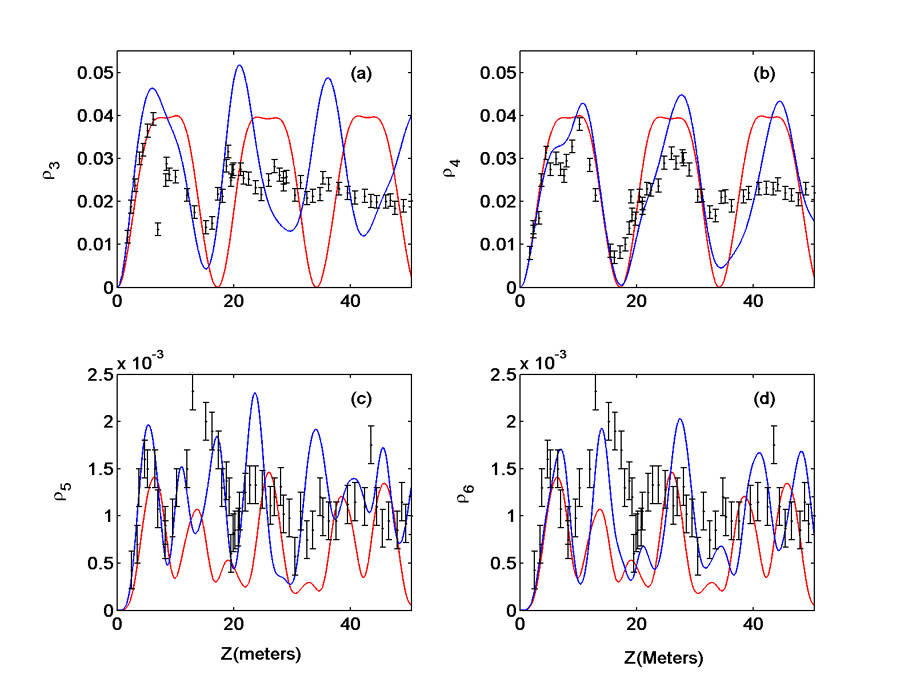
\includegraphics[width=5in]{modestruc55ornot.pdf}
\end{center}
\renewcommand{\baselinestretch}{1}
\small\normalsize
\begin{quote}
\caption[Effects of inclusion of the multimode nature]
{Effects of inclusion of the multimode nature ($\Delta\nu = 0.5$\,GHz) of the blue-shifted input pump laser on the 1st order sideband evolution as a function of fiber length for P$_0 = 5.5$\,W. Dashed curves represent simulations without the multimode nature and solid curves represent simulations with the multimode nature. $\Omega = 366$\,GHz, $\gamma = 0.019$\,W$^{-1}$\,m$^{-1}$, and $\beta^{(2)} = 55$\,ps$^2$/km (a) power in the first-order blue-shifted sideband, (b) power in the first-order red-shifted sideband, (c) power in the second-order blue-shifted sideband, (d) power in the second-order red-shifted sideband.}
\label{figA.3}
\end{quote}
\end{figure}
\renewcommand{\baselinestretch}{2}
\small\normalsize

%Figure A.4
\begin{figure}
\begin{center}
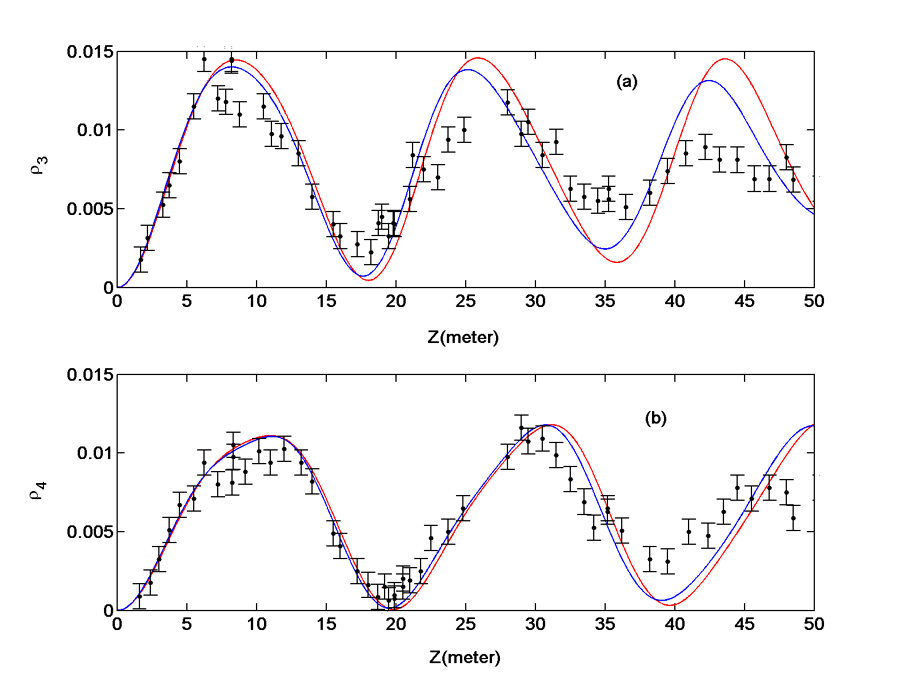
\includegraphics[width=5in]{nlsez21cwpulse.pdf}
\end{center}
\renewcommand{\baselinestretch}{1}
\small\normalsize
\begin{quote}
\caption[Effects of inclusion of the pulsed nature]
{Effects of inclusion of the pulsed nature (5\,ns FWHM) of the input pump laser light on the first-order sideband evolution as a function of fiber length for P$_0 = 2.1$\,W. Dashed curves represent cw simulations and solid curves represent pulsed simulations. $\Omega = 366$\,GHz, $\Delta\nu = 0.5$, $\gamma = 0.019$\,W$^{-1}$m$^{-1}$, and $\beta^{(2)} = 55$\,ps$^2$/,km (a) power in the blue-shifted sideband, (b) power in the red-shifted sideband.}
\label{figA.4}
\end{quote}
\end{figure}
\renewcommand{\baselinestretch}{1}
\small\normalsize

%Figure A.5
\begin{figure}
\begin{center}
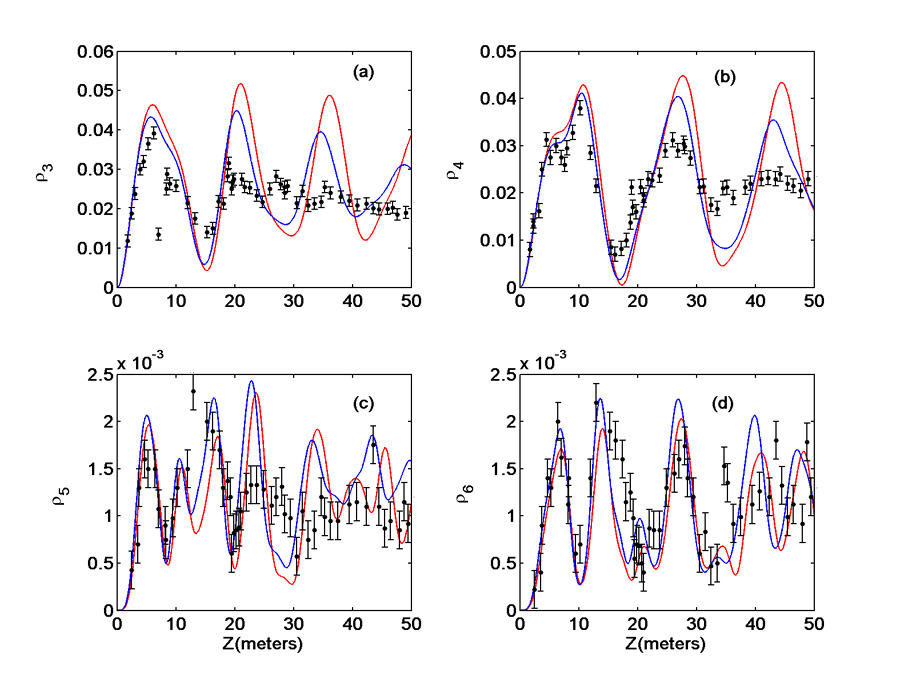
\includegraphics[width=5in]{nlsez55cwpulse.pdf}
\end{center}
\renewcommand{\baselinestretch}{1}
\small\normalsize
\begin{quote}
\caption
[Other effects of inclusion of the pulsed nature]
{Effects of inclusion of the pulsed nature (5\,ns FWHM) of the input pump laser on the first- and second-order sideband evolution as a function of fiber length for P$_0 = 5.5$\,W. Dashed curves represent cw simulations and solid curves represent pulsed simulations. $\Omega = 366$\,GHz, $\Delta\nu = 0.5$, $\gamma = 0.019$\,W$^{-1}$m$^{-1}$, and $\beta^{(2)} = 55$\,ps$^2$/,km (a) power in the first-order blue-shifted sideband, (b) power in the first-order red-shifted sideband, (c) power in the second-order blue-shifted sideband, (d) power in the second-order red-shifted sideband.}
\label{figA.5}
\end{quote}
\end{figure}
\renewcommand{\baselinestretch}{2}
\small\normalsize

Upon incorporation of the multimode nature of the blue input pump laser source
and the stochastic fluctuations in the initial power in the lasers, the
initial wave function takes the form
%A.11
\begin{equation}
U(0,\tau) = exp\left( - {\tau^2 \over 2\tau_p^2} \right)
\left\{
\begin{array}{l}
\sqrt{{1 + \delta\rho_1 \over 2}}
\left[ \begin{array}{l}
exp \left( {i(\Omega+\Delta\nu)\tau \over 2} \right) + \\
exp \left( {i(\Omega-\Delta\nu)\tau \over 2} \right)
\end{array} \right]\\
+ \sqrt{1 + \delta\rho_2} exp\left( - {i\Omega\tau \over 2} \right)
\end{array}
\right\}.
\end{equation}

\

\noindent $\Delta\nu = 0.5$\,GHz is the frequency separation between the two longitudinal
modes in the blue-shifted pump. $\delta\rho_1$ and $\delta\rho_2$ are
Gaussian random deviates (generated using the Box-Muller algorithm
\cite{boxmuller}) that represent the initial power fluctuations in each of the
pump laser sources. Their standard deviations were taken to be,
$\sigma_{\rho_1} = 0.2$, $\sigma_{\rho_2} = 0.11$ for simulations from 0\,m to
20\,m, $\sigma_{\rho_1} = 0.12$, $\sigma_{\rho_2} = 0.05$ for simulations from
20\,m to 50\,m along the length of the fiber. This is exactly the same
prescription used by Hart {\it et al}.\ \cite{hart1} in their simulations and is
dictated by their experimental measurements of the fluctuations in the pump
laser intensities.

At this point it is worth noting the effects of the inclusion of two attributes of
the input laser light, namely, the multimode nature of the blue-shifted pump, and
the pulsed nature of the input light (assumed to be cw in the simulations reported by
Hart {\it et al}.\ \cite{hart1}).

Figure A.2 shows a comparison between simulations with (solid curves) and without (dashed curves) the multimode nature for an input pump power of 2.1 Watts. The simulations with the mode structure show the asymmetry between the blue- and red-shifted sideband evolution, in particular, the difference in spatial wavelength between the two, and a non-return to zero nature of the evolution, as observed in the experimental data (black dots with error bars). These features are absent in the simulations without mode-structure. $\rho_3$ and $\rho_4$ stands for the first order blue- and red-shifted sidebands respectively.  Figure 2.3 shows the corresponding comparison for the case of 5.5 Watts of input pump power.  Here, too, the simulations incorporating the multimode nature of the blue-shifted pump (solid curves) are seen to be an improvement over those not incorporating it (dashed curves). A feature of the experimental data (black dots with errorbars) is that for the $\rho_3$ sideband, the initial part of the evolution involves a peak followed by a shoulder, while for the $\rho_4$ sideband, the initial part of the evolution involves a shoulder followed by a peak. This feature, too, is seen to occur as a result of the inclusion of the multimode nature of the blue-shifted pump.

The effect of inclusion of the pulsed nature of the input beam is seen in Fig.\ A.4 (for the 2.1 Watt case) and Fig.\ A.5 (for the 5.5 Watt case). The solid dashes represent simulations for a cw input beam and the solid curves represent those for a pulsed input beam. The incorporation of the pulsed nature clearly results in damping of the sideband trajectories which are seen to come closer to the experimental data \cite{hart1} (black dots with error bars).

Use of the FFT algorithm makes evaluation relatively fast compared to other
finite-difference schemes. The computational error is $O(\Delta z^2)$, thus
the solution converges with decreasing spatial step-size $\Delta z$.

The simulations were tested for the conservation of total power along the
fiber length (by setting the loss $\alpha$ to zero) and for the conservation
of asymmetry \cite{thompson1,hart1} given by
%A.12
\begin{equation}
C(Z) = \sum_{i=1}^{\infty}(2i-1)[\rho_{2i-1}(Z)-\rho_{2i}(Z)] .
\end{equation}

A clearer picture of the evolution of the sidebands is obtained by plotting both the
power in the sidebands and their standard deviations as a function of length along the fiber. Figures A.6(a) and A.6(b) show a comparison between simulation and experiment of the evolution
of the first-order blue-shifted ($\rho_3$) and red-shifted ($\rho_4$) sidebands,
respectively, for an input power of 2.1 W. The dashed curves represent NLSE simulations
which include the stochastic nature of the input powers of the pump lasers but exclude
the stochastic phase fluctuations added along the length of the fiber, an attribute
which is included in the simulations represented by the solid curves. The black dots
with error bars represent the experimental data. The measured sideband
power, normalized to the total power in the fiber, is periodic in length but
appears to be damping to a constant value. The measured data also show a clear
difference between the spatial wavelengths of oscillation of the blue-shifted ($\rho_3$) and red-shifted ($\rho_4$) sidebands trajectories, respectively. Both these features are captured well by both the simulations. Figures A.6(c) and A.6(d) compare experimental and simulated
measures of the evolution of the standard deviation in the sideband power
along the fiber length. It is clearly observed that simulations with phase noise
added to the light field along the length of the fiber (solid curves) are closer to the
experimental data as compared to those that exclude this feature (dashed curves). This indicates
the instrumental nature of the phase fluctuations in explaining key features of the dynamics.

%Figure A.6
\begin{figure}
\begin{center}
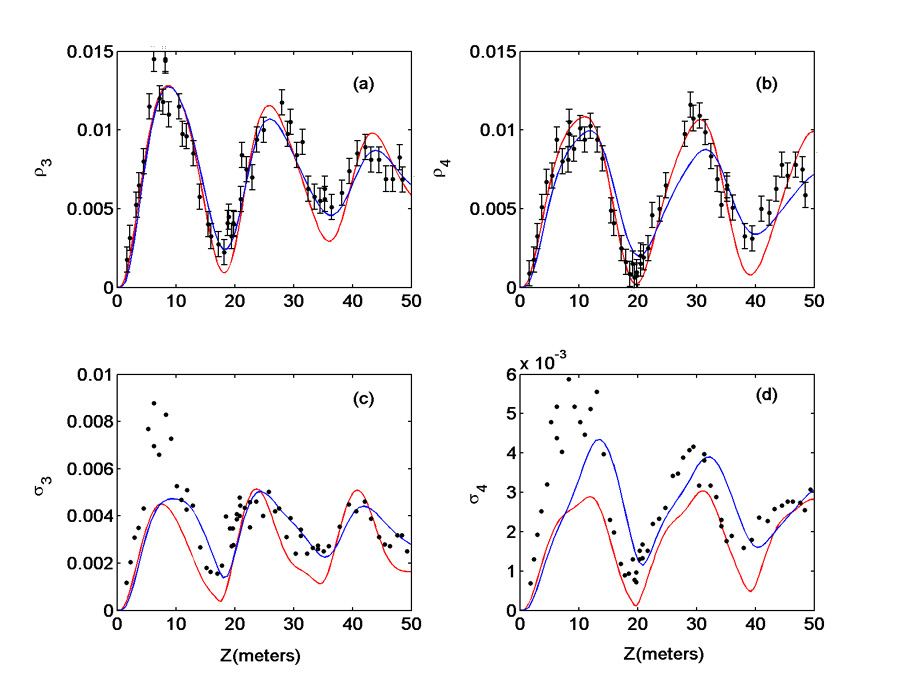
\includegraphics[width=5in]{nlsez21phaseornot.pdf}
\end{center}
\renewcommand{\baselinestretch}{1}
\small\normalsize
\begin{quote}
\caption
[Comparison between experiments measurements]
{Comparison between the experimental measurements \cite{hart1}(black), the random initial condition NLSE model excluding phase noise (dashed curves) and the stochastic phase noise NLSE model (solid curves) showing the first-order sideband evolution as a function of fiber length for P$_{0} = 2.1$\,W, $\Omega = 366$\,GHz, $\Delta\nu = 0.5$\,GHz,$\gamma = 0.019$\,W$^{-1}$m$^{-1}$, and $\beta^{(2)} = 55$ps$^2$/km: dynamical evolution of the: (a) power in the blue-shifted sideband, (b) power in the red-shifted sideband, (c) fluctuations in the blue-shifted sideband, (d) fluctuations in the red-shifted sideband.}
\label{figA.6}
\end{quote}
\end{figure}
\renewcommand{\baselinestretch}{2}
\small\normalsize

The apparent damping of the periodic sideband trajectory is seen more
dramatically in Figs.\ A.7(a) and A.7(b), which show the evolution of the
first-order sideband power along the fiber for an input power of 5.5\,W.
The two first-order sidebands evolve differently. They appear to
damp to a constant value at a faster rate than for the case with an input pump
power of 2.1\,W. Here again, NLSE simulations that incorporate phase noise along the length
of the fiber (solid curves) are much more successful in accurately capturing the dynamical features of the system than NLSE simulations that do not take this feature into account (dashed curves).  Figures A.7(c) and A.7(d) show a comparison between the simulated and measured standard deviations. Comparisons for the second-order blue-shifted ($\rho_5$) and red-shifted ($\rho_6$) sidebands, respectively, are shown in Figs.\ A.7(e) and A.7(f).


%Figure A.7
\begin{figure}
\begin{center}
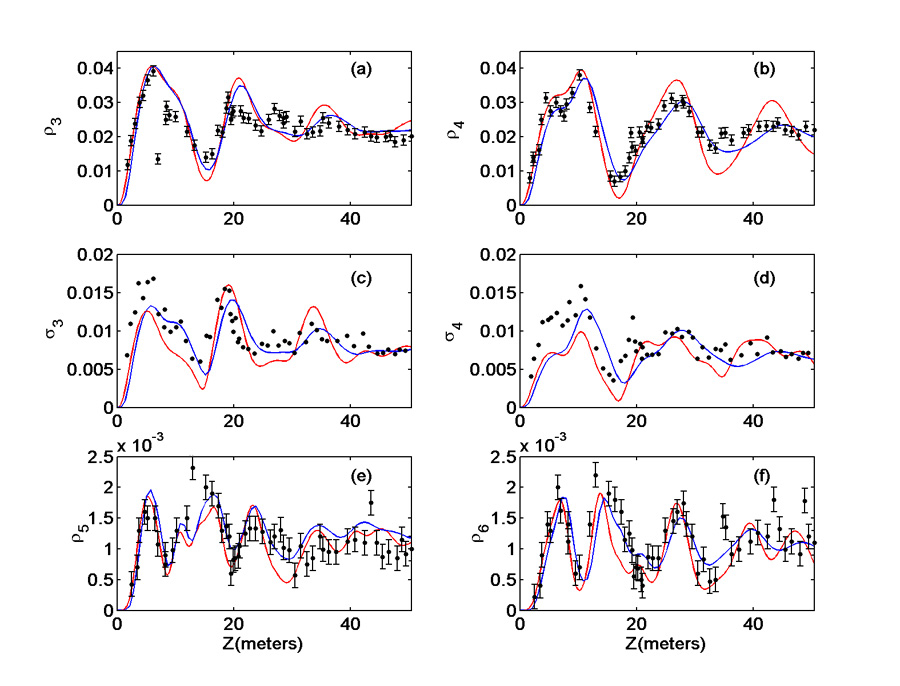
\includegraphics[width=5in]{nlsez55phaseornot.pdf}
\end{center}
\renewcommand{\baselinestretch}{1}
\small\normalsize
\begin{quote}
\caption
[This figure caption is indented and single-spaced]
{This figure caption is indented and single-spaced.  Comparison between the experimental measurements \cite{hart1} (black), the random initial condition NLSE model excluding phase noise (dashed curves) and the stochastic phase noise NLSE model (solid curves) showing the first- and second-order sideband evolution as a function of fiber length for P$_{0} = 5.5$\,W, $\Omega = 366$\,GHz, $\Delta\nu = 0.5$\,GHz, $\gamma = 0.019$\,W$^{-1}$m$^{-1}$, and $\beta^{(2)} = 55$\,ps$^2$/km: dynamical evolution of the: (a) power in the first-order blue-shifted sideband, (b) power in the first-order red-shifted sideband, (c) fluctuations in the first-order blue-shifted sideband, (d) fluctuations in the first-order red-shifted sideband, (e) power in the second-order blue-shifted sideband, (f) power in the second-order red-shifted sideband.}
\label{figA.7}
\end{quote}
\end{figure}
\renewcommand{\baselinestretch}{2}
\small\normalsize

The observed dynamical evolution of the sidebands is found to depend
sensitively on the strength of the stochastic phase fluctuations. Yet, best
agreement with the experimental results of Hart {\it et al}.\ \cite{hart1} is
achieved with exactly the same noise strength $\sigma^2_\phi$ as used in
their truncated ODE model, namely, $\sigma^2_\phi = 0.0067$\,m$^{-1}$. They
report that including phase noise in their FWM calculations resulted in a
spurious linear drift in the trajectories for the sideband power with length.
To remove this artifact of the computations, they added a linear loss to their
coupled ODEs. They set the loss coefficient $\alpha = 0.0046$\,m$^{-1}$ by
finding the value that removed this increasing slope. We have observed exactly
the same secular growth phenomenon for a wide range of the noise strength
$\sigma^2_\phi$ and have arrived at an empirical prescription for $\alpha$
namely, $\alpha\sim\sigma^2_\phi$, where $\sigma^2_\phi$ is the
variance of the added phase noise. This indicates the general nature of
dynamics resulting from the addition of stochastic, $\delta$-correlated phase
fluctuations to systems governed by nonlinear partial differential equations
\cite{risken}.

It is remarkable that the strength of the phase noise required is the same in
both the 2.1\,W and the 5.5\,W cases. Further, it is worth noting that exactly
the same noise strength was used by Hart {\it et al}.\ \cite{hart1}, the difference
being that they introduced phase noise only in the pump frequencies, whereas
we have introduced it in all the Fourier modes ($\sim2^{18}$). As a
confirmation of this result, they also performed experiments and numerical
simulations examining the sideband power dependence on the input power at a
fixed length of 50.4\,m of the same fiber. We have repeated these simulations
with the stochastic NLSE model and the results are shown in Figs.\ 2.8(a)
(blue-shifted sideband) and 2.8(b) (red-shifted sideband). The experimental
measurements of the sideband powers are represented by filled squares and the
results of numerical simulations are represented by triangles (without phase
noise) and by circles (with phase noise). The simulations are seen to follow
the general trend seen in the experiments. As the pump power is increased, the
triangles (without phase noise) start to disagree with experiment, whereas the
circles (with phase noise) are much closer to experiment. The phase noise
strength used in these simulations was exactly the same as that used in the
simulations depicted in Figs.\ A.6 and A.7. The agreement between the phase noise
simulations and the experimental data was (once again) highly sensitive to the
noise strength. Since this experiment (unlike those shown in Figs.\ A.2 - A.7)
is non-destructive, it can be used to deduce the strength of phase noise
processes in a given optical fiber. It will be shown in Sec.\ 2.4 that a
likely cause of the phase noise is fluctuation in the linear refractive index
of the fiber. The noise strength deduced from the present computational study
corresponds to a refractive index inhomogeneity of
$\langle \Delta n^{2} \rangle \sim 10^{-16}$.

%Figure A.8
\begin{figure}
\hspace{1.25in}
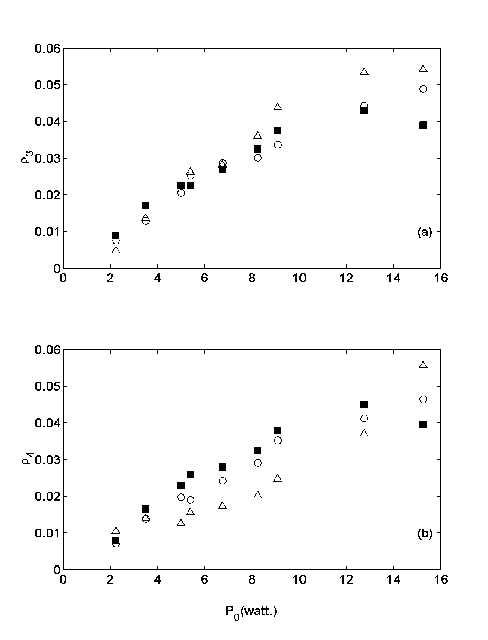
\includegraphics[width=5in]{nlsefinal.pdf}
\renewcommand{\baselinestretch}{1}
\small\normalsize
\begin{quote}
\caption
[Comparison between the experiments measurements (filled squares)]
{Comparison between the experimental measurements (filled squares), simulations without stochastic phase fluctuations (open triangles) and with stochastic phase fluctuations (open circles) of the first-order sideband power versus pump input power for L=50.39\,m, and $\Omega = 366$\,GHz: power in the (a) blue-shifted sideband and (b) red-shifted sideband.}
\label{figA.8}
\end{quote}
\end{figure}
\renewcommand{\baselinestretch}{2}
\small\normalsize

%Figure A.9
\begin{figure}
\begin{center}
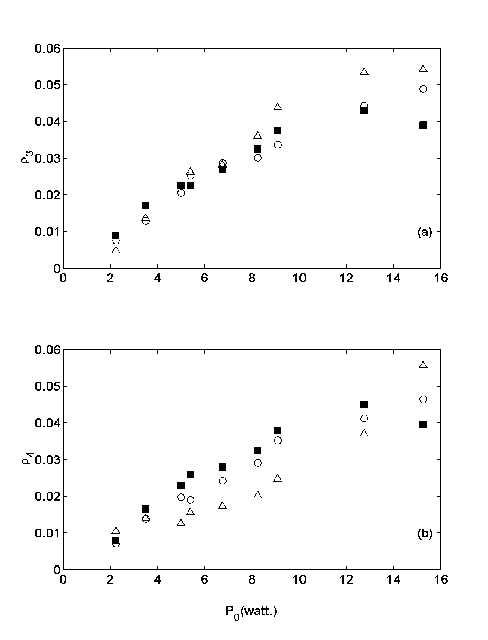
\includegraphics[width=5in]{nlsefinal.pdf}
\end{center}
\renewcommand{\baselinestretch}{1}
\small\normalsize
\begin{quote}
\caption
[Evolution of the FWM spectrum]
{Evolution of the FWM spectrum along the fiber (a) P=2.1\,W, experiment, (b) P=5.5\,W, experiment, (c) P=2.1\,W, stochastic-NLSE model, (d) P=5.5\,W, stochastic-NLSE model.}
\label{figA.9}
\end{quote}
\end{figure}
\renewcommand{\baselinestretch}{2}
\small\normalsize

Till now the comparisons between our simulations of the full NLSE and the
truncated ODE model give basically the same results, although with much better
agreement with experiment. However, the full NLSE can also provide a detailed
comparison with the experimental spectra. This was not available from the
truncated ODE model. The simulations reported in this work were carried out
with a very high frequency and time resolution in order to incorporate the
fact that the input light was not cw, but was composed of $\sim$ 5\,ns long
pulses; and that the number of sidebands generated required the frequency
spread of the FFT to be $\sim$ 16\,THz, while resolving a longitudinal
mode-structure of $\Delta\nu$ $\sim 0.5$\,GHz. The spectral resolution used was
$\sim$ 0.05\,GHz, whereas the spectrometer used to observe the spectra had a
resolution 1000 times larger ($\sim$ 50\,GHz). To account for this difference,
the simulated spectra were first convolved with a Gaussian of unit peak and
62\,GHz FWHM, before they were compared with the observed spectra.

Figures A.9(a) and A.9(b) show three-dimensional plots of the average experimental
FWM output spectrum along the length of the fiber for input pump powers of 2.1\,W and 5.5\,W,
 respectively (courtesy Hart {\it et al}.\ \cite{hart1}). The vertical
axis represents the intensity, normalized to the peak power in one of the
input pumps, plotted on a logarithmic scale. The pump frequencies are centered
on $+/-\Omega/2$ and the fiber length is increasing into the page. Figures
9(c) and 9(d) show the corresponding comparisons based on simulations using
the stochastic-NLSE model. The basic features of the spectral evolution are
captured by the simulations.

%Figure  A.10
\begin{figure}
\begin{center}
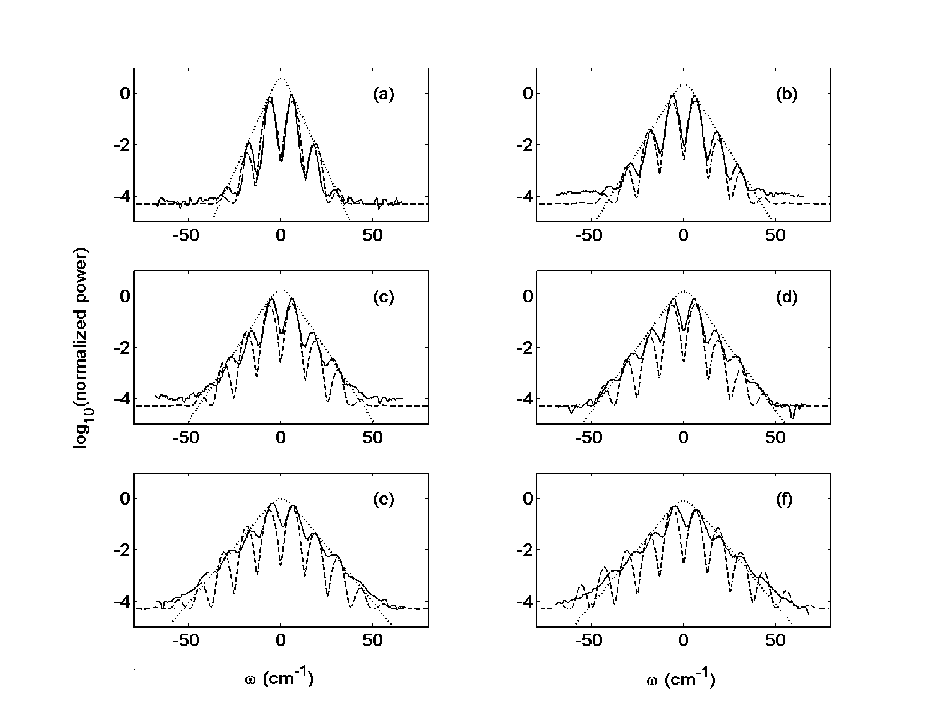
\includegraphics[width=5in]{nlsespec.eps}
\end{center}
\renewcommand{\baselinestretch}{1}
\small\normalsize
\begin{quote}
\caption
[Experimental FWM output spectrum]
{Experimental FWM output spectrum (solid line), convolved spectra from simulations of the stochastic NLSE model (dashed line), and hyperbolic secant envelope fit (dotted line) for pump input powers P$_0$ of (a) 2.1\,W, (b) 5.5\,W, (c) 6.7\,W, (d) 8.3\,W, (e) 12.7\,W, (f) 17.4\,W, fiber length L$= 50.39$\,m, $\Omega = 366$\,GHz, $\Delta\nu = 0.5$\,GHz, $\gamma = 0.019$\,W$^{-1}$m$^{-1}$, and $\beta^{(2)} = 55$\,ps$^2$/km.}
\label{figA.10}
\end{quote}
\end{figure}
\renewcommand{\baselinestretch}{2}
\small\normalsize

Hart {\it et al}.\ \cite{hart1} also documented the experimentally observed FWM
output spectra for a fixed fiber length of 50.39 meters for 6 different input
pump powers. They state the coefficients A and B of the hyperbolic secant
envelopes that best fit the output spectra which are given by
%A.13
\begin{equation}
f(\omega) = Asech(B\omega) ,
\end{equation}
where A and B are the experimental fit parameters.

The hyperbolic secant parameters A and B, that best fit the simulated spectra
are exactly the same as those that best fit the experimental spectra
\cite{hart1} for all the 6 cases of input power considered. Figure 2.10 shows an
overlap of the simulated spectra (dashed line), with the experimental spectra
(solid line) and the experimental hyperbolic secant envelope (dotted line) for
6 different pump powers, namely, (a) 2.1\,W, (b) 5.5\,W, (c) 6.7\,W, (d) 8.3\,W, (e)
12.7\,W, (f) 17.4\,W. The hyperbolic secant parameters for each of these pump
powers are (a) A=3.85 and B=0.36, (b) A=2.26 and B=0.27, (c) A=1.81, B=0.25,
(d) A=1.56 and B=0.23, (e) A=0.98,B=0.20, and (f) A=0.81 and B=0.20. The exact
shapes of the simulated spectra match very well with the experimental spectra
for low input pump powers (2.1\,W and 5.5\,W), but tend to lack the "filled-in"
character of the experimental spectra at higher powers (6.7\,W, 8.3\,W, 12.7\,W and
17.4\,W).

\section{Discussion}

Hart {\it et al}.\ \cite{hart1} postulated that strong candidates for the possible
physical sources of the phase fluctuations are stimulated Brillouin
scattering, stimulated Raman scattering and fiber medium inhomogeneities.
Brillouin scattering was eliminated as a source, since a backward propagating
wave, which is a signature of Brillouin scattering in optical fibers, was not
observed in the experiments. We have  modeled stimulated Raman scattering
\cite{Agrawal8, headley} for our system and have found no evidence to
support the hypothesis that it could be a possible source of the stochastic phase
fluctuations for fiber lengths up to 50 meters and pump power levels up to 5.5 Watts.
A more detailed discussion of the Raman scattering simulations performed is given in Chap.\ 3.
Apart from these, quantum phase fluctuations are another well
known, though extremely weak, source of phase noise in optical fibers
\cite{Agrawal2,perlmutter1}.

Fiber medium inhomogeneities were identified as the major cause of the
stochastic phase fluctuations. These inhomogeneities can manifest themselves
through spatial and/or temporal fluctuations in the fiber parameters, namely,
the linear refractive index $n_0$, the group velocity $v_g$, the group
velocity dispersion $\beta^{(2)}$ and the nonlinearity
$\gamma$ \cite{abdullaev}. Of these, the fluctuation in the linear refractive
index was found to be the only source of phase fluctuation that had a
significant effect on the dynamics. A relationship between the level of
refractive index fluctuations and the  corresponding level of phase
fluctuations has been arrived at. It is found that refractive index
fluctuations as small as $\sigma_n^2 \sim 10^{-17}$\,m$^{-1}$ can cause the
desired phase fluctuations. Possible sources of these refractive index
fluctuations are discussed below.

Consider the modified nonlinear Schr\"odinger equation (NLSE) which is
stated below, with the linear multiplicative noise term represented in terms of
spatial and temporal fluctuations in the refractive index of the fiber.
%A.14
\begin{equation}
{\partial U \over \partial z} + {i\beta^{(2)} \over 2T_0^2} {\partial^2U \over \partial\tau^2} + {\alpha U \over 2} + ik_0 \delta n(z,\tau)U - i\gamma P_{0}|U|^2 U = 0 ,
\end{equation}
where $\delta n(z,\tau)$ is the spatial and temporal variation of the refractive
index along the fiber. It can be caused by temperature and density
fluctuations in the fiber \cite{glenn}.

The thermodynamic estimate for $\Delta n$ is given by \cite{glenn}
%A.15
\begin{equation}
\langle \Delta n^{2} \rangle = {-kT\rho^2 \over V^2}
\left( {\partial V \over \partial P} \right)_{T}
\left( {\partial n \over \partial \rho} \right)_{T}^{2}
 + {kT^2 \over \rho VC_v} \left( {\partial n \over \partial T} \right)_{\rho}^2 .
\end{equation}

This gives the mean-square index fluctuation in terms of the properties of
the material. It can be rewritten as
%A.16
\begin{equation}
\langle \Delta n^{2} \rangle = {V_{\rho}+V_T \over V} = \langle \Delta n^{2} \rangle_{\rho}+\langle \Delta n^{2} \rangle_{T} .
\end{equation}

For a fiber of length z=1\,m and radius r=2.82\,$\mu$m
(Volume V=2.5 $\times 10^{-12}$\,m$^3$), these have been calculated to be
%A.17
\begin{eqnarray}
\langle \Delta n^2 \rangle_{\rho} \sim 10^{-21} & \equiv & \langle \Delta \rho^2 \rangle \sim 10^{-14}
{kg^2 \over m^6}, \nonumber \\
\langle \Delta n^2 \rangle_T \sim 10^{-23} & \equiv & \langle \Delta T^2 \rangle \sim 10^{-12}~{^\circ}C^2 .
\end{eqnarray}

It should be noted that $\langle \Delta n^2 \rangle \propto (1/z) \Rightarrow \delta n \propto  (1 / \sqrt{z})$. The corresponding phase fluctuation that this would lead to in the NLSE is given by $\delta \phi=k_{0} \delta n z \propto \sqrt {z}$, which is equivalent to the prescription for incorporating phase fluctuations into the stochastic NLSE model described in Sec.\ 2.3, namely,  $\langle \Delta \phi^2 \rangle = 6.7 \times 10^{-3}z$. Hart {\it et al}.\ \cite{hart1} used the same prescription and the same noise strength in their truncated-ODE model. From this we can estimate the level of refractive index fluctuation that corresponds to the noise strength used in the simulations described in Sec.\ 2.3
%A.18
\begin{eqnarray}
\langle \Delta n^2 \rangle = {6.7 \times 10^{-3} \over k_0^2} = 6.78 \times 10^{-17} \nonumber\\
\equiv \langle \Delta T^{2} \rangle \sim 10^{-6}~{^\circ}C^2 \equiv \Delta T \sim 10^{-3}~{^\circ}C
\end{eqnarray}

The temperature coefficient of the refractive index of silica \cite{glenn},
$(\partial n / \partial T)_{\rho} \sim 10^{-5} ~{^\circ}C^{-1}$. Thus even small spatio-temporal temperature fluctuations of $\sim 10^{-3} ~{^\circ}C$ are enough to cause the inferred level of refractive index fluctuations.

The refractive index fluctuations could also be due to inhomogeneities in the
density of the fiber material, frozen in at the time of manufacture of the
fiber. The simulations were averaged over $\sim$ 600 iterations to get a good
estimate of the power fluctuations in the sidebands. Initially, simulations
were performed with a different phase noise distribution for each iteration.
Later, a particular (arbitrary) phase noise distribution was selected and
frozen for all the iterations.
This did not reduce the level of damping observed in the sideband trajectories
provided that the strength of the phase noise was kept the same, thus
indicating that density fluctuations induced during fiber manufacture could be
a possible source. The phase noise was modeled as $\delta$-correlated in
both space and time. A more realistic approach would be to use correlated
noise. Numerical methods to incorporate linear multiplicative correlated noise
into the NLSE have been developed by M.J. Werner {\it et al}.\ \cite{werner2}.

\section{Conclusions}

The role of stochasticity in the dynamical evolution of four-wave-mixing
processes in an optical fiber has been investigated. This research consisted
of theoretical and numerical computations. It focuses on tracing the evolution
of the sidebands, generated through FWM, along a length of optical fiber.
Detailed comparisons were made with the experimental results of
Hart {\it et al}.\ \cite{hart1} and the agreement was excellent. The present work
uses numerical techniques that have much higher resolution and better
efficiency, and it presents a theoretical basis for the role of the
stochasticity in the dynamics. The system is known to be governed by the
nonlinear Schr\"odinger equation (NLSE) to a very good
approximation \cite{Agrawal2}.

A powerful technique that can be used for simulations of the stochastic NLSE
is the Split-step Fourier Method (SSFM) \cite{Agrawal2}. An algorithm for the
direct implementation of stochastic processes along the length of the fiber in
the SSFM has been developed. The advantages of this approach with respect to
the coupled-ODE approach are that we can carry out simulations with much
higher frequency and time resolution without sacrificing computational
efficiency.

The physical sources of these stochastic phase fluctuations are investigated
quantitatively and are identified to be due to fluctuations in the linear
refractive index of the fiber. Strong candidates for the causes of these
refractive index fluctuations are temperature fluctuations in the fiber medium
caused by the fluctuating temperature of the fiber environment, density
fluctuations in the fiber medium frozen into the fiber during manufacture, and
intrinsic thermodynamic fluctuations in the temperature and density of the
fiber.

The experiments performed by Hart {\it et al}.\ \cite{hart1} can be used to
determine the level of these refractive index fluctuations in commercial
fibers. Results described in Figs.\ 2 and 3 represent a destructive
experiment that measures the sideband evolution with fiber length for a fixed
input pump power, necessarily requiring the fiber to be cut repeatedly. The
level of refractive index fluctuations can be used as a parameter in the
simulations to best fit the experimental results. Alternatively, Fig.\ 4
represents a non-destructive experiment that measures the sideband evolution
with input pump power for a fixed fiber length. These experiments are found to
be effective for estimating the refractive index fluctuations, as the dynamics
is observed to be sensitively dependent on the strength of the phase
fluctuations.


%\renewcommand{\baselinestretch}{1}
%\small\normalsize
%\begin{thebibliography}{99}
\setlength{\parskip}{1em}

\bibitem{Agrawal1} G.P. Agrawal, {\em Nonlinear Fiber Optics} (Academic
Press, San Diego, CA, 2001), Chap. 1.
\bibitem{Bloembergen} N. Bloembergen, {\em Nonlinear Optics} (Benjamin,
Reading, MA, 1977).
\bibitem{Shen} Y.R. Shen, {\em Principles of Nonlinear Optics} (Wiley, New
York, 1984).
\bibitem{Butcher} P.N. Butcher and D.N. Cotter, {\em The Elements of
Nonlinear Optics} (Cambridge University Press, Cambridge, UK, 1990).
\bibitem{Boyd} R.W. Boyd, {\em Nonlinear Optics} (Academic Press, San Diego,
CA, 1992).
\bibitem{Newell} A.C. Newell and J.V. Moloney {\em Nonlinear Optics (Advanced Topics in the Interdisciplinary Mathematical Sciences)} (Westview Press, Boulder, CO, April 1992). 
\bibitem{Marcuse} D. Marcuse,{\em Light Transmission Optics} (Van Nostrand
Reinhold, New York, 1982), Chaps. 8 and 12.
\bibitem{Agrawal2} G.P. Agrawal, {\em Nonlinear Fiber Optics} (Academic
Press, San Diego, CA, 2001), Chap. 2.
\bibitem{Diament} P. Diament, {\em Wave Transmission and Fiber Optics}
(Macmillan, New York, 1990).
\bibitem{Zakharov} V.E. Zakharov and A.Shabat, Sov. Phys. JETP 
\textbf{34}, 62 (1972)
\bibitem{Hardin} R.H. Hardin and F.D. Tappert, SIAM
Rev. Chronicle \textbf{15}, 423 (1973).
\bibitem{Fisher} R.A.Fisher and
W.K. Bischel, Appl. Phys. Lett. \textbf{23}, 661 (1973); J. Appl. Phys
\textbf{46}, 4921 (1975).
\bibitem{Cooley} J.W. Cooley and J.W. Tukey,
Math. Comput. \textbf{19}, 297 (1965).
\bibitem{Trebino} R. Trebino, D.J. Kane, "Using phase retrieval to measure
the intensity and phase of ultrashort pulses: frequency resolved optical gating," J. Opt. Soc. Am. B \textbf{10}, 1101 (1993). 
\bibitem{Kanejqe} D.J. Kane, R. Trebino, "Characterization of Arbitrary Femtosecond Pulses Using Frequency-Resolved Optical Gating," IEEE J. Quant. Elect. \textbf{29}, 571 (1993). 
\bibitem{Kaneoptlett} D.J. Kane, R. Trebino, "Single-shot measurement of the intensity and phase of an arbitrary ultrashort pulse  by using frequency-resolved optical gating," Opt. Lett. \textbf{10}, 1101 (1993).
\bibitem{OShealett}P. O'Shea, M. Kimmel, X. Gu, R. Trebino, "Highly simplified device for ultrashort-pulse measurement," Opt. Lett. \textbf{26}, 932 (2001).
\bibitem{Agrawal3} G.P. Agrawal, {\em Nonlinear Fiber Optics} (Academic
Press, San Diego, CA, 2001), Chap. 3.
\bibitem{Agrawal4} G.P. Agrawal, {\em Nonlinear Fiber Optics} (Academic
Press, San Diego, CA, 2001), Chap. 4.
\bibitem{Agrawal10} G.P. Agrawal, {\em Nonlinear Fiber Optics} (Academic
Press, San Diego, CA, 2001), Chap. 10.
\bibitem{Agrawal7} G.P. Agrawal, {\em Nonlinear Fiber Optics} (Academic
Press, San Diego, CA, 2001), Chap. 7.
\bibitem{Agrawal6} G.P. Agrawal, {\em Nonlinear Fiber Optics} (Academic
Press, San Diego, CA, 2001), Chap. 6.
\bibitem{Stolen} R.H. Stolen, E.P. Ippen, and A.R. Tynes,
Appl. Phys. Lett. \textbf{20}, 62 (1972). 
\bibitem{Ippen} E.P. Ippen and R.H. Stolen, Appl. Phys. Lett. \textbf{21}, 
539 (1972). 
\bibitem{Smith} R.G. Smith, Appl. Opt. \textbf{11}, 2489 (1972).
\bibitem{Agrawal9} G.P. Agrawal, {\em Nonlinear Fiber Optics} (Academic
Press, San Diego, CA, 2001), Chap. 9.
\bibitem{Agrawal8} G.P. Agrawal, {\em Nonlinear Fiber Optics} (Academic
Press, San Diego, CA, 2001), Chap. 8.
\bibitem{hart1} D.L. Hart, Arthur F. Judy, Rajarshi Roy and James W. Beletic, Phys. Rev. E \textbf{57}, 4757 (1998); D.L. Hart, Arthur F. Judy, T.A.B. Kennedy, Rajarshi Roy and K. Stoev, Phys. Rev. A \textbf{50}, 1807 (1994).   
\bibitem{ito} K. Ito, {\em Lectures on Stochastic Processes} (Tata Institute of Fundamental Research, Bombay, 1960).
\bibitem{stratanovich} R.L. Stratanovich, {\em Topics in the Theory of Random Noise}, Vols I. and II. (Gordon \& Breach, New York, 1963).
\bibitem{risken} H. Risken, {\em The Fokker-Planck Equation} (Springer-Verlag, Berlin, 1989).
\bibitem{werner2} M.J. Werner and P.D. Drummond, J. Comput. Phys. \textbf{132}, 312 (1997).
\bibitem{drummond1} P.D. Drummond and I.K. Mortimer, J. Comput. Phys. \textbf{93}, 144 (1991).
\bibitem{carter3} S.J. Carter, Phys. Rev. A. \textbf{51}, 3274 (1995).
\bibitem{thompson1} J.R. Thompson and Rajarshi Roy, Phys. Rev. A \textbf{43}, 4987 (1991).
\bibitem{boxmuller} W.H. Press, S.A. Teukolsky, W.T. Vetterling and B.P. Flannery, {\em Numerical Recipes in Fortran: The Art of Scientific Computing} (Cambridge University Press, Cambridge, 1992).
\bibitem{headley} C. Headley, G.P. Agrawal, IEEE J. Quantum Electron. \textbf{QE-31}, 2058 (1995), C. Headley, G.P. Agrawal J. Opt. Soc. Am. B. \textbf{13}, 2170 (1995).
\bibitem{perlmutter1} S.H. Perlmutter, M.D. Levenson, R.M. Shelby and
M.B. Weisman, Phys. Rev. Lett. \textbf{61} 1388, 1988.
\bibitem{abdullaev} F. Kh. Abdullaev, J.H. Hensen, S. Bischoff and M.P. Sorensen, J. Opt. Soc. Am. B. \textbf{15}, 2424 (1998); F. Kh. Abdullaev, J.G. Caputo, and Nikos Flytzanis, Phys. Rev E. \textbf{50}, 1552 (1994).
\bibitem{glenn} William H. Glenn, IEEE J. Quantum Electron. \textbf{QE-25}, 1218 (1989).
\bibitem{Trebinobook} R. Trebino. {\em Frequency-Resolved Optical Gating: The Measurement of Ultrashort Laser Pulses} (Kluwer Academic 2002).
\bibitem{Agrawal} G.P. Agrawal {\em Nonlinear Fiber Optics} (Academic,
San Diego, 2001).
\bibitem{Dudley} J.M. Dudley, X. Gu, L. Xu, M. Kimmel, E. Zeek, P. O'Shea, R. Trebino, S. Coen, R.S. Windeler, "Cross-correlation frequency resolved optical gating analysis of broadband continuum generation in photonic crystal fiber: simulations and experiments," Opt. Express \textbf{10}, 1215 (2002).
\bibitem{Liu1} Q.D. Liu, J.T. Chen, Q.Z. Wang, P.P. Ho, and R.R. Alfano, "Single pulse degenerate-cross-phase modulation in a single-mode optical fiber," Opt. Lett. \textbf{20}, 542 (1995).
\bibitem{Sylvestre} T. Sylvestre, H. Maillotte, E. Lantz, and D. Gindre "Combined spectral effects of pulse walk-off and degenerate cross-phase modulation in birefringent fibers", Journal of Nonlinear Optical Physics and Materials 6, 313-320 (1997).
\bibitem{Liu2} Q.D. Liu, L. Shi, P.P. Ho, R.R. Alfano, R.J. Essiambre, and G.P. Agrawal, "Degenerate cross-phase modulation of femtosecond laser pulses in a birefringent single-mode fiber," IEEE Photon. Tech. Lett. \textbf{9}, 1107 (1997). 
\bibitem{Omenetto1} F.G. Omenetto, B.P. Luce, D. Yarotski and A.J. Taylor, "Observation of chirped soliton dynamics at l= 1.55 mm in a single-mode optical fiber with frequency-resolved optical gating," Opt. Lett. \textbf{24}, 1392 (1999).
% 1.55 micron regime - check for more recent papers by Omenetto use both web-sci and inspec
\bibitem{Omenetto2} F.G. Omenetto, Y. Chung, D. Yarotski, T. Shaefer, I. Gabitov and A.J. Taylor, "Phase analysis of nonlinear femtosecond pulse propagation and self-frequency shift in optical fibers," Opt. Commun. \textbf{208}, 191 (2002). 
\bibitem{Omenetto3} F.G. Omenetto, J.W. Nicholson, B.P. Luce, D. Yarotski, A.J. Taylor, "Shaping, propagation and characterization of ultrafast pulses in optical fibers," Appl. Phys. B \textbf{70}[Suppl.], S143 (2000).
\bibitem{Nishizawa1} N. Nishizawa and T. Goto, "Experimental analysis of ultrashort pulse propagation in optical fibers around zero-dispersion region using cross-correlation frequency resolved optical gating," Opt. Express \textbf{8}, 328 (2001).
\bibitem{Nishizawa2} N. Nishizawa and T. Goto, "Trapped pulse generation by femtosecond soliton pulse in birefringent optical fibers," Opt. Express \textbf{10}, 256 (2002).
\bibitem{Nishizawa3} N. Nishizawa and T. Goto, "Characteristics of pulse trapping by use of ultrashort soliton pulses in optical fibers across the zero-dispersion wavelength," Opt. Express \textbf{10}, 1151 (2002).
\bibitem{Nishizawa4} N. Nishizawa and T. Goto, "Ultrafast all optical switching by use of pulse trapping across zero-dispersion wavelength," Opt. Express \textbf{11}, 359 (2003).
% All of Nishizawa and Goto papers are related to 1.3 micron experiments and simulations.
\bibitem{Ogawa}, K. Ogawa, M.D. Pelusi, "Characterization of ultrashort optical pulses in a dispersion-managed fiber link using two-photon absorption frequency-resolved optical gating," Opt. Commun. \textbf{198}, 83-87 (2001).
\bibitem{Altes} R.A. Altes, "Detection, estimation, and classification
with spectrograms," J. Acoust. Soc. Am. \textbf{67}(4), 1232 (1980).
\bibitem{Christian} A. Christian Silva, "GRENOUILLE - Practical Issues," unpublished.
\bibitem{Mejia} J. Garduno-Mejia, A.H. Greenaway, and D.T. Reid, "Designer
femtosecond pulses using adaptive optics," Opt. Express \textbf{11}
2030 (2003).
\bibitem{OSheaexpress1} P. O'Shea, M. Kimmel, X. Gu, R. Trebino, "Increased-bandwidth in ultrashort-pulse measurement using an angle-dithered nonlinear-optical crystal," Opt. Express \textbf{7}, 342 (2000).
\bibitem{OSheaexpress2} P. O'Shea, M. Kimmel, R. Trebino, "Increased phase-matching bandwidth in simple ultrashort-laser-pulse measurements," J. Opt. B \textbf{4}, 44 (2002).
\bibitem{Akturk} S. Akturk, M. Kimmel, P. O'Shea, R. Trebino, "Measuring pulse-front tilt in ultrashort pulses using GRENOUILLE", Opt. Express \textbf{11}, 491 (2003).
\bibitem{Blow} K. J. Blow, D. Wood, "Theoretical Description of Transient Stimulated Raman Scattering in Optical Fibers," IEEE J. Quant. Elect. \textbf{25}, 2665 (1989).
\bibitem{Stolen2} R.H. Stolen, J.P. Gordon, W.J. Tomlinson,
J. Opt. Soc. Am. B \textbf{6}, 1159 (1989).
\bibitem{Mamyshev} P.V. Mamyshev and S.V. Chernikov, Sov. Lightwave
Commun. \textbf{2}, 97 (1992).
\bibitem{Headleythesis} C. Headley III, \em{Ultrafast Stimulated Raman
Scattering in Optical Fibers}, Ph.D. Thesis, University of Rochester,
NY (1995).
\end{thebibliography}
 %Delete this line if using Bibtex or Natbib

%When using Bibtex, delete the previous line and use the following
%three lines:
\newpage
\bibliographystyle{unsrt}
\bibliography{Bib_bloch_osc,Bib_imaging_paper,Bib_just_thesis} %replace "Galactic,Dottie" with the
               %  file name(s) of your bib file(s)

%When using Natbib, use the following three lines:
%\newpage
%\bibliographystyle{unsrtnat}
%bibliography{Galactic,Dottie} %replace "Galactic,Dottie" with the
%                 file name(s) of your bib file(s)

\end{document}
